\documentclass[shortabstract]{iithesis}
% \documentclass[]{article}
% Set paper size and margins. Seems to work correctly.

\usepackage{graphicx} % Required for inserting images
\usepackage{caption}
\usepackage{subcaption}
\usepackage[a4paper,left=2.5cm,right=2.5cm,top=2.5cm,bottom=2.5cm]{geometry}

\usepackage{amssymb}

\usepackage[utf8]{inputenc}
\usepackage{hyperref}
\usepackage{latexsym}
\usepackage{graphicx}
\usepackage{hyperref}
\usepackage{epsf, amsmath, amssymb, graphicx, epsfig, hyperref, mathtools}
% \usepackage{subfigure} 
\usepackage{setspace} 
\usepackage{fancyhdr} 
\usepackage{eurosym} 
\usepackage{bbm}
\usepackage{verbatim}
\usepackage{tikz}
\usepackage[utf8]{inputenc}
\usepackage{afterpage}
\usepackage[T1]{fontenc}
\usepackage{listings}
\usepackage{xcolor}
\usepackage{amsthm}
\usepackage{amsmath}
% \usepackage{fontspec}
% \usepackage{unicode-math}
\usepackage{algorithm}
\usepackage{algorithmicx} % http://ctan.org/pkg/algorithmicx
\usepackage{algpseudocode}
\usepackage{capt-of}
% \usepackage{todonotes}
\usepackage{amsmath}
\usepackage{longtable}
\usepackage{bm}
\usepackage{tikz}
\usepackage{multirow}
\usepackage{tabularx}
\newcommand\setrow[1]{\gdef\rowmac{#1}#1\ignorespaces}
\newcommand\clearrow{\global\let\rowmac\relax}
\usepackage[section]{placeins}
\DeclareMathOperator*{\argmax}{arg\,max}
\DeclareMathOperator*{\argmin}{arg\,min}
\newtheorem{definition}{Definition}
\newtheorem{theorem}{Theorem}
\usepackage{xcolor}

\usepackage{pifont}
\usepackage{textcomp}

\polishabstract {
Ukryty model Markowa jest nienadzorowaną metodą statystyczną służącą do odkrywania ukrytych stanów.
Niniejsza rozprawa przedstawia aktualne kierunki w uczeniu HMM.  
W ostatnim czasie przedstawiono FlowHMM, model umożliwiający odkrywanie stanów ukrytych bez znajomości rozkładu emisji, wraz z nowatorskim algorytmem uczenia. 
Kluczowym elementem proponowanego algorytmu uczenia opartego na współwystępowaniu jest dyskretyzacja danych. 
Testujemy dyskretyzacje oparte na deterministycznym, quasi-losowym i losowym wyborze punktów oraz ich wpływ na uczenie modeli ciągłych. 
Wyniki wskazują na zasadność rozwijania tej metody dla przypadków wielowymiarowych. Dyskretyzacja oparta na liczbach quasi-losowych wydaje się szczególnie obiecująca. }

\englishabstract{
The Hidden Markov Model is an unsupervised statistical method for discovering hidden states. This thesis presents current directions in learning HMMs.  
Recently, researchers have proposed FlowHMM, a model that allows discovering hidden states without knowledge of the emission distribution, along with a novel learning algorithm. 
A key element of the proposed co-occurrence-based learning algorithm is~data~discretisation. 
We test discretisations based on deterministic, quasi-random and random point selection and their impact on training continuous models. 
The~results indicate the need to develop this method for the multivariate case. A discretisation based on quasi-random numbers seems particularly promising. }


\begin{document}


% \pagebreak
% \thispagestyle{empty}
% \begin{center}
% \textbf{\large Uniwersytet Wrocławski\\
% Wydział Matematyki i Informatyki\\
% Instytut Matematyczny}\\
% \textit{\large specjalność: Analiza Danych}\\
% \vspace{4cm}
% \textbf{\textit{\large Klaudia Balcer}\\
% \vspace{0.5cm}
% {\Large FlowHMM}}\\
% \end{center}
% \vspace{3cm}
% {\large \hspace*{6.5cm}Praca magisterska\\
% \hspace*{6.5cm}napisana pod kierunkiem\\
% \hspace*{6.5cm}dr. hab. Pawła Lorka}\\
% \vfill
% \begin{center}
% {\large Wrocław 2023}\\
% \end{center}
% \pagebreak

\setcounter{tocdepth}{1}
\tableofcontents



% Główny wkład własny: uogólnienie FlowHMM żeby dobrze działał z danymi wielowymiarowymi (artykuł skupia się na jednej jednowymiarowej sekwencji). Dostrojenie moedelu bedzie odbywać się w dwóch miejscach: wybór techniki dyskretyzacji oraz wybór architektury normalizing flowa odpowiednich dla wielowymiarowych danych. 

% \textit{TODO: Streszczenie treści pracy}


\chapter{Introduction}

The history of \textbf{H}idden \textbf{M}arkov \textbf{M}odels (HMMs) dates back to the 20th century \cite{mor_systematic_2021}. However, scientists still pay interest in its further development. Due to their wide range of applications, novel extensions of Hidden Markov Models are delivered continuously. One property that allows us to easily enhance the model is its simplicity, which is also important in the context of the growing importance of explainability in the field of artificial intelligence.

One of the recently emerged approaches is FlowHMM \cite{lorek2022flowhmm}. Lorek et al. proposed to model the emission with a continuous normalizing flow, which addresses the limitation of using only known, parametrized distributions for emission modeling. The authors presented also an efficient training algorithm for the model, which is a generalization of a co-occurrence-based algorithm known for discrete data. 
In~this~thesis, we focus on the impact of discretization on training FlowHMM, which is a crucial step in the mentioned training schema. 

We start with the background of the standard Hidden Markov Model for general parametrized distribution. In Chapter \ref{sec:HMM_theory}, we describe the Markov chains and some of their basic properties, provide the definition of the hidden Markov model with some common examples, recall the standard algorithms used in HMM training and~inference, and mention some of the model's well-known extensions. 

In Chapter \ref{sec:cooc_theory}, we describe the co-occurrence-based learning algorithms for discrete HMM, which have been extensively explored in the last decade. 

The following Chapter \ref{sec:disc_theory} contains the general definition of the discretization procedure as well as details on selecting the discrete values based on deterministic rules, randomness, and quasi-randomness. We provide also two examples: a toy-study on~integration using described point selection strategies and an example of discretization on observations from GaussianHMM. 

After introducing HMMs, co-occurrence matrices estimation, and discretization, we describe the FlowHMM in Chapter \ref{sec:flowhmm}. First, we describe the neural emission model, then we inject the normalizing flow into the HMM and define FlowHMM. Finally, we adapt the algorithms for the standard model to FlowHMM and use discretization to define the co-occurrence-based learning schema for the continuous model. 

After introducing the theory behind FlowHMM and some simple examples of~its~components, in Chapter \ref{sec:experiments}, we describe several experiments that aim to study the properties of the model components. 

In the last Chapter \ref{sec:conc}, we conclude the results of the experiment and summarise our work for this thesis. 

Later in this chapter, you can find a table containing the notation used in~the~thesis, introduced section by section. 

% % One of the reasons for their continuing popularity is the wide range of its application. Another advantage of this approach is its simplicity, which is becoming a significant advantage in the context of the growing importance of explainability in the field of artificial intelligence. \textit{TODO} ...  \cite{}

% In this thesis, I will present FlowHMM, which is one of the recently emerged extensions of the standard model, proposed by Lorek et al.  \cite{lorek2022flowhmm}. Extending the standard model by a normalizing flow neural network allows us to model emissions with unknown distribution. That makes the model more general and allows us to disregard the limiting assumption about known parametrized distributions of observed values. The study focuses on the influence of the discretization process on the model results in a high-dimensional case.

% The thesis is structured in the following manner. The introduction contains also a notation summary. In the second section, I present the structure and basic learning algorithm of the Hidden Markov Model as well as the limitations of the traditional approach. 
% The third section contains information about the co-occurrence-based learning schema. discretization and the techniques concerned in the study. 
% The fourth section describes the idea of discretization and the techniques concerned in the study. 
% In the following chapter, I present the idea of normalizing flows and the architectures used in the study. In the sixth, I present the FlowHMM and the modern training algorithm based on co-occurrences of observations. The seventh and eighth sections contain the experiments setting and results, and the conclusions, respectively.

% \textbf{TODO: mention quasi-random numbers}

% \textit{TODO: Czy zaproponowana struktura pracy jest odpowiednia}
% \textit{TODO: Czy wstęp powinień zostać rozszerzony, bardziej szczegółowy lub szerzej nakreślał kontekst badań?}

\pagebreak

\section{Notation}

\begin{table*}[!ht]
    \centering
    \begin{tabular}{ |c|c|p{9.5cm}| }
 \hline
 section & symbol & description \\
 \hline
 \multirow{9}{*}{\ref{sec:MC}}
    & $\{X_t\}_{t \in \mathbbm N}$ & Markov Chain, hidden state process  \\ 
    & $x_t$ & value of the Markov Chain at the time $t$ \\ 
    & $x_{t_1:t_2}$ & values of the Markov Chain at the time from $t_1$ up  to $t_2$ \\ 
    & $\mathcal X$ & possible values of $\{X_t\}_{t \in \mathbbm N}$ \\ 
    & $N$ & $\# \mathcal X$, number of hidden states in the HMM \\ 
    & $i$, $j$ & elements of the set $\mathcal X$ \\ 
    & $t$ & time stamp \\
    & $\pi$ & starting probability vector of the Markov Chain $X$\\
    & $\textbf{A}$ & transition probability matrix of the Markov Chain $X$\\ \hline
 \multirow{11}{*}{\ref{sec:HMM}} 
    & $\mathbbm B$ & probability distribution family of the emission of an MC\\
    & $\mathbbm B_i$ & the emission probability mass or density function, on~the~condition of the hidden state $i$\\
    & $\Theta$ & parameters of HMM, a tuple $(\pi, \textbf{A}, \mathbbm B)$ \\
    & $\{Y_t\}_{t \in \mathbbm N}, Y$ & emission Process (following a known distribution) \\
    & $y_t$ & emitted value at time $t$ \\ 
    & $\mathcal Y$ & possible values of $Y$ \\ 
    & $T$ & length of observed sequence \\ 
    & $v$, $w$ & discrete elements of $\mathcal Y$ \\
    & $M$ &  $\# \mathcal Y$, number of observable values \\
    & $D$ & the dimensionality of continuous observations \\ 
    & $\mathcal N _D (\mu, \Sigma)$ & $D$-diemnsional normal distribution with mean $\mu$ and covariance $\Sigma$ \\ \hline
 \multirow{9}{*}{\ref{sec:hmm_algs}} 
    & $\mathcal L$ & the likelihood of the sequence \\
    & $\ell$ & logarithm of the likelihood of the sequence \\
    & $\ell^*$ & ELBO of the  logarithm of the likelihood of the sequence \\
    & $\alpha_t(i)$ & forward probability \\
    & $\beta_t(i)$ & backward probability \\
    & $\gamma_t(i)$ & expectation of state occurrence \\
    & $\xi_t(i, j)$ & expectation of state transition \\
    & $\nu_t(j)$ & maximal probability in the Viterbi algorithm  \\
    & $\rho$ & the matrix of back pointers in the Viterbi algorithm \\ \hline
    \end{tabular}
    \end{table*}

\pagebreak

    \begin{table*}[!ht]
    \centering
    \begin{tabular}{ |c|c|p{9.5cm}| }
 \hline
 section & symbol & description \\
 \hline
 \multirow{3}{*}{\ref{sec:cooc_mat}} 
    & $\textbf Q^{gt}$ & co-occurrence matrix derived from data (ground truth) \\
    & $\textbf Q$ & co-occurrence matrix derived from model \\
    & $\textbf{S}$ & state co-occurrence matrix \\ \hline
 \multirow{4}{*}{\ref{sec:cooc_alg}} 
    & $\hat{\textbf{S}}$ & temporary value of $\textbf{S}$ used in NNMF \\
    & $\hat{\mathbbm B}$ & temporary value of $\mathbbm B$ used in NNMF \\
    & $\tilde{\textbf{S}}$ & unconstrained matrix optimized in GD instead of $\textbf{S}$ \\
    & $\tilde{\mathbbm B}$ & unconstrained matrix optimized in GD  instead of $\mathbbm B$ \\ \hline
 \multirow{5}{*}{\ref{sec:discretization}}
    & $\hat{\mathcal{Y}}$ & minimal hypercube containing all observed values $y_{1:T}$ \\
    & $\mathcal{Y}^{\mathcal{D}}$ & grid, discrete set of values \\
    & $M^{\mathcal{D}}$ & $\#\mathcal{Y}^{\mathcal{D}}$, grid size  \\
    & $\mathcal{D}$ & discretization function \\
    & $y_t^{\mathcal{D}}$ & discretized value observed at the timestamp $t$ \\ \hline
 \multirow{7}{*}{\ref{sec:discr_ys}}
    & $\mathcal Y^{\mathcal D}_{OG}$ & ordinary grid \\
    & $\mathcal Y^{\mathcal D}_{RO}$ & random observation grid \\
    & $\mathcal Y^{\mathcal D}_{RU}$ & random uniform ($\mathcal U (\hat{\mathcal Y})$) grid \\
    & $\mathcal Y^{\mathcal D}_{LH}$ & latin hypercube sampled grid \\
    & $\mathcal Y^{\mathcal D}_{LH_q}$ & latin hypercube quantile sampled grid \\
    & $\mathcal Y^{\mathcal D}_{QS}$ & quasi-random Sobol grid \\
    & $\mathcal Y^{\mathcal D}_{QH}$ & quasi-random Halton grid \\ \hline
    
 \multirow{14}{*}{\ref{sec:flowhmm}}
    & $Y^{\mathcal N}$ & normalized observed sequence \\
    & $F$ & number of components (layers) of a discrete normalizing flow \\
    & $f$ & index of a discrete normalizing flow component \linebreak or timestamp for continuous normalizing flow \\
    & $\mathcal{T}$ & normalizing flow (transformation of data) \\
    & $\mathcal{T}^{(f)}$ & $f$-th component (layer) of the normalizing flow \\
    & $f_{\mathcal O}$ & density of the original sequence \\
    & $f_{\mathcal N}$ & density of the normalized sequence \\
    & $J_{\mathcal{T}}$ & Jacobian matrix of the normalizing flow $\mathcal{T}$ \\
    & $[f_0, f_1]$ & time interval for continuous normalizing flow \\
    & $Y^{(f)}$ & continuous normalizing flows state the time stamp $f$ \\ 
    & $\mathcal{T}_i$ & normalizing flow (emission model) for the $i$th state in~FlowHMM \\
    & $\mathcal Q$ & continuous co-occurrence matrix derived from model \\
    & $\mathcal Q^{gt}$ & continuous co-occurrence matrix derived from data (ground truth) \\ 
    & $g_{\phi}(f, Y^{(f)})$ & function of time in the continuous normalizing flow \\    \hline
    % & $\mathcal V$ &  the space containing observed values\\
    % & $G$ & grid for discretization \\
    % & $g_i$ & grid element \\
    % & $M$ & number of elements in the grid \\
    % & $\mathcal D(.)$ & discretization function \\
    % & $Y^{\mathcal{D}}$ & discretized observations \\ 
    % & $\mathbbm B^{\mathcal{D}}$ & discretized emission distribution \\
    % & $\Tilde{S}$ & unconstraind state co-occurrence matrix \\ \hline
    \end{tabular}
\end{table*}
% \textit{TODO: wektory miały być boldem, pojedyncza obserwacja od razu jest wektorem, natomiast pojedynczy stan wyskretna wartoscia; ciag obserwacji jest macierzą a ciąg stanów wektorem -- jak to oznaczać?}

%---------------------------------------------------------------------------------------------------------------
\pagebreak

\chapter{Hidden Markov Model} \label{sec:HMM_theory}

Standard Hidden Markov Models were first proposed by Leonard E. Baum  \cite{mor_systematic_2021} in the late 1960s and early 1970s. Shortly, the basic model with discrete emission has been extended for various continuously distributed observations and found applications in many areas such as speech recognition \cite{picone_continuous_1990}\cite{deshmukh_comparison_2020}, biology \cite{krogh_hidden_1994}\cite{momenzadeh_using_2020}, finance \cite{siu_hidden_2014}\cite{zhang_high-order_2019}, among others. 

In this chapter, we will present the definitions of the Markov Chain, the Hidden Markov Model for known (unspecified) distribution, and the basic algorithms used for model parameters estimation (training) and inference. We will also consider two special cases of HMM: with discrete and multivariate normal emission. 

\section{Markov Chains}  \label{sec:MC}

The Hidden Markov Model describes two stochastic processes and the dependency between them. Let us start with the definition of the Markov Chain, which is one of those. Please note, that we recall only selected basic definitions needed for the purpose of the thesis. 

\begin{definition}{(Time-homogeneous) Markov Chain} \label{def:MC}

Let $\mathcal{X}=\{x_1, \ldots, x_N\}$ be a finite state space. For simplicity of the notation we assume that $\mathcal{X}=\{1, 2,  \ldots, N\}$. Let $\{X_t\}_{t \in \mathbb N}$ be the a stochastic process over $\mathcal X$. We~say that $\{X_t\}_{t \in \mathbb N}$ is a \textbf{M}arkov \textbf{C}hain  (MC) if  it follows the Markov assumption:
\begin{equation*}
    \forall_{t \in \mathbbm N} \quad \mathbb P(X_{t+1} = x_{t+1}|X_{1:t}= x_{1:t}) = \mathbb P(X_{t+1} = x_{t+1}|X_{t}= x_{t})\text{.}
\end{equation*}
\end{definition}

A (time-homogeneous) MC is parametrized by starting probability $\pi$ and transition matrix $\textbf{A}$:

\begin{subequations}
    \begin{equation*}
        \pi_i = \mathbb P (X_{1} = i)\text{,}
        \quad
       \textbf{A}_{ij} = \mathbb P (X_{t+1} = j | X_t = i)\text{.}
    \end{equation*}
\end{subequations}
\linebreak
In this thesis, we will consider only time-homogeneous MCs. 

Let us also define the irreducibility and aperiodicity which are needed to further define the stationary distribution of the MC. 

\begin{definition}{Irreducible  MC} \label{def:irreducible}

    Let $\{X_t\}_{t \in \mathbbm N}$ be a MC with parameters $\pi$, $\textbf{A}$. We say that $X_t$ is irreducible if starting from any state $i$ we can reach any state $j$ in a  finite number of steps:
    \begin{equation*}
        \forall_{ij}  \exists_{t \in \mathbbm N} \quad \textbf{A}^t_{ij}  > 0 \text{.}
    \end{equation*}
\end{definition}

\begin{definition}{Aperiodic MC} \label{def:aperiodic}

    For any state $i \in \mathcal X$ we define the period of $i$ as $$GCD(\{t \in \mathbbm N\: \textbf{A}^t_{ii} > 0 \}).$$ We say that an MC is aperiodic if every state has a period of $1$.
\end{definition}

\begin{definition}{Stationary Distribution} \label{def:stationary}

Let $\{X_t\}_{t \in \mathbbm N}$ be a stationary and irreducible MC with transition matrix $\textbf{A}$. We say that a stochastic vector $\pi$ is the stationary distribution of $\{X_t\}_{t \in \mathbbm N}$ if:
\begin{equation*}
    \pi \textbf{A} =  \pi\text{.}
\end{equation*}
\end{definition}

Please note, that not all MCs have a stationary distribution. A standard variant of an HMM does not require such restrictions. However, it is common for many HMM extensions to assume that the stationary distribution of an MC exists and use it as a starting probability. 

\subsection{Example: Markov Chain} \label{sec:example_mc}

Let us consider an example MC with the transition matrix:

\begin{equation} \label{eq:ex_A}
    \textbf{A} = \left[\begin{array}{ccc}
        0.1 & 0.9 & 0 \\
        0 & 0.4 & 0.6 \\
        0.2 & 0 & 0.8 \\
    \end{array}\right]%\text{.}
\end{equation}
\linebreak
and a starting probability which is the stationary distribution of the MC:

\begin{equation} \label{eq:ex_pi}
    \pi = \left[\begin{array}{ccc}
        \frac {1} {7} & \frac {3} {14} & \frac {9} {14} \\
    \end{array}\right]\text{.}
\end{equation}
\linebreak
The transition matrix  of the MC could be shown on a graph as in Figure \ref{fig:MC_schema}.

\begin{figure}[!ht]
    \centering
    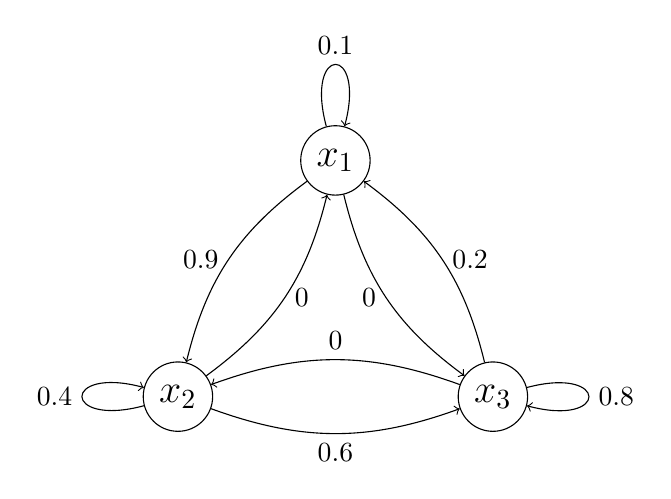
\begin{tikzpicture}[->,main node/.style={circle,draw,font=\sffamily\Large\bfseries}]
    
        \node[main node] at (0,  3) (1) {$x_1$};
        \node[main node] at (-2, 0) (2) {$x_2$};
        \node[main node] at (2,  0) (3) {$x_3$};

        \path[->, every node/.style={font=\sffamily}]
        (1) edge[loop above, looseness=12]  node [above] {$0.1$} (1)
        (1) edge[bend right=20] node [above=.1, left=.1] {$0.9$} (2)
        (1) edge[bend right=20] node [below=.1, left=.1] {$0$} (3)
        
        (2) edge[bend right=20] node [below=.1, right=.1] {$0$} (1)
        (2) edge[loop left, looseness=12] node [left] {$0.4$} (2)
        (2) edge[bend right=20] node [below] {$0.6$} (3)
        
        (3) edge[bend right=20] node [above=.1, right=.1] {$0.2$} (1)
        (3) edge[bend right=20] node [above] {$0$} (2)
        (3) edge[loop right, looseness=12] node [right] {$0.8$} (3);
       
    \end{tikzpicture}    
    \caption{Schema of an example MC.}
    \label{fig:MC_schema}
\end{figure}


We can take a look at a sample from this process (we attach a color to each value for further use):
\begin{equation} \label{eq:example_mc}
    \textcolor{teal}{2}, \textcolor{purple}{3}, \textcolor{purple}{3}, \textcolor{blue}{1}, \textcolor{teal}{2}, \textcolor{purple}{3}, \textcolor{blue}{1}, \textcolor{teal}{2}, \textcolor{purple}{3}, \textcolor{purple}{3}, \textcolor{purple}{3}, \textcolor{purple}{3}, \textcolor{purple}{3}, \textcolor{blue}{1}, \textcolor{teal}{2}, \textcolor{teal}{2}, \textcolor{teal}{2}\text{.}
\end{equation}
\linebreak
We will refer to this example in the next sections.

\section{Hidden Markov Model}  \label{sec:HMM}

A Hidden Markov Model can be seen as a model, where an unobservable (hidden) Markov process influences what we can observe (emission). 


\begin{definition}{Hidden Markov Model} \label{def:hmm}
    
    The Hidden Markov Model is a tuple $\Theta =  (\pi, \textbf{A}, \mathbbm B)$ such that $\pi$, $\textbf{A}$ are the starting probability and the transition matrix of a Markov Chain $X_t$ and $\mathbbm B$ is a family of $N$  parametrized distributions over $\mathcal Y$ such that the emission (observable) process $\{Y_t\}_{t \in \mathbb N}$ has the probability density/mass function $\mathbbm B_i(y) =_d \mathbbm P (Y_t = y | X_t = i)$ and follows the independence assumption:

    \begin{equation*}
        % \mathbb P (Y_{t+1} = y_{t+1} | Y_{1:t} = y_{1:t}, X_{1:t+1} = x_{1:t+1}) = \mathbb P (Y_{t+1} = y_{t+1} | X_{t+1} = x_{t+1}) 
        \mathbb P (Y_{t+1} | Y_{1:t}, X_{1:t+1} ) = \mathbb P (Y_{t+1} | X_{t+1})\text{.}
    \end{equation*}
\end{definition}





\begin{figure}[!ht]
    \centering
    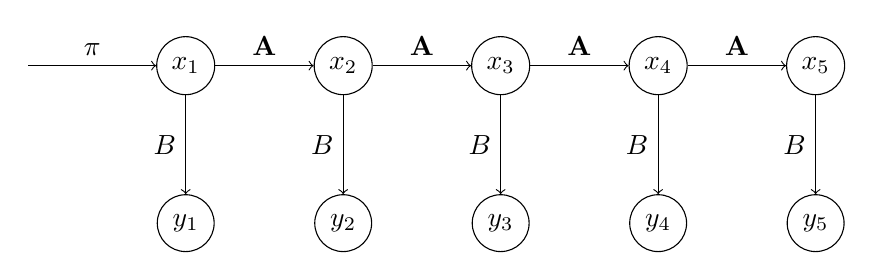
\begin{tikzpicture}[main/.style = {draw, circle}, node distance = 20mm and 10mm] 
        \node[main] (1) {$x_1$};
        \node[main] (2) [right of=1] {$x_2$};
        \node[main] (3) [right of=2] {$x_3$};
        \node[main] (4) [right of=3] {$x_4$};
        \node[main] (5) [right of=4] {$x_5$};


        \node[main] (11) [below of=1] {$y_1$};
        \node[main] (12) [below of=2] {$y_2$};
        \node[main] (13) [below of=3] {$y_3$};
        \node[main] (14) [below of=4] {$y_4$};
        \node[main] (15) [below of=5] {$y_5$};

        \draw[->] (-2, 0) -- node[above] {$\pi$} (1);
        \draw[->] (1) -- node[above] {$\textbf{A}$} (2);
        \draw[->] (2) --  node[above] {$\textbf{A}$} (3);
        \draw[->] (3) -- node[above] {$\textbf{A}$} (4);
        \draw[->] (4) -- node[above] {$\textbf{A}$} (5);
        
        \draw[->] (1) -- node[left] {$\mathbbm B$} (11);
        \draw[->] (2) -- node[left] {$\mathbbm B$} (12);
        \draw[->] (3) -- node[left] {$\mathbbm B$} (13);
        \draw[->] (4) -- node[left] {$\mathbbm B$} (14);
        \draw[->] (5) -- node[left] {$\mathbbm B$} (15);
        
    \end{tikzpicture}    
    \caption{Schema of Hidden Markov Model (for $t \in \mathbb N _{\leq 5}$).}
    \label{fig:model_schema}
\end{figure}

We will denote the length of the observed sequence as $T$. The HMM schema (for $T=5$) is presented in Figure \ref{fig:model_schema}.

% For notational simplicity, let us denote the conditional emission probability as follows: 
% \begin{equation}
%     \mathbbm B_i(y_{t+1}|x_{t+1}) := \mathbb P (Y_{t+1} = y_{t+1} | X_{t+1} = x_{t+1})
% \end{equation}

% The distribution of $Y_t | X_t$ must come from a known and parametrized distribution (for example, discrete, Gaussian, Mixture of Gaussians, Exponential, \ldots ). We will consider a family of distributions $\mathbbm B=\{B_i\}_{i=1}^N$, where the distribution $\mathbbm B_i$ denotes the observed random variable when the state is $i$: 

% \begin{equation}
%     Y_t | X_t = i \quad \sim \quad B_i
% \end{equation}

\pagebreak

\subsection{Example: Discrete HMM} \label{sec:hmm_discrete}

Discrete HMM is the most basic version of the model. We observe a discrete process over $M$ possible values. For simplicity, we can assume that $\mathcal Y \equiv  \{1, 2, \ldots, M\}$.  We can denote the family of distributions $\mathbbm B$ as a stochastic matrix, where $\mathbbm B_{iv} = \mathbbm P(Y_t =  v | X_t = i)$. The probability distribution family $\mathbbm B$ of the emission process has $N \cdot (M - 1)$ parameters.

We will consider an example with hidden states process as in Example \ref{sec:example_mc} and the emission from $\mathcal Y = \{a, b, c, d \}$ with probability:

\begin{equation} \label{eq:ex_B}
    \mathbbm B = \left [\begin{array}{cccc}
        0.50 &  0.15 &  0.15 &  0.20\\
        0.20 &  0.60 &  0.10 &  0.10\\
        0.10 &  0.20 &  0.20 &  0.50\\
    \end{array}\right]\text{.}
\end{equation}

To model the distribution, we need to estimate $3 \cdot (4 - 1) = 9$ parameters.

We observe the following sequence (colors represent the hidden states as in Example \ref{eq:example_mc}):

\begin{equation} \label{eq:ex_gaussian}
    \textcolor{teal}{a}, \textcolor{purple}{c}, \textcolor{purple}{a}, \textcolor{blue}{b}, \textcolor{teal}{b}, \textcolor{purple}{c}, \textcolor{blue}{a}, \textcolor{teal}{a}, \textcolor{purple}{b}, \textcolor{purple}{c}, \textcolor{purple}{b}, \textcolor{purple}{c}, \textcolor{purple}{d}, \textcolor{blue}{c}, \textcolor{teal}{b}, \textcolor{teal}{b}\text{.}
\end{equation}

\subsection{Example: Gaussian HMM} \label{sec:hmm_gaussian}

One of the most popular continuous Hidden Markov Models is Gaussian Hidden Markov Model, which assumes that  $Y_t | X_t = i$ is a multivariate normal distribution: \linebreak $\mathbbm B_i =_d \mathcal N_D (\mu_i, \Sigma_i)$.  The probability distribution family $\mathbbm B$ of the emission process has $N \cdot \big(D + \frac{D(D + 1)}{2}\big)$  parameters. 

Let us consider an HMM with the hidden state from  Example \ref{sec:example_mc} and two-dimensional emission ($\mathcal Y = \mathbbm R^2$) with emission distribution:

\begin{subequations}
    \begin{equation}
        \mathbbm B = \big(\mathcal N_2 (\mu_i, \Sigma_i) \big)_{i=1}^3 \text{,}
    \end{equation}
    \text{ \linebreak where  \linebreak }
    \begin{equation}
        \mu_1 = \left( \begin{array}{c} 0 \\ 0 \\ \end{array} \right),
        \mu_2 = \left( \begin{array}{c} 3 \\ -3 \\ \end{array} \right),
        \mu_3 = \left( \begin{array}{c} 4 \\ 3 \\ \end{array} \right)\text{,}
    \end{equation}
    \begin{equation}
        \Sigma_1 = \left[ \begin{array}{rr}   1.0 & -0.4\\  -0.4 &  0.8 \\ \end{array} \right],
        \Sigma_2 = \left[ \begin{array}{rr}    0.6 & -0.5\\ -0.5 &  1.2 \\ \end{array} \right],
        \Sigma_3 = \left[ \begin{array}{rr}  0.9 &  0.6\\ 0.6 &  1.7 \\ \end{array} \right]\text{.}
    \end{equation} 
\end{subequations}
\linebreak
To model the distribution, we need to estimate $3 \cdot (2 + \frac {2(2+1)} {2}) = 15$ parameters.


% When each hidden state emits observations from a Gaussian distribution, and the starting probability of the hidden states MC is the stationary distribution, the emitted sequence comes from a Mixture of Gaussian with probability $\pi$ and parameters as the HMM, please see Figure \ref{fig:example_gaussian}.



We observe the following sequence (colors represent the hidden states as previously):

\begin{equation*}
    \small
    \begin{aligned}
        &\textcolor{teal}{\left(\begin{array}{c} 2.918\\-2.229\end{array}\right)},
        \textcolor{purple}{\left(\begin{array}{c} 5.320\\4.050\end{array}\right)},
        \textcolor{purple}{\left(\begin{array}{c} 4.626\\0.699\end{array}\right)},
        \textcolor{blue}{\left(\begin{array}{c} 0.709\\-0.372\end{array}\right)},
        \textcolor{teal}{\left(\begin{array}{c} 3.236\\-2.969\end{array}\right)},
        \textcolor{purple}{\left(\begin{array}{c} 2.551\\2.298\end{array}\right)}, \\
        &\textcolor{blue}{\left(\begin{array}{c} 0.318\\-0.740\end{array}\right)},
        \textcolor{teal}{\left(\begin{array}{c} 2.809\\-2.188\end{array}\right)},
        \textcolor{purple}{\left(\begin{array}{c} 4.760\\4.022\end{array}\right)},
        \textcolor{purple}{\left(\begin{array}{c} 3.696\\3.551\end{array}\right)},
        \textcolor{purple}{\left(\begin{array}{c} 5.070\\4.445\end{array}\right)},
        \textcolor{purple}{\left(\begin{array}{c} 3.095\\1.733\end{array}\right)}, \\
        &\textcolor{purple}{\left(\begin{array}{c} 3.491\\3.272\end{array}\right)},
        \textcolor{blue}{\left(\begin{array}{c} -0.725\\-1.437\end{array}\right)},
        \textcolor{teal}{\left(\begin{array}{c} 2.881\\-2.783\end{array}\right)},
        \textcolor{teal}{\left(\begin{array}{c} 4.064\\-3.374\end{array}\right)}\text{.}
    \end{aligned}
\end{equation*}
\linebreak
It can be also plotted as in Figure \ref{fig:example_gaussian}.
\begin{figure}[!ht]
    \centering
    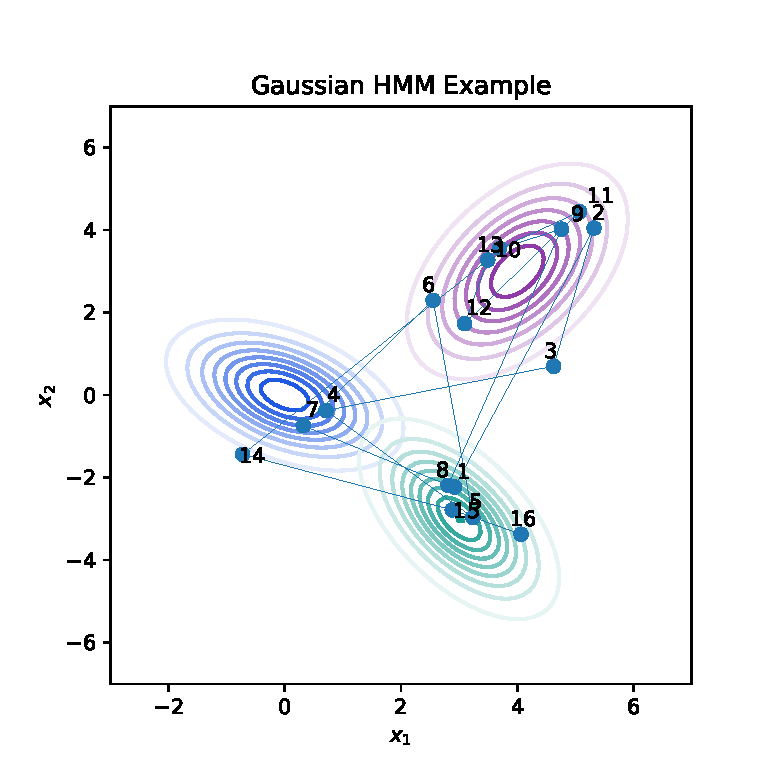
\includegraphics[scale=.7]{gaussian_hmm_example.eps}
    \caption{Gaussian HMM example.}
    \label{fig:example_gaussian}
\end{figure}

Of course, there are several variants of the model with some assumptions on the covariance matrices (in particular diagonal or full but common for all hidden states), which have a smaller number of parameters to be estimated. 

% \subsection{Example 3: Gaussian Mixture Model HMM}

\section{Training and Inference}  \label{sec:hmm_algs}

Let us start with the definition of the likelihood function, which is the base object for this section. 

\begin{definition}{Likelihood}

Let $\Omega$ be a specified set of parameters, $\Tilde{\Theta} \in \Omega$ be a parameter of a distribution and $y_{1:T}$ a realization of a a random vector $Y_{1:T}$ with density or mass function $f(y; \Tilde{\Theta})$. The likelihood function is defined as:

\begin{equation*}
    \mathcal{L}(\Tilde{\Theta}) = \mathcal{L}(\Tilde{\Theta}; y_{1:T}) = \prod_{t=1}^T f(y_t; \Tilde{\Theta})\text{.}
\end{equation*}

\end{definition}

In case of HMM, we fix $N$ and the family of possible distributions $\mathbbm{B}$ and consider $\Omega = \{(\Tilde{\pi}, \Tilde{\textbf{A}}, \Tilde{\mathbbm{B}}): \Tilde{\pi} \in \mathbbm R ^N - \text{stochastic vector}, \Tilde{\textbf{A}} \in \mathbbm R ^{N\times N} - \text{stochastic matrix}, \Tilde{\mathbbm{B}} - \text{family of $n$ parametrized distributions}\}$.
The estimation of models parameters and inference is based on maximization of likelihood.

% \begin{equation*}
%     \mathcal{L}(y_{1:T}) = \prod_{t=1}^T \mathbbm P(Y_t = y_t) = \sum_{x_{1:T} \in \mathcal X ^T} \prod_{t=1}^T \mathbbm P(Y_t = y_t |  X_{1:T} = x_{1:T})  P(X_{1:T} = x_{1:T}) 
% \end{equation*}



The probability of observing a specific sequence is the sum of probabilities of~obtaining a sequence given any possible sequence of hidden states: 
\begin{equation*}
    \mathcal{L}(\Tilde{\Theta}) =  \sum_{x_{1:T} \in \mathcal X ^T} \prod_{t=1}^T \mathbbm B(y_t | x_{1:T}; \Tilde{\Theta}) \mathbbm P(X_{1:T} = x_{1:T}; \Tilde{\Theta}) \text{.}
\end{equation*}
There are $N^T$ possible sequences of hidden states, so calculating each of them separately would be too time-consuming. Before we state the training algorithm, let us specify the algorithm for inferring the most probable sequence of states and two efficient ways of calculating the likelihood of the sequence: the forward and~the~backward algorithms. All of those are based on recurrent formulas and dynamic programming.

\subsection{Viterbi Algorithm}

This algorithm was to inference about the hidden states from a given model $\Tilde{\Theta}$. It allows us to establish which sequence of hidden states is the most probable to emit the~observed sequence. 
%Like the forward algorithm, the Viterbi algorithm is an example of dynamic programming. 

First, let's denote the likelihood of the most probable sequence prefix as:

\begin{equation*}
    \nu_t(j) =  \max_{x_{1:t-1}} \mathbb P (x_{1:t-1}, y_{1:t}, x_t = j)\text{.}
\end{equation*}

We can rewrite the above recursively:

\begin{subequations}
    \begin{equation*}
        \nu_1(j) = \pi_j \mathbbm B_j(y_1)\text{,}
    \end{equation*}
    \begin{equation*}
        \nu_t(j) = \max_{i \in \mathcal X} \nu_{t-1}(i) \textbf{A}_{ij} \mathbbm B_j(y_t)\text{,}
    \end{equation*}
    \begin{equation*}
        \nu = \max_{i \in \mathcal X} \nu_{T}(i)\text{.}
    \end{equation*}
\end{subequations}



We will also consider a matrix of back pointers $\rho$, which stores in the $[t, j]$ element the probability that the state $j$ precedes $x_t$:

\begin{subequations}
    \begin{equation*}
        \rho_{1, j} = \phi\text{,}
    \end{equation*}
    \begin{equation*}
        \rho_{t, j} =  \argmax_{i \in \mathcal X}   \nu_{t-1}(i) \textbf{A}_{ij}  \mathbbm B_j(y_t)\text{,}
    \end{equation*}
    \begin{equation*}
        \rho_ = \argmax_{i \in \mathcal X} \nu_{T}(i)\text{.}
    \end{equation*}
\end{subequations}
The best path ends in $\rho$ and back in time follows the $\rho_{t, j}$ back pointer terms.


\subsection{Forward Algorithm}

The forward probability  for a given model $\Tilde{\Theta}$ is specified as follows:

$$\alpha_{t}(i) = \mathbb P(Y_{1:t} = y_{1:t},  X_t = i)$$
\linebreak
and can be calculated using the recursive formula:

\begin{subequations}
    \begin{equation*}
        \alpha_1(i) = \pi_i \mathbbm B_i (y_1)\text{,}
    \end{equation*}
    \begin{equation*}
        \alpha_t(i) = \sum_{j=1}^n \alpha_{t-1}(j) \textbf{A}_{ji} \mathbbm B_i (y_t)\text{,}
    \end{equation*}
    \begin{equation*}
        \mathbb P(Y_{1:T} = y_{1:T}) = \sum_{i=1}^n \alpha_T(i)\text{.}
    \end{equation*}
\end{subequations}


\subsection{Backward Algorithm}

The backward probability  for a given model $\Tilde{\Theta}$ is specified as follows:

$$\beta_{t}(i) = \mathbb P(Y_{t+1:T} = y_{t+1:T} | X_t = i)$$
\linebreak
and can be calculated using the recursive formula:

\begin{subequations}
    \begin{equation*}
        \beta_T(i) = 1\text{,}
    \end{equation*}
    \begin{equation*}
        \beta_t(i) = \sum_{j=1}^n \textbf{A}_{ij} \mathbbm B_j(y_t) \beta_{t+1}(j)\text{,}
    \end{equation*}
    \begin{equation*}
        \mathbb P(Y_{1:T} = y_{1:T}) = \sum_{j=1}^N \pi_j \mathbbm B_j(y_1) \beta_1(j)\text{.}
    \end{equation*}
\end{subequations}

\subsection{ELBO}

\textbf{E}vidence \textbf{L}ower \textbf{Bo}und (ELBO) is a lower bound on the logarithm of the likelihood function. It uses Jensen's inequality for providing a simpler function to optimize. As~the~likelihood in HMM is quite complicated, in the training, we will maximize ELBO instead of plain likelihood. The below explanation of ELBO is reffered after~\cite{elbo}~and~\cite{elbo_yt}.

First, let us state what we exactly bound: \textit{evidence} is the marginal likelihood of observations $y_{1:T}$. Now, let us recall the definition of Kullback-Leibler divergence, which is a way of measuring similarity between two likelihood functions. 

\begin{definition}{KL Divergence}

Let us have two probability measures $p$ and $q$ defined at the same measurable space $\mathcal X$. %, such that $q$ is an approximation of $p$. %, such that $p$ is absolutly contiunuous with respect to $q$. 
Typically, $p$ represents the true distribution of data and $q$ approximates $p$. 

\begin{equation*}
    KL(q \Vert p) = \int_{\mathcal X}  \Bigg[ \log \frac{q(x)}{p(x)} \Bigg] dq(x)
\end{equation*}

    % Let us consider a posterior distribution $p$ and a estimation of the posterior $q$. Kullback-Leibler divergence between $q$ and $p$ is the following expected value with respect to the probability measure $q$:

    % \begin{equation}
    %     KL(q \Vert p) = \mathbbm E_q \Bigg[ \log \frac{q(x)}{p(y | x)} \Bigg]
    % \end{equation}

    Please note, that KL divergence is not a distance metric, as it is not symmetric and the triangle inequality does not hold.
\end{definition}

We can provide also a simpler formula for KL divergence for discrete case:

\begin{equation} \label{eq:kl_d}
    KL(q \Vert p) = \sum_{x \in \mathcal X} q(x) \Bigg[ \log \frac{q(x)}{p(x)} \Bigg] \text{,}
\end{equation}
or  for continuous emission over  $\mathbbm R^n$:
 \begin{equation*}
     KL(p \Vert q) = \int_{\mathbbm R^n} q(x) \Bigg[ \log \frac{q(x)}{p(x)} \Bigg] dx\text{,}
 \end{equation*}
or more generally using the expected value (with respect to $X \sim q(x)$):
\begin{equation*}
    KL(p \Vert q) = \mathbbm E_{q(x)} \Bigg[ \log \frac{q(x)}{p(x)} \Bigg] dx\text{.}
\end{equation*}

Now, let us recall the inequality mentioned.

\begin{theorem} {Jensen's Inequality}

Let $f$ be an concave function. Jensen's inequality for the random variable $X$ is:

\begin{equation*}
    f( \mathbbm E [X] ) \geq  \mathbbm E [f(X)] \text{.}
\end{equation*}
    
\end{theorem}

It is easy to show, that $\log(\cdot)$ is a concave function. We will use this fact when defining ELBO. 

\begin{definition} {ELBO}

    Let us have two dependent random variables $Y$ over the measurable space $\mathcal  Y$ (observations) and $X$ over the measurable space $\mathcal  X$ (hidden layer), the marginal probability of observations $q(y)$, joined probability $q(y, x)$ and conditional pobability $q(y|x)$ and the probability of the hidden layer $p(x)$. Typically, $p$ represents the true distribution of the hidden states and $q$ represent the approximate distribution of observations. We apply the Jensen's inequality to the logarithm of the probability to get the formula for \textbf{E}vidence \textbf{L}ower \textbf{Bo}und (ELBO) (for  a continuous case):

    \begin{equation} \label{eq:elbo}
    \begin{aligned}
        \log p(y) & =  \log \int_{\mathcal X} p(y, x) dx =  \log \int_{\mathcal X} p(y, x) \frac{q(x)}{q(x)} dx =  \log \int_{\mathcal X} q(x) \frac{p(y, x)}{q(x)} dx \geq \\ & \geq  \int_{\mathcal X} q(x) \big[\log p(y, x) -  \log q(x)\big] dx %= \int_{\mathcal X} p(x) \big[\log q(y | x) + \log q(x) -  \log p(x)\big] dx \text{.}
    \end{aligned}
    \end{equation}

In case of discrete $\mathcal X$, we consider a sum instead of a integral. We can also state the Inequality (\ref{eq:elbo})  using the expected value (with respect to $X \sim q(x)$):

\begin{equation*}
    \log p(y) \geq \mathbbm{E}_{q(x)} \Bigg[\log\Big(\frac{p(y, x)}{q(x)}\Big)\Bigg]
\end{equation*}
\end{definition}

% Let us also show the relationship between KL divergence and ELBO:

% \begin{equation}
% \begin{aligned}
%        & ELBO(p) = \mathbbm E_q \log p(y, x) -  \mathbbm E_q \log q(x) =  
%      \\
%      & = \mathbbm E_q \log p(y | x) + \mathbbm E_q \log  p(x)  -  \mathbbm E_q \log q(x) = 
%      - KL (q \Vert p) + \mathbbm E_q \log  p(x) 
% \end{aligned}
% \end{equation}

ELBO and KL divergence are closely related. They are also often used in variational inference when we cannot calculate the posterior distribution $p(x | y)$ and want to approximate it by a tractable distribution $q(x)$.
To get a distribution close to the posterior, we play with the parameters of the tractable distribution as to minimize the KL divergence: $KL\big(q(x) \Vert p(x | y)\big)$. Let us use the elaborate the Equation (\ref{eq:kl_d}) (similarly calculations can be done for the continuous case):

\begin{equation*}
\begin{aligned}
    KL\big(q(x) \Vert p(x | y)\big) & = \mathbbm{E}_{q(x)} \Bigg[ \log \frac{q(x)}{p(x|y)} \Bigg] = \\
    & = - \mathbbm{E}_{q(x)} \Bigg[ \log \frac{p(x|y)}{q(x)} \Bigg] \text{,}
\end{aligned}
\end{equation*}
using the the Bayesian rule:
\begin{equation*}
    KL\big(q(x) \Vert p(x | y)\big) = - \mathbbm{E}_{q(x)} \Bigg[ \log \frac{p(x, y)}{p(y) q(x)} \Bigg] \text{,}
\end{equation*} 
using the properties of logarithm:
\begin{equation*}
    KL\big(q(x) \Vert p(x | y)\big) = - \mathbbm{E}_{q(x)} \Bigg[ \log \frac{p(x, y)}{q(x)} \Bigg] +  \mathbbm{E}_{q(x)} \Big[ \log p(y) \Big] \text{,} \\
\end{equation*}
as $\log p(y)$ does not depend on $x$:
\begin{equation*}
\begin{aligned}
    KL\big(q(x) \Vert p(x | y)\big) & = - \mathbbm{E}_{q(x)} \Bigg[ \log \frac{p(x, y)}{q(x)} \Bigg] +  \log p(y)  \text{.}
\end{aligned}
\end{equation*}
\linebreak
So we can state that:

\begin{equation*}
    \log p(y) = KL\big(q(x) \Vert p(x | y)\big) + \mathbbm{E}_{q(x)}  \big[\log p(y, x) -  \log q(x)\big]\text{.}
\end{equation*}

As $p(y)$ is a constant value, we see that minimizing KL divergence between the posterior and its approximation is equivalent to maximizng ELBO (see Equation (\ref{eq:elbo})). 

\subsection{ELBO for HMM}

Let us recall the formula for the likelihood of the sequence: \linebreak
% \begin{equation*}
    $\mathcal{L}(\Tilde{\Theta}; y_{1:T}) = \mathbbm P(Y_{1:T}=y_{1:T} | \Tilde{\Theta}) =: \mathbbm P_{\Tilde{\Theta}}(Y_{1:T}=y_{1:T})$,
% \end{equation*}
and the log-likelihood:  \linebreak
% \begin{equation*}
    $\ell (\Tilde{\Theta}; y_{1:T}) := \log \mathcal{L}(\Tilde{\Theta}; y_{1:T}) = \log \mathbbm P_{\Tilde{\Theta}}(Y_{1:T}=y_{1:T})\text{.}$
% \end{equation*}

% We will denote the approximate probability as in the next section, where the index of the iteration is denoted as $k$ and the current model estimate as $\Theta^{(k)}$.
Let us calculate the ELBO for HMM (where the true distribution comes from the model $\Theta$ and the approximate one comes from the model $\Tilde{\Theta}$):

\begin{equation*}
    \begin{aligned}
        \ell (\Tilde{\Theta}; y_{1:T}) = &\log \mathbbm P_{\Tilde{\Theta}}(Y_{1:T}=y_{1:T}) = \log \Bigg( \sum_{x_{1:T} \in \mathcal X^T} \mathbbm P_{\Tilde{\Theta}}(Y_{1:T}=y_{1:T}, X_{1:T}=x_{1:T}) \Bigg) = \\
        & = \log \Bigg( \sum_{x_{1:T} \in \mathcal X^T} \mathbbm P_{\Tilde{\Theta}}(Y_{1:T}=y_{1:T}, X_{1:T}=x_{1:T}) \frac{\mathbbm P_{\Theta}(X_{1:T}=x_{1:T})}{\mathbbm P_{\Theta}(X_{1:T}=x_{1:T})} \Bigg) \geq \\
        & \geq \sum_{x_{1:T} \in \mathcal X^T} \mathbbm P_{\Theta}(X_{1:T}=x_{1:T}) \log \Bigg(  \frac{\mathbbm P_{\Tilde{\Theta}}(Y_{1:T}=y_{1:T}, X_{1:T}=x_{1:T})}{\mathbbm P_{\Theta}(X_{1:T}=x_{1:T})} \Bigg) =: \ell^* \text{.}\\
    \end{aligned}
\end{equation*}
\linebreak
Now we can transform the approximate probability to express it using HMM parameter estimators:
\begin{equation*}
    \begin{aligned}
        & \ell^* (\Tilde{\Theta}; y_{1:T}) = \\ & \sum_{x_{1:T} \in \mathcal X^T} \mathbbm P_{\Theta}(X_{1:T}=x_{1:T}) \log \Bigg( \frac{\mathbbm P_{\Tilde{\Theta}}(X_{1:T}=x_{1:T}) \cdot  \mathbbm P_{\Tilde{\Theta}}(Y_{1:T}=y_{1:T} | X_{1:T}=x_{1:T})}{\mathbbm P_{\Theta}(X_{1:T}=x_{1:T})} \Bigg) = \\
        % & = \sum_{x_{1:T} \in \mathcal X^T} \mathbbm P_{\Theta}(X_{1:T}=x_{1:T}) \log \Bigg(  \frac{\mathbbm P_{\Tilde{\Theta}}(X_{1:T}=x_{1:T}) \cdot \prod_{t=1}^T \mathbbm P_{\Tilde{\Theta}}(Y_{t}=y_{t} | X_{1:T}=x_{1:T})}{\mathbbm P_{\Theta}(X_{1:T}=x_{1:T})} \Bigg) = \\
        & = \sum_{x_{1:T} \in \mathcal X^T} \mathbbm P_{\Theta}(X_{1:T}=x_{1:T}) \log \Bigg( \\ & \quad \quad \quad \frac{\mathbbm P_{\Tilde{\Theta}}(X_{1}=x_{1}) \cdot \prod_{t=1}^{T-1} \mathbbm P_{\Tilde{\Theta}}(X_{t+1}=x_{t+1}|X_{t}=x_{t})  \cdot \prod_{t=1}^T \mathbbm P_{\Tilde{\Theta}}(Y_{t}=y_{t} | X_{1:T}=x_{1:T})}{\mathbbm P_{\Theta}(X_{1:T}=x_{1:T})} \Bigg) = \\
        % & = \sum_{x_{1:T} \in \mathcal X^T} \mathbbm P_{\Theta}(X_{1:T}=x_{1:T}) \log \Bigg( \\ & \frac{\mathbbm P_{\Tilde{\Theta}}(X_{1}=x_{1}) \cdot \prod_{t=1}^{T-1} \mathbbm P_{\Tilde{\Theta}}(X_{t+1}=x_{t+1}|X_{t}=x_{t})  \cdot \prod_{t=1}^T \mathbbm P_{\Tilde{\Theta}}(Y_{t}=y_{t} | X_{t}=x_{t})}{\mathbbm P_{\Theta}(X_{1:T}=x_{1:T})} \Bigg) = \\
        & = \sum_{x_{1:T} \in \mathcal X^T} \mathbbm P_{\Theta}(X_{1:T}=x_{1:T}) \log \Bigg( \frac{\Tilde{\pi}_{x_1} \cdot \prod_{t=1}^{T-1} \Tilde{\textbf{A}}_{x_t, x_{t+1}}  \cdot \prod_{t=1}^T \Tilde{\mathbbm B}_{x_t}(y_t)}{\mathbbm P_{\Theta}(X_{1:T}=x_{1:T})} \Bigg) \text{,}
    \end{aligned}
\end{equation*}
\linebreak
and express ELBO in summands:
\begin{equation*}
    \begin{aligned}
         \ell^* (\Tilde{\Theta}; y_{1:T}) = & \sum_{x_{1:T} \in \mathcal X^T} \mathbbm P_{\Theta}(X_{1:T}=x_{1:T}) \log  \Tilde{\pi}_{x_1}  +\\ & +  \sum_{x_{1:T} \in \mathcal X^T} \mathbbm P_{\Theta}(X_{1:T}=x_{1:T}) \sum_{t=1}^{T-1}  \log \Tilde{\textbf{A}}_{x_t, x_{t+1}}  +\\ & +  \sum_{x_{1:T} \in \mathcal X^T} \mathbbm P_{\Theta}(X_{1:T}=x_{1:T}) \sum_{t=1}^T \log   \Tilde{\mathbbm B}_{x_t}(y_t)  +\\ & -  \sum_{x_{1:T} \in \mathcal X^T} \mathbbm P_{\Theta}(X_{1:T}=x_{1:T}) \log \Big(\mathbbm P_{\Theta}(X_{1:T}=x_{1:T}) \Big)\text{,}
    \end{aligned}
\end{equation*}
and reduce the sums:
\begin{equation*}
    \begin{aligned}
        \ell^* (\Tilde{\Theta}; y_{1:T}) = & \sum_{i=1}^N \mathbbm P_{\Theta}(X_{1}=i) \log  \Tilde{\pi}_{i}  +\\ 
        & +  \sum_{t=1}^{T-1} \sum_{i=1}^N  \sum_{j=1}^N \mathbbm P_{\Theta}(X_{t}=i, X_{t+1}=j) \log  \Tilde{\textbf{A}}_{ij}  +\\ 
        & +  \sum_{t=1}^T \sum_{i=1}^N \mathbbm P_{\Theta}(X_{t}=i) \log   \Tilde{\mathbbm B}_{i}^{(k)}(y_t)  +\\ 
        & -  \sum_{x_{1:T} \in \mathcal X^T} \mathbbm P_{\Theta}(X_{1:T}=x_{1:T}) \log \Big(\mathbbm P_{\Theta}(X_{1:T}=x_{1:T}) \Big)\text{.}
    \end{aligned}
\end{equation*}

% \pagebreak

% Let us recall the formula for the likelihood of the sequence:
% \begin{equation*}
%     \mathcal{L}(\Tilde{\Theta}; y_{1:T}) = \mathbbm P(Y_{1:T}=y_{1:T}) = \prod_{t=1}^T \mathbbm P(Y_{t}=y_t) = \mathbbm P(Y_{1} = y_1) \prod_{t=2}^T \mathbbm P(Y_{t}=y_t)
% \end{equation*}

% and the log-likelihood:
% \begin{equation*}
%     \ell (y_{1:T}) = \log \mathbbm P(Y_{1:T}=y_{1:T}) = \sum_{t=1}^T \log \mathbbm P(Y_{t}=y_t) = \log \mathbbm P(Y_{1} = y_1) + \sum_{t=2}^T \log \mathbbm P(Y_{t}=y_t)
% \end{equation*}

% Now, we will derive the ELBO as in the difinition. Using the law of total probability:
% \begin{equation*}
% \begin{aligned}
%     & = \log \Bigg[ \sum_{i=1}^N \sum_{j=1}^N \mathbbm P(Y_{1} = y_1, X_1 = i, X_2 = j) \Bigg] +  \\
%     & + \sum_{t=2}^{T-1} \log  \Big[ \sum_{i=1}^N \sum_{j=1}^N \mathbbm P(Y_{t} = y_t,  X_t = i, X_{t+1} = j) \Big] +  \\
%     & + \log  \Big[ \sum_{i=1}^N \mathbbm P(Y_{T} = y_T,  X_T = i) \Big]
% \end{aligned}
% \end{equation*}

% Adding a component for probability estimator:
% \begin{equation*}
% \begin{aligned}
%     & = \log  \Bigg[ \sum_{i=1}^N  \sum_{j=1}^N \mathbbm P(Y_{1} = y_1, X_1 = i, X_2 = j) \frac{\mathbbm P (X_1 = i, X_2 = j | \Theta ^{(k)})}{\mathbbm P (X_1 = i, X_2 = j | \Theta ^{(k)})} \Bigg] +  \\
%     & + \sum_{t=2}^{T-1} \log  \Big[ \sum_{i=1}^N \sum_{j=1}^N \mathbbm P(Y_{t} = y_t,  X_t = i, X_{t+1} = j) \frac{\mathbbm P (X_t = i, X_{t+1} = j | \Theta ^{(k)})}{\mathbbm P (X_t = i, X_{t+1} = j | \Theta ^{(k)})} \Big] + \\
%     & + \log  \Big[ \sum_{i=1}^N \mathbbm P(Y_{T} = y_T,  X_T = i) \frac{\mathbbm P (X_T = i| \Theta ^{(k)})}{\mathbbm P (X_T = i | \Theta ^{(k)})} \Big]
% \end{aligned}
% \end{equation*}

% And using Jensen's inequality to get ELBO:
% \begin{equation*}
% \begin{aligned}
%     & ELBO =  \sum_{i=1}^N  \sum_{j=1}^N \mathbbm P (X_1 = i, X_2 = j | \Theta ^{(k)}) \log  \Bigg[\frac{ \mathbbm P(Y_{1} = y_1, X_1 = i, X_2 = j) }{\mathbbm P (X_1 = i, X_2 = j | \Theta ^{(k)})} \Bigg] +  \\
%     & + \sum_{t=2}^{T-1} \sum_{i=1}^N \sum_{j=1}^N \mathbbm P (X_t = i, X_{t+1} = j | \Theta ^{(k)}) \log  \Big[  \frac{ \mathbbm P(Y_{t} = y_t,  X_t = i, X_{t+1} = j)}{\mathbbm P (X_t = i, X_{t+1} = j | \Theta ^{(k)})} \Big] + \\
%     & + \sum_{i=1}^N \mathbbm P (X_T = i| \Theta ^{(k)}) \log  \Big[ \frac{ \mathbbm P(Y_{T} = y_T,  X_T = i) }{\mathbbm P (X_T = i | \Theta ^{(k)})} \Big] 
% \end{aligned}
% \end{equation*}

% Now we need to transform the formula to get the parameters of the HMM in it:
% % \begin{equation*}
% % \begin{aligned}
% %     & =  \sum_{i=1}^N  \sum_{j=1}^N \mathbbm P (X_1 = i, X_2 = j | \Theta ^{(k)}) \log  \Bigg[\frac{ 
% %     \mathbbm P(Y_{1} = y_1 |  X_1 = i, X_2 = j) \mathbbm P(X_2 = j | X_1 = i) \mathbbm P(X_1 = i) 
% %     }{\mathbbm P (X_1 = i, X_2 = j | \Theta ^{(k)})} \Bigg] +  \\
% %     & + \sum_{t=2}^{T-1} \sum_{i=1}^N \sum_{j=1}^N \mathbbm P (X_t = i, X_{t+1} = j | \Theta ^{(k)}) \log  \Big[  \frac{ 
% %     \mathbbm P(Y_{t} = y_t |  X_t = i, X_{t+1} = j) \mathbbm P(X_{t+1} = j | X_t = i) \mathbbm P (X_t = i)
% %     }{\mathbbm P (X_t = i, X_{t+1} = j | \Theta ^{(k)})} \Big] + \\
% %     & + \sum_{i=1}^N \mathbbm P (X_T = i| \Theta ^{(k)}) \log  \Big[ \frac{ 
% %     \mathbbm P(Y_{T} = y_T |  X_T = i) \mathbbm P(X_T = i) 
% %     }{\mathbbm P (X_T = i | \Theta ^{(k)})} \Big] = 
% % \end{aligned}
% % \end{equation*}
% \begin{equation*}
% \begin{aligned}
%     & =  \sum_{i=1}^N  \sum_{j=1}^N \mathbbm P (X_1 = i, X_2 = j | \Theta ^{(k)}) \log  \Bigg[\frac{ 
%     \mathbbm P(Y_{1} = y_1 |  X_1 = i) \mathbbm P(X_2 = j | X_1 = i) \mathbbm P(X_1 = i) 
%     }{\mathbbm P (X_1 = i, X_2 = j | \Theta ^{(k)})} \Bigg] +  \\
%     & + \sum_{t=2}^{T-1} \sum_{i=1}^N \sum_{j=1}^N \mathbbm P (X_t = i, X_{t+1} = j | \Theta ^{(k)}) \log  \Big[  \frac{ 
%     \mathbbm P(Y_{t} = y_t |  X_t = i) \mathbbm P(X_{t+1} = j | X_t = i) \mathbbm P (X_t = i)
%     }{\mathbbm P (X_t = i, X_{t+1} = j | \Theta ^{(k)})} \Big] + \\
%     & + \sum_{i=1}^N \mathbbm P (X_T = i| \Theta ^{(k)}) \log  \Big[ \frac{ 
%     \mathbbm P(Y_{T} = y_T |  X_T = i) \mathbbm P(X_T = i) 
%     }{\mathbbm P (X_T = i | \Theta ^{(k)})} \Big] = 
% \end{aligned}
% \end{equation*}

% \begin{equation*}
% \begin{aligned}
%     & =  \sum_{i=1}^N  \sum_{j=1}^N \mathbbm P (X_1 = i, X_2 = j | \Theta ^{(k)}) \log  \Bigg[\frac{ 
%     \mathbbm B_i(y_1) \textbf{A}_{ij} \mathbbm P(X_1 = i) 
%     }{\mathbbm P (X_1 = i, X_2 = j | \Theta ^{(k)})} \Bigg] +  \\
%     & + \sum_{t=2}^{T-1} \sum_{i=1}^N \sum_{j=1}^N \mathbbm P (X_t = i, X_{t+1} = j | \Theta ^{(k)}) \log  \Big[  \frac{ 
%     \mathbbm B_i(y_t) \textbf{A}_{ij} \mathbbm P (X_t = i)
%     }{\mathbbm P (X_t = i, X_{t+1} = j | \Theta ^{(k)})} \Big] + \\
%     & + \sum_{i=1}^N \mathbbm P (X_T = i| \Theta ^{(k)}) \log  \Big[ \frac{ 
%     \mathbbm B_i(y_T) \mathbbm P(X_T = i) 
%     }{\mathbbm P (X_T = i | \Theta ^{(k)})} \Big] =
% \end{aligned}
% \end{equation*}

% Now we will use the properties of the logarithm:
% \begin{equation*}
% \begin{aligned}
%     & =  \sum_{i=1}^N  \sum_{j=1}^N \mathbbm P (X_1 = i, X_2 = j | \Theta ^{(k)}) \log  \mathbbm B_i(y_1) + \\
%     & + \sum_{i=1}^N  \sum_{j=1}^N \mathbbm P (X_1 = i, X_2 = j | \Theta ^{(k)}) \log   \textbf{A}_{ij} + \\
%     & +  \sum_{i=1}^N  \sum_{j=1}^N \mathbbm P (X_1 = i, X_2 = j | \Theta ^{(k)}) \log   \mathbbm P(X_1 = i) +  \\
%     & - \sum_{i=1}^N  \sum_{j=1}^N \mathbbm P (X_1 = i, X_2 = j | \Theta ^{(k)}) \log  \mathbbm P (X_1 = i, X_2 = j | \Theta ^{(k)}) +  \\ % first summend
%     & + \sum_{t=2}^{T-1} \sum_{i=1}^N \sum_{j=1}^N \mathbbm P (X_t = i, X_{t+1} = j | \Theta ^{(k)}) \log      \mathbbm B_i(y_t) + \\
%      & + \sum_{t=2}^{T-1} \sum_{i=1}^N \sum_{j=1}^N \mathbbm P (X_t = i, X_{t+1} = j | \Theta ^{(k)}) \log   \textbf{A}_{ij} + \\
%      & + \sum_{t=2}^{T-1} \sum_{i=1}^N \sum_{j=1}^N \mathbbm P (X_t = i, X_{t+1} = j | \Theta ^{(k)}) \log      \mathbbm P (X_t = i) + \\
%      & - \sum_{t=2}^{T-1} \sum_{i=1}^N \sum_{j=1}^N \mathbbm P (X_t = i, X_{t+1} = j | \Theta ^{(k)}) \log  \mathbbm P (X_t = i, X_{t+1} = j | \Theta ^{(k)}) + \\ % second summand
%     & + \sum_{i=1}^N \mathbbm P (X_T = i| \Theta ^{(k)}) \log      \mathbbm B_i(y_T) + \\
%     & + \sum_{i=1}^N \mathbbm P (X_T = i| \Theta ^{(k)}) \log \mathbbm P(X_T = i)  + \\
%     & - \sum_{i=1}^N \mathbbm P (X_T = i| \Theta ^{(k)}) \mathbbm P (X_T = i | \Theta ^{(k)})
% \end{aligned}
% \end{equation*}

% Let us also simplify the formula:
% \begin{equation*}
% \begin{aligned}
%     & =  \sum_{i=1}^N \mathbbm P (X_1 = i| \Theta ^{(k)}) \log  \mathbbm B_i(y_1) + \\
%     & + \sum_{i=1}^N  \sum_{j=1}^N \mathbbm P (X_1 = i, X_2 = j | \Theta ^{(k)}) \log   \textbf{A}_{ij} + \\
%     & +  \sum_{i=1}^N  \mathbbm P (X_1 = i | \Theta ^{(k)}) \log   \mathbbm P(X_1 = i) +  \\
%     & - \sum_{i=1}^N  \sum_{j=1}^N \mathbbm P (X_1 = i, X_2 = j | \Theta ^{(k)}) \log  \mathbbm P (X_1 = i, X_2 = j | \Theta ^{(k)}) +  \\ % first summend
%     & + \sum_{t=2}^{T-1} \sum_{i=1}^N \mathbbm P (X_t = i | \Theta ^{(k)}) \log      \mathbbm B_i(y_t) + \\
%      & + \sum_{t=2}^{T-1} \sum_{i=1}^N \sum_{j=1}^N \mathbbm P (X_t = i, X_{t+1} = j | \Theta ^{(k)}) \log   \textbf{A}_{ij} + \\
%      & + \sum_{t=2}^{T-1} \sum_{i=1}^N  \mathbbm P (X_t = i | \Theta ^{(k)}) \log      \mathbbm P (X_t = i) + \\
%      & - \sum_{t=2}^{T-1} \sum_{i=1}^N \sum_{j=1}^N \mathbbm P (X_t = i, X_{t+1} = j | \Theta ^{(k)}) \log  \mathbbm P (X_t = i, X_{t+1} = j | \Theta ^{(k)}) + \\ % second summand
%     & + \sum_{i=1}^N \mathbbm P (X_T = i| \Theta ^{(k)}) \log      \mathbbm B_i(y_T) + \\
%     & + \sum_{i=1}^N \mathbbm P (X_T = i| \Theta ^{(k)}) \log \mathbbm P(X_T = i)  + \\
%     & - \sum_{i=1}^N \mathbbm P (X_T = i| \Theta ^{(k)}) \log  \mathbbm P (X_T = i | \Theta ^{(k)})
% \end{aligned}
% \end{equation*}

% And reorder the sums:
% \begin{equation*}
% \begin{aligned}
%     & =  \sum_{t=1}^{T} \sum_{i=1}^N \mathbbm P (X_t = i| \Theta ^{(k)}) \log  \mathbbm B_i(y_t) + \\
%     & +  \sum_{i=1}^N  \mathbbm P (X_1 = i | \Theta ^{(k)}) \log \pi_i +  \\
%     & + \sum_{t=1}^{T-1} \sum_{i=1}^N  \sum_{j=1}^N \mathbbm P (X_t = i, X_{t+1} = j | \Theta ^{(k)}) \log   \textbf{A}_{ij} + \\
%     & +  \sum_{t=1}^{T} \sum_{i=1}^N  \mathbbm P (X_t = i | \Theta ^{(k)}) \log   \mathbbm P(X_t = i) +  \\
%     & - \sum_{t=1}^{T-1} \sum_{i=1}^N \sum_{j=1}^N \mathbbm P (X_t = i, X_{t+1} = j | \Theta ^{(k)}) \log  \mathbbm P (X_t = i, X_{t+1} = j | \Theta ^{(k)}) + \\ % second summand
%     & - \sum_{i=1}^N \mathbbm P (X_T = i| \Theta ^{(k)}) \log \mathbbm P (X_T = i | \Theta ^{(k)})
% \end{aligned}
% \end{equation*}

% It is enough to maximize (beacuse the last 3 terms simplify to something positive and we get a lower bound of ELBO?? The better approximation, the lower the gap)
% \begin{equation*}
% \begin{aligned}
%     & \ell^* =  \sum_{t=1}^{T} \sum_{i=1}^N \mathbbm P (X_t = i| \Theta ^{(k)}) \log  \mathbbm B_i(y_t) + \\
%     & +  \sum_{i=1}^N  \mathbbm P (X_1 = i | \Theta ^{(k)}) \log \pi_i +  \\
%     & \quad + \sum_{t=1}^{T-1} \sum_{i=1}^N  \sum_{j=1}^N \mathbbm P (X_t = i, X_t+1 = j | \Theta ^{(k)}) \log   \textbf{A}_{ij} 
%     % & \quad +  \sum_{t=1}^{T} \sum_{i=1}^N  \mathbbm P (X_1 = i | \Theta ^{(k)}) \log   \mathbbm P(X_t = i) 
% \end{aligned}
% \end{equation*}
% %--------

% \pagebreak


% \begin{equation*}
% \begin{aligned}
%     & = \log  \Bigg[ \sum_{i=1}^N  \sum_{j=1}^N \mathbbm P(Y_{1} = y_1, X_1 = i | X_2 = j) \mathbbm P(X_2 = j) \frac{\mathbbm P (X_1 = i, X_2 = j | \Theta ^{(k)})}{\mathbbm P (X_1 = i, X_2 = j | \Theta ^{(k)})} \Bigg] +  \\
%     & + \sum_{t=2}^{T-1} \log  \Big[ \sum_{i=1}^N \sum_{j=1}^N \mathbbm P(Y_{t} = y_t,  X_t = i | X_{t+1} = j) \mathbbm P(X_{t+1} = j) \frac{\mathbbm P (X_t = i, X_{t+1} = j | \Theta ^{(k)})}{\mathbbm P (X_t = i, X_{t+1} = j | \Theta ^{(k)})} \Big] + \\
%     & + \log  \Big[ \sum_{i=1}^N \mathbbm P(Y_{T} = y_T,  X_T = i) \frac{\mathbbm P (X_T = i| \Theta ^{(k)})}{\mathbbm P (X_T = i | \Theta ^{(k)})} \Big]
% \end{aligned}
% \end{equation*}

% \begin{equation*}
% \begin{aligned}
%     & = \log  \Bigg[ \sum_{i=1}^N  \sum_{j=1}^N \mathbbm P(Y_{1} = y_1, X_1 = i) \mathbbm P(X_2 = j) \frac{\mathbbm P (X_1 = i, X_2 = j | \Theta ^{(k)})}{\mathbbm P (X_1 = i, X_2 = j | \Theta ^{(k)})} \Bigg] +  \\
%     & + \sum_{t=2}^{T-1} \log  \Big[ \sum_{i=1}^N \sum_{j=1}^N \mathbbm P(Y_{t} = y_t,  X_t = i) \mathbbm P(X_{t+1} = j) \frac{\mathbbm P (X_t = i, X_{t+1} = j | \Theta ^{(k)})}{\mathbbm P (X_t = i, X_{t+1} = j | \Theta ^{(k)})} \Big] + \\
%     & + \log  \Big[ \sum_{i=1}^N \mathbbm P(Y_{T} = y_T,  X_T = i) \frac{\mathbbm P (X_T = i| \Theta ^{(k)})}{\mathbbm P (X_T = i | \Theta ^{(k)})} \Big]
% \end{aligned}
% \end{equation*}

% And using Jensen's inequality to get ELBO:

% \begin{equation*}
% \begin{aligned}
%     &\ell^* = \log \sum_{i=1}^N  \sum_{j=1}^N \mathbbm P (X_1 = i, X_2 = j | \Theta ^{(k)}) \log \Bigg[ \frac{\mathbbm P(Y_{1} = y_1, X_1 = i) \mathbbm P(X_2 = j) } {\mathbbm P (X_1 = i, X_2 = j | \Theta ^{(k)})} \Bigg] +  \\
%     & + \sum_{t=2}^{T-1} \sum_{i=1}^N \sum_{j=1}^N \mathbbm P (X_t = i, X_{t+1} = j | \Theta ^{(k)})   \log  \Big[ \frac{ \mathbbm P(Y_{t} = y_t,  X_t = i) \mathbbm P(X_{t+1} = j)}{\mathbbm P (X_t = i, X_{t+1} = j | \Theta ^{(k)})} \Big] + \\
%     & + \sum_{i=1}^N \mathbbm P (X_T = i | \Theta ^{(k)}) \log  \Big[ \frac{ \mathbbm P(Y_{T} = y_T,  X_T = i) }{\mathbbm P (X_T = i | \Theta ^{(k)})} \Big] = 
% \end{aligned}
% \end{equation*}


% \begin{equation*}
% \begin{aligned}
%     & = \log \sum_{i=1}^N  \sum_{j=1}^N \mathbbm P (X_1 = i, X_2 = j | \Theta ^{(k)}) \log \Bigg[ \frac{\mathbbm P(Y_{1} = y_1 | X_1 = i) \mathbbm P(X_1 = i) \mathbbm P(X_2 = j) } {\mathbbm P (X_1 = i, X_2 = j | \Theta ^{(k)})} \Bigg] +  \\
%     & + \sum_{t=2}^{T-1} \sum_{i=1}^N \sum_{j=1}^N \mathbbm P (X_t = i, X_{t+1} = j | \Theta ^{(k)})   \log  \Big[ \frac{ \mathbbm P(Y_{t} = y_t |  X_t = i) \mathbbm P( X_t = i)  \mathbbm P(X_{t+1} = j)}{\mathbbm P (X_t = i, X_{t+1} = j | \Theta ^{(k)})} \Big] + \\
%     & + \sum_{i=1}^N \mathbbm P (X_T = i | \Theta ^{(k)}) \log  \Big[ \frac{ \mathbbm P(Y_{T} = y_T|  X_T = i) \mathbbm P(X_T = i) }{\mathbbm P (X_T = i | \Theta ^{(k)})} \Big]
% \end{aligned}
% \end{equation*}


% \begin{equation*}
% \begin{aligned}
%     & = \log \sum_{i=1}^N  \sum_{j=1}^N \mathbbm P (X_1 = i, X_2 = j | \Theta ^{(k)}) \log \Bigg[ \frac{\mathbbm B_i(y_1) \pi_i \textbf{A}_{ij} } {\mathbbm P (X_1 = i, X_2 = j | \Theta ^{(k)})} \Bigg] +  \\
%     & + \sum_{t=2}^{T-1} \sum_{i=1}^N \sum_{j=1}^N \mathbbm P (X_t = i, X_{t+1} = j | \Theta ^{(k)})   \log  \Big[ \frac{ \mathbbm B_i(y_t) \textbf{A}_{ij}}{\mathbbm P (X_t = i, X_{t+1} = j | \Theta ^{(k)})} \Big] + \\
%     & + \sum_{i=1}^N \mathbbm P (X_T = i | \Theta ^{(k)}) \log  \Big[ \frac{ \mathbbm P(Y_{T} = y_T|  X_T = i) \mathbbm P(X_T = i) }{\mathbbm P (X_T = i | \Theta ^{(k)})} \Big]
% \end{aligned}
% \end{equation*}



% %-------------------------
% \pagebreak


% \begin{equation*}
% \begin{aligned}
%     & = \sum_{i=1}^N \mathbbm P (X_1 = i | \Theta ^{(k)}) \log  \Bigg[   \mathbbm P(Y_{1} = y_1, X_1 = i) \Big] + \\ 
%     & \quad - \sum_{i=1}^N \mathbbm P (X_1 = i | \Theta ^{(k)}) \log \Big[ \mathbbm P (X_1 = i | \Theta ^{(k)}) \Bigg] +  \\
%     & + \sum_{t=2}^T \sum_{i=1}^N \sum_{j=1}^N \mathbbm P (X_t = i, X_{t+1} = j | \Theta ^{(k)}) \log  \Big[\mathbbm P(Y_{t} = y_t,  X_t = i, X_{t+1} = j) \Big] + \\
%     & \quad - \sum_{t=2}^T \sum_{i=1}^N \sum_{j=1}^N \log\Big[ \mathbbm P (X_t = i, X_{t+1} = j | \Theta ^{(k)}) \Big]
% \end{aligned}
% \end{equation*}

% \begin{equation*}
% \begin{aligned}
%     & = \sum_{i=1}^N \mathbbm P (X_1 = i | \Theta ^{(k)}) \log   \Bigg[   \mathbbm P(Y_{1} = y_1, X_1 = i) \Big] + \\ 
%     & \quad - \sum_{i=1}^N \mathbbm P (X_1 = i | \Theta ^{(k)}) \log \Big[ \mathbbm P (X_1 = i | \Theta ^{(k)}) \Bigg] +  \\
%     & + \sum_{t=2}^T \sum_{i=1}^N \sum_{j=1}^N \mathbbm P (X_t = i, X_{t+1} = j | \Theta ^{(k)}) \log  \Big[\mathbbm P(Y_{t} = y_t|  X_t = i) \mathbbm P(X_{t+1} = j | X_{t} = i)  \mathbbm P(X_{t} = i) \Big] + \\
%     & \quad - \sum_{t=2}^T \sum_{i=1}^N \sum_{j=1}^N  \mathbbm P (X_t = i, X_{t+1} = j | \Theta ^{(k)}) \log\Big[ \mathbbm P (X_t = i, X_{t+1} = j | \Theta ^{(k)}) \Big]
% \end{aligned}
% \end{equation*}

% Rewriting the formula using HMM parameters: 

% \begin{equation*}
% \begin{aligned}
%     & = \sum_{i=1}^N \mathbbm P (X_1 = i | \Theta ^{(k)}) \log \pi_i + \\ 
%     & \quad - \sum_{i=1}^N \mathbbm P (X_1 = i | \Theta ^{(k)}) \log \Big[ \mathbbm P (X_1 = i | \Theta ^{(k)}) \Bigg] +  \\
%     & + \sum_{t=2}^T \sum_{i=1}^N \sum_{j=1}^N \mathbbm P (X_t = i, X_{t+1} = j | \Theta ^{(k)}) \log  \Big[\mathbbm B_i(y_t) \textbf{A}_{ij}  \mathbbm P(X_{t} = i) \Big] + \\
%     & \quad - \sum_{t=2}^T \sum_{i=1}^N \sum_{j=1}^N  \mathbbm P (X_t = i, X_{t+1} = j | \Theta ^{(k)}) \log\Big[ \mathbbm P (X_t = i, X_{t+1} = j | \Theta ^{(k)}) \Big]
% \end{aligned}
% \end{equation*}

% \begin{equation*}
% \begin{aligned}
%     & = \sum_{i=1}^N \mathbbm P (X_1 = i | \Theta ^{(k)}) \log \pi_i + \\ 
%     & \quad - \sum_{i=1}^N \mathbbm P (X_1 = i | \Theta ^{(k)}) \log \Big[ \mathbbm P (X_1 = i | \Theta ^{(k)}) \Bigg] +  \\
%     & + \sum_{t=2}^T \sum_{i=1}^N \sum_{j=1}^N \mathbbm P (X_t = i, X_{t+1} = j | \Theta ^{(k)}) \Big[ \log \mathbbm B_i(y_t) + \log \textbf{A}_{ij} + \log P(X_{t} = i) \Big] + \\
%     & \quad - \sum_{t=2}^T \sum_{i=1}^N \sum_{j=1}^N  \mathbbm P (X_t = i, X_{t+1} = j | \Theta ^{(k)}) \log\Big[ \mathbbm P (X_t = i, X_{t+1} = j | \Theta ^{(k)}) \Big]
% \end{aligned}
% \end{equation*}

% \begin{equation*}
% \begin{aligned}
%     & = \sum_{i=1}^N \mathbbm P (X_1 = i | \Theta ^{(k)}) \log \pi_i + \\ 
%     & \quad - \sum_{i=1}^N \mathbbm P (X_1 = i | \Theta ^{(k)}) \log \Big[ \mathbbm P (X_1 = i | \Theta ^{(k)}) \Bigg] +  \\
%     & + \sum_{t=2}^T \sum_{i=1}^N \mathbbm P (X_t = i | \Theta ^{(k)}) \log \mathbbm B_i(y_t) + \\
%     & + \sum_{t=2}^T \sum_{i=1}^N \sum_{j=1}^N \mathbbm P (X_t = i, X_{t+1} = j | \Theta ^{(k)}) \log \textbf{A}_{ij} + \\
%     & + \sum_{t=2}^T \sum_{i=1}^N \mathbbm P (X_t = i | \Theta ^{(k)})  \log P(X_{t} = i)  + \\
%     & \quad - \sum_{t=2}^T \sum_{i=1}^N \sum_{j=1}^N  \mathbbm P (X_t = i, X_{t+1} = j | \Theta ^{(k)}) \log\Big[ \mathbbm P (X_t = i, X_{t+1} = j | \Theta ^{(k)}) \Big]
% \end{aligned}
% \end{equation*}



% \begin{equation*}
% \begin{aligned}
%     & = \sum_{i=1}^N \mathbbm P (X_1 = i | \Theta ^{(k)}) \log \pi_i + \\ 
%     & + \sum_{t=2}^T \sum_{i=1}^N \mathbbm P (X_t = i | \Theta ^{(k)}) \log \mathbbm B_i(y_t) + \\
%     & + \sum_{t=2}^T \sum_{i=1}^N \sum_{j=1}^N \mathbbm P (X_t = i, X_{t+1} = j | \Theta ^{(k)}) \log \textbf{A}_{ij} + \\
%     & + \sum_{t=2}^T \sum_{i=1}^N \mathbbm P (X_t = i | \Theta ^{(k)})  \log P(X_{t} = i)  + \\
%     & \quad - \sum_{i=1}^N \mathbbm P (X_1 = i | \Theta ^{(k)}) \log \Big[ \mathbbm P (X_1 = i | \Theta ^{(k)}) \Bigg] +  \\
%     & \quad - \sum_{t=2}^T \sum_{i=1}^N \sum_{j=1}^N  \mathbbm P (X_t = i, X_{t+1} = j | \Theta ^{(k)}) \log\Big[ \mathbbm P (X_t = i, X_{t+1} = j | \Theta ^{(k)}) \Big]
% \end{aligned}
% \end{equation*}

% %------------------------------------------------------------
% \pagebreak

% Using the law of total probability:

% \begin{equation*}
%    = \Bigg[ \sum_{i=1}^N \mathbbm P(Y_{1} = y_1| X_1 = i) \mathbbm P(X_1 = i) \Bigg] \prod_{t=2}^T \sum_{i=1}^N \sum_{j=1}^N \mathbbm P(Y_{t} = y_t | X_t = i, X_{t+1} = j) \mathbbm P(X_t = i, X_{t+1} = j)
% \end{equation*}

% \begin{equation*}
%    = \Bigg[ \sum_{i=1}^N \mathbbm P(Y_{1} = y_1, X_1 = i) \Bigg] \prod_{t=2}^T \sum_{i=1}^N \sum_{j=1}^N \mathbbm P(Y_{t} = y_t,  X_t = i, X_{t+1} = j)
% \end{equation*}

% And the Bayes rule: 

% \begin{equation*}
% \begin{aligned}
%     & = \Bigg[ \sum_{i=1}^N \mathbbm P(Y_{1} = y_1 | X_1 = i)  \mathbbm P(X_1 = i)  \Bigg] \cdot \\
%     & \prod_{t=2}^T \sum_{i=1}^N \sum_{j=1}^N \mathbbm P(Y_{t} = y_t|  X_t = i) \mathbbm P(X_{t+1} = j | X_{t} = i)  \mathbbm P(X_{t} = i)
% \end{aligned}
% \end{equation*}

% Using the noattion from HMMs:

% \begin{equation*}
% % \begin{aligned}
%     = \Bigg[ \sum_{i=1}^N \mathbbm B_i(y_1) \pi_i  \Bigg] \cdot 
%     \prod_{t=2}^T \sum_{i=1}^N \sum_{j=1}^N \mathbbm B_i( y_t) \textbf{A}_{ij} \mathbbm P(X_{t} = i)
% % \end{aligned}
% \end{equation*}


% The logarithm of the likelihood:

% \begin{equation*}
% \ell = \sum_{t=1}^T \log \Big[ \sum_{i=1}^N \mathbbm B_i(y_1) \Big]  + \log \Big[ \sum_{i=1}^N \pi_i \Big]  +
%     \sum_{t=2}^T \log \Big[ \sum_{i=1}^N \sum_{j=1}^N  \textbf{A}_{ij} \mathbbm P(X_{t} = i) \Big]
% \end{equation*}

% \begin{equation*}
% \ell = \sum_{t=1}^T \log \Big[ \sum_{i=1}^N \mathbbm B_i(y_1) \Big]  + \log \Big[ \sum_{i=1}^N \pi_i \Big]  +
%     \sum_{t=2}^T \log \Big[ \sum_{i=1}^N \mathbbm P(X_{t} = i) \sum_{j=1}^N  \textbf{A}_{ij}  \Big]
% \end{equation*}

% \begin{equation*}
% \begin{aligned}
% & \ell = \sum_{t=1}^T \log \Big[ \sum_{i=1}^N \mathbbm B_i(y_1) \cdot \frac{\mathbbm P (X_t = i | \Theta ^{(k)})}{\mathbbm P (X_t = i | \Theta ^{(k)})} \Big]  \\
%     & + \log \Big[ \sum_{i=1}^N \pi_i \cdot \frac{\mathbbm P (X_1 = i | \Theta ^{(k)})}{\mathbbm P (X_1 = i | \Theta ^{(k)})}  \Big]  + \\
%     & + \sum_{t=2}^T \log \Big[ \sum_{i=1}^N \mathbbm P(X_{t} = i) \sum_{j=1}^N  \textbf{A}_{ij}  \cdot \frac{\mathbbm P (X_t = i, X_{t+1} = j | \Theta ^{(k)})}{\mathbbm P (X_t = i, X_{t+1} = j | \Theta ^{(k)})} \Big]    
% \end{aligned}
% \end{equation*}

% And now using the Jensen's inequality to get ELBO:

% \begin{equation*}
% \begin{aligned}
% & \ell = \sum_{t=1}^T \sum_{i=1}^N \mathbbm P (X_t = i | \Theta ^{(k)}) \log \Big[ \mathbbm B_i(y_1) \Big] -  \sum_{t=1}^T \sum_{i=1}^N \mathbbm P (X_t = i | \Theta ^{(k)}) \log \Big[ \mathbbm P (X_t = i | \Theta ^{(k)}) \Big]  \\
%     & + \log \Big[ \sum_{i=1}^N \pi_i \cdot \frac{\mathbbm P (X_1 = i | \Theta ^{(k)})}{\mathbbm P (X_1 = i | \Theta ^{(k)})}  \Big]  + \\
%     & + \sum_{t=2}^T \log \Big[ \sum_{i=1}^N \mathbbm P(X_{t} = i) \sum_{j=1}^N  \textbf{A}_{ij}  \cdot \frac{\mathbbm P (X_t = i, X_{t+1} = j | \Theta ^{(k)})}{\mathbbm P (X_t = i, X_{t+1} = j | \Theta ^{(k)})} \Big]    
% \end{aligned}
% \end{equation*}


% % \begin{equation*}
% % \ell = \sum_{t=1}^T \log \Big[ \sum_{i=1}^N \mathbbm B_i(y_1) \Big]  + \log \Big[ \sum_{i=1}^N \pi_i \Big]  +
% %     \sum_{t=2}^T \log \Big[ \sum_{i=1}^N \sum_{j=1}^N  \textbf{A}_{ij}  \Big] + \sum_{t=2}^T \log \Big[ \sum_{i=1}^N \mathbbm P(X_{t} = i) \Big]
% % \end{equation*}

% % \begin{equation*}
% %    = \Bigg[ \sum_{i=1}^N \mathbbm P(Y_{1} = y_1| X_1 = i) \pi_i  \Bigg] \prod_{t=2}^T \sum_{i=1}^N \sum_{j=1}^N \mathbbm P(Y_{t} = y_t | X_t = i) A_{ij} \mathbbm P(X_t = i) 
% % \end{equation*}

% % \begin{equation*}
% %    = \Bigg[ \sum_{i=1}^N \mathbbm B_i(y_1) \pi_i  \Bigg] \prod_{t=2}^T \sum_{i=1}^N \sum_{j=1}^N \mathbbm B_i(y_t) A_{ij} \mathbbm P(X_t = i) 
% % \end{equation*}

% Using the law of total probability (and ensuring consistency between consecutive timestamps):

% \begin{equation*}
% \begin{aligned} 
%     & \mathcal{L}(Y_{1:T}) =  \sum_{i=1}^N \mathbbm P(Y_{1}=y_1 |  X_1 = i) \mathbbm P(X_1 = i) \cdot \\ &\prod_{t=2}^T \sum_{i=1}^N \sum_{j=1}^N  \mathbbm P(Y_{t} = y_t | X_t = j, X_{t-1}=i) \mathbb P (X_t = j| X_{t-1} = i) \mathbb P (X_t = j,  X_{t-1} = i)
% \end{aligned}
% \end{equation*}

% As the emission process depends only on the hidden state at the same time stamp we know that $\mathbbm P(Y_{t} = y_t | X_t = j, X_{t-1}=i)  = \mathbbm P(Y_{t} = y_t | X_t = j) = \mathbbm B_j(y_t)$. We can rewrite the formula for likelihood as: 

% \begin{equation*}
%     \mathcal{L}(Y_{1:T}) =  \sum_{i=1}^N \mathbbm B_i(y_1) \pi_i \cdot \prod_{t=2}^T \sum_{i=1}^N \sum_{j=1}^N  \mathbbm B_j( y_t ) \textbf{A}_{ij} \mathbb P (X_t = j,  X_{t-1} = i)
% \end{equation*}

% The logarithm of this function is called the log-likelihood:

% \begin{equation*}
% \begin{aligned} 
%     \ell(Y_{1:T}) = \log\Bigg( \sum_{i=1}^N \mathbbm B_i(y_1) \pi_i \Bigg) + \sum_{t=2}^T \log\Bigg(  \sum_{i=1}^N \sum_{j=1}^N   \mathbbm B_j( y_t ) \textbf{A}_{ij} \mathbb P (X_t = j,  X_{t-1} = i) \Bigg)
% \end{aligned}
% \end{equation*}

% % \begin{equation*}
% %     \mathcal{L}(Y_{1:T}) = \sum_{i=1}^N \pi_i \mathbbm B_i(y_1) \cdot \prod_{t=2}^T \sum_{i=1}^N \sum_{j=1}^N   \mathbbm B_i(y_t) A_{ij} \mathbb P (X_{t-1:t} = (i, j))
% % \end{equation*}


% % The logarithm of this function is called the log-likelihood:

% % \begin{equation*}
% %     \ell(Y_{1:T}) = log\Bigg( \sum_{i=1}^N \pi_i \mathbbm B_i(y_1) \cdot \prod_{t=2}^T \sum_{i=1}^N \sum_{j=1}^N   \mathbbm B_i(y_t) A_{ij} \mathbb P (X_{t-1:t} = (i, j)) \Bigg)
% % \end{equation*}

% % \textit{TODO: recall Jensen's inequality??}

% Using Jensen's inequality allows us to take the sum before the logarithm: 

% \begin{equation*}
% \begin{aligned} 
%     \ell^*(y_{1:T}) = \sum_{i=1}^N \log\Bigg( \mathbbm B_i(y_1) \pi_i \Bigg) + \sum_{t=2}^T  \sum_{i=1}^N \sum_{j=1}^N \log\Bigg( \mathbbm B_j( y_t ) \textbf{A}_{ij} \mathbb P (X_t = j,  X_{t-1} = i)\Bigg)
% \end{aligned}
% \end{equation*}

% \begin{equation*}
% \begin{aligned} 
%     \ell(y_{1:T}) \geq \ell^*(y_{1:T})
% \end{aligned}
% \end{equation*}

% In parameter estimation, we try to maximize ELBO (above lower bound on log-likelihood), which results in maximizing the likelihood itself. 

\subsection{Forward-Backward Algorithm}

The learning algorithm for HMM (called the Forward-Backward algorithm) uses both formulas stated above. 
It is also called the Baum-Welch algorithm after the authors who first proposed it. This algorithm is a special case of \textbf{E}xpectation-\textbf{M}aximization (EM) algorithm \cite{baum_inequality_1967} \cite{baum_maximization_1970}. The missing values in the case of an HMM are the hidden states. The idea of the algorithm is to iteratively: 

\begin{itemize}
    \item calculate the most probable estimators of the missing values using current parameter estimation (step E),
    \item updates the model's parameters using the estimates of missing values (step M).
\end{itemize}

As the term $- \sum_{x_{1:T} \in \mathcal X^T} \mathbbm P_{\Theta}(X_{1:T}=x_{1:T}) \log \big(\mathbbm P_{\Theta}(X_{1:T}=x_{1:T}) \big)$ does not influence the maximization part, we do not need to include it in the loss function (as it is just a redundant constant). We will optimize the loss function:

\begin{equation*}
    \begin{aligned}
        \ell^{\star}(\Tilde{\Theta}; y_{1:T})  = & \sum_{i=1}^N \mathbbm P_{\Theta}(X_{1}=i) \log \Tilde{\pi}_{i}  +\\ 
        & +  \sum_{t=1}^{T-1} \sum_{i=1}^N  \sum_{j=1}^N \mathbbm P_{\Theta}(X_{t}=i, X_{t+1}=j) \log  \Tilde{\textbf{A}}_{ij}  +\\ 
        & +  \sum_{t=1}^T \sum_{i=1}^N \mathbbm P_{\Theta}(X_{t}=i) \log  \Tilde{\mathbbm B}_{i}(y_t) \text{.}
    \end{aligned}
\end{equation*}

% For simplicity, we will omit the index of the iteration (which indicates the current parameter estimation) in the formulas in this section.

\vspace{6mm}

\textbf{Step E}

% \textit{TODO: uwgzalędnij ELBO zależne od bieżącego estymatora parametrów i uwzględnij indeksy iteracji w poniższym opisie}

Let's denote the probabilities needed to calculate the expected values in ELBO:

\begin{equation*}
    \xi_t(i, j) \coloneqq \mathbb P_{\Theta}(X_{t+1} = j, X_{t} = i)\text{,}
\end{equation*}

\begin{equation*}
    \gamma_t(i) \coloneqq \mathbb P_{\Theta}(X_t = i)\text{.}
\end{equation*}

As we do not know the real distribution, the best model we can use is the current model estimator $\Theta^{(k)}$. Doing so, we get the formulas:

\begin{equation*}
    \xi_t^{(k)}(i, j) \coloneqq \mathbb P_{\Theta^{(k)}}(X_{t+1} = j, X_{t} = i)\text{,}
\end{equation*}

\begin{equation*}
    \gamma_t^{(k)}(i) \coloneqq \mathbb P_{\Theta^{(k)}}(X_t = i)\text{.}
\end{equation*}

We can calculate them using forward and backward algorithms:

$$\gamma_t^{(k)}(i) = \mathbb P_{\Theta^{(k)}}(X_t = i) = \frac {\mathbb P_{\Theta^{(k)}}(X_t = i, Y_{0:T} = y_{0:T}) } {\mathbb P_{\Theta^{(k)}} (Y_{0:T} = y_{0:T)})} = \frac {\alpha_t^{(k)}(i) \beta_t^{(k)}(i)} {\sum_{j=1}^n \alpha_t^{(k)}(j) \beta_t^{(k)}(j)}\text{,}$$

$$\xi_t^{(k)}(i, j) = \mathbb P_{\Theta^{(k)}}(X_{t+1} = j, X_{t} = i) = \frac{\alpha_{t}^{(k)}(i) \textbf{A}^{(k)}_{ij} \mathbbm B^{(k)}_j(y_{t+1}) \beta_{t+1}^{(k)}(j)}{\sum_{j=1}^n \alpha_t^{(k)}(j) \beta_{t}^{(k)}(j)}\text{.}$$


\textbf{Step M}

In this step, we are looking for new parameter estimators, which maximize the ELBO formula:  

\begin{equation*}
    \begin{aligned}
        \Theta^{(k+1)} = \argmax_{\Tilde{\Theta}} & \sum_{i=1}^N \gamma_t^{(k)}(i)\log \Tilde{\pi}_{i} + \\ 
        & +  \sum_{t=1}^{T-1} \sum_{i=1}^N  \sum_{j=1}^N \xi_{t}^{(k)}(i, j) \log \Tilde{\textbf{A}}_{ij} + \\ 
        & +  \sum_{t=1}^T \sum_{i=1}^N \gamma_t^{(k)}(i) \log \Tilde{\mathbbm B}_{i}(y_t)\text{.}
    \end{aligned}
\end{equation*}

Of course it is a bounded optimization problem (we need $\textbf{A}$ to be a stochastic matrix, $\pi$ to be a stochastic vector, $\mathbbm B_i$ to be a probability distribution from a given family). Regardless of the considered emission, we can formulate the update rule for the hidden MC:

\begin{equation} \label{eq:m_update_pi}
    \pi_i^{(k+1)} = \frac{\gamma_1^{(k)}(i)}{\sum_{j=1}^N \gamma_1^{(k)}(j)}\text{,}
\end{equation}

\begin{equation}\label{eq:m_update_a}
    \textbf{A}_{ij}^{(k+1)} = \frac{\sum_{t=1}^{T-1}\xi_t^{(k)}(i, j)}{\sum_{t=1}^{T-1}\sum_{l=1}^N \xi_t^{(k)}(i, l)}\text{.}
\end{equation}

\subsection{Example: M Step for Discrete HMM}

We will use the estimated probabilities of being in a given state and indicator of the value considered:

\begin{equation*}
    \mathbbm{B}_{iv}^{(k+1)} = \frac{\sum_{t=1}^{T} \gamma_1^{(k)}(i) \mathbbm 1 (y_t = v) }{\sum_{t=1}^{T} \gamma_1^{(k)}(i)}\text{.}
\end{equation*}

\subsection{Example: M Step for Gaussian HMM}

To estimate the emission distribution in GaussianHMM, we estimate the mean and the covariance:

\begin{equation*}
    \mu_{i}^{(k+1)} = \frac{\sum_{t=1}^{T} \gamma_1^{(k)}(i) y_t}{\sum_{t=1}^{T} \gamma_1^{(k)}(i)}\text{,} \quad
% \end{equation*}
% \begin{equation*}
    \Sigma_{i}^{(k+1)} = \frac{\sum_{t=1}^{T} \gamma_1^{(k)}(i) (y_t - \mu_{i}^{(k+1)})(y_t - \mu_{i}^{(k+1)})^T}{\sum_{t=1}^{T} \gamma_1^{(k)}(i)}\text{.}
\end{equation*}
\linebreak
And we get $\mathbbm B_i^{(k+1)} =_d \mathcal N \Big(\mu_i^{(k+1)}, \Sigma_i^{(k+1)}\Big)\text{.}$

% \begin{equation*}
    
% \end{equation*}


\section{Limitations} \label{sec:limitations}

HMMs main advantage, its simplicity, is its biggest downside at the same time as it results in strict limitations. Researchers continue to develop extensions of the model to benefit from the clear structure while addressing real-world problems. 

The Markov assumption for hidden states has been broken by Hidden Semi-Markov Models \cite{murphy_hidden_nodate}. HSMM allows us to model also the state duration. When we go to another state, we also pick its duration, which breaks the Markov assumption (we apply it only at the moment of transiting from one state to a new one). Another way of manipulating the process of state transiting is to use a heterogeneous Markov Chain for the hidden process (the transition probabilities depend on time) \cite{dias_heterogeneous_nodate}. 

Others proposed more complicated dependencies between the states in Hierarchical Hidden Markov Models \cite{fine_hierarchical_1998}. Also, the output independence assumption was broken by proposing Higher-order Markov Models  \cite{zhang_high-order_2019} and  Recurrent Hidden Semi-Markov Models \cite{liu_structured_2018}. 

Some of the research extend also the model without modifying its core structure, for example, Sicking et al. proposed DenseHMM \cite{sicking_densehmm_2022}, which extends the standard model with word2vec-inspired continuous representations of each discrete value (embedding). 

Also, new learning algorithms have been explored. Even if the Baum-Welch algorithm is still commonly used, some applications required improved learning algorithms. Already in the 1990s, there was a new learning schema proposed for Factorial Hidden Markov Models. Recently, an intensively explored approach to parameter estimation is co-occurrence-based learning schemes \cite{lakshminarayanan_non-negative_2010-1}. 

In this thesis, we will work with two limitations of the traditional model: \linebreak the~learning schema in which time complexity grows like the square of the sequence length and the assumption of known distribution. They were addressed by Lorek et al. with FlowHMM \cite{lorek2022flowhmm}. 
%However, the model has been tuned to and tested on low-dimensional data. 
We will focus on the details of co-occurrence-based learning schema for continuous models and the impact of discretization procedures on the model results.   % \textit{TODO}% selecting proper discretization methods and emission model architecture for a high-dimensional setup.

% \textit{TODO: dodaj schematy najpopularniejszych z paperów.}


\pagebreak

\chapter{Co-occurrence based learning schema} \label{sec:cooc_theory}

The complexity of one iteration of the learning algorithm presented in the previous chapter depends linearly on the length of the sequence. Thus, it becomes infeasible for large data sets. The topic of estimating Hidden Markov Model parameters using observation co-occurrences has been explored quite intensively over the last years \cite{lakshminarayanan_non-negative_2010-1} \cite{lorek2022flowhmm} \cite{ sicking_densehmm_2022} to address this issue.

Using a co-occurrence matrix for the training allows us to look once at the data, summarise it into the matrix and train the model using only the co-occurrence matrix in each iteration. Co-occurrence-based procedures are derived from matrix factorization or gradient descent algorithms. 

In this section, we will concentrate on exact co-occurrences. In other words, we will discuss the case of discrete HMM  (see Example \ref{sec:hmm_discrete}). 

\section{Co-occurrence matrices} \label{sec:cooc_mat}

Let us have a random vector $\{ Y_t\}_{t=1}^T$ (where $T \in \mathbbm N$) and its realization $y_{1:T}$ (a finite observed sequence). First, we need to define the empirical (derived from data) \linebreak and estimated (derived from current model parameter estimators) co-occurrence matrices.


\begin{definition}{Empirical co-occurrence matrix}

The empirical co-occurrence matrix $\textbf{Q}^{gt}$ summarises  the ratio of consecutive occurrences of each pair of observable values: 

\begin{equation}\label{eq:cooc_gt}
    \textbf{Q}^{gt}_{vw} = \frac {\#\{t: y_t =  v, y_{t+1} = w\}} {T-1}\text{.}
\end{equation}
\end{definition}

\pagebreak

\begin{definition}{Estimated co-occurrence matrix}

The estimated co-occurrence matrix $\textbf{Q}$ summarises  the probabilities of consecutive occurrences of each pair of observable values: 

\begin{equation}\label{eq:cooc_mat}
    \textbf{Q}_{vw} = \mathbbm P (Y_t =  v, Y_{t+1} = w) \text{.}
\end{equation}
\end{definition}

Elaborating on the Equation (\ref{eq:cooc_mat}) using the law of total probability we can get:


\begin{equation*} %\label{eq:omega_gt}
    \textbf{Q}_{vw} = \sum_{i =1}^N \sum_{j =1}^N \mathbbm P (X_t = i) \mathbbm B_i (v) \textbf{A}_{ij}  \mathbbm B_j (w)\text{.}
\end{equation*}
\linebreak
When we assume, that the Markov process is stationary (see Definition \ref{def:stationary}) and use the matrix notation for discrete $\mathcal Y$ (as in Example \ref{sec:hmm_discrete}):

\begin{equation}\label{eq:omega_gt}
    \textbf{Q}_{vw} = \sum_{i =1}^N \sum_{j =1}^N \pi_i \mathbbm B_{iv} \textbf{A}_{ij}  \mathbbm B_{jw}\text{.}
\end{equation}

To shorten the above formula to matrix multiplication, we need to define the state co-occurrence matrix first.

\begin{definition}{State Co-occurrence}

    The state co-occurrence matrix $\textbf{S}$ summarises  the probabilities of consecutive occurrences of each pair of hidden states: 
    \begin{equation*}
        \textbf{S}_{ij} = \mathbbm P(X_t = i, X_{t+1} = j) \text{.}
    \end{equation*}
\end{definition}

For  a stationary MC of hidden states, we have:
    \begin{equation} \label{eq:s_def}
        \textbf{S}_{ij} = \pi_i A_{ij} \text{.}
    \end{equation}


Now we can write $\textbf{Q}$ as a matrix  multiplication of state co-occurrences and emission probabilities matrices:

\begin{equation}\label{eq:cooc_fact}
    \textbf{Q} = \mathbbm B ^T \textbf{S} \mathbbm B\text{.}
\end{equation}

\subsection{Example} \label{sec:cooc_example_disc}

Let us continue the Example \ref{sec:hmm_discrete}. We consider an HMM with starting probability being stationary distribution $\pi$ stated in Equation (\ref{eq:ex_pi}), transition matrix $\textbf{A}$ stated in Eqation  (\ref{eq:ex_A}) and emission probability $\mathbbm B$ stated in Equation  (\ref{eq:ex_B}).

\pagebreak

Let us recall the observed sequence:

$$\textcolor{teal}{a}, \textcolor{purple}{c}, \textcolor{purple}{a}, \textcolor{blue}{b}, \textcolor{teal}{b}, \textcolor{purple}{c}, \textcolor{blue}{a}, \textcolor{teal}{a}, \textcolor{purple}{b}, \textcolor{purple}{c}, \textcolor{purple}{b}, \textcolor{purple}{c}, \textcolor{purple}{d}, \textcolor{blue}{c}, \textcolor{teal}{b}, \textcolor{teal}{b}\text{.}$$
\linebreak
The co-occurrences of the values $a$ and $b$ are underlined below:

$$\textcolor{teal}{a}, \textcolor{purple}{c}, \underline{\textcolor{purple}{a}, \textcolor{blue}{b}}, \textcolor{teal}{b}, \textcolor{purple}{c}, \textcolor{blue}{a}, \underline{\textcolor{teal}{a}, \textcolor{purple}{b}}, \textcolor{purple}{c}, \textcolor{purple}{b}, \textcolor{purple}{c}, \textcolor{purple}{d}, \textcolor{blue}{c}, \textcolor{teal}{b}, \textcolor{teal}{b}\text{.}$$
\linebreak
Counting the co-occurrences for each pair of values we obtain a co-occurrence matrix:

\begin{equation*}
    \textbf{Q}^{gt} = \frac 1 {15} \left [ \begin{array}{cccc}
        1 & 2 & 1 & 0 \\
        0 & 2 & 3 & 0 \\
        2 & 2 & 0 & 1 \\
        0 & 0 & 1 & 0 \\ 
    \end{array} \right ]  \approx 
    \left [ \begin{array}{cccc}
      0.0667 &  0.1333 &  0.0667 &  0.0000\\
      0.0000 &  0.1333 &  0.2000 &  0.0000\\
      0.1333 &  0.1333 &  0.0000 &  0.0667\\
      0.0000 &  0.0000 &  0.0667 &  0.0000
    \end{array} \right ]\text{.}
\end{equation*}
\linebreak
We can also derive the state co-occurrence matrix $\textbf{S}$ from the model using Equation (\ref{eq:s_def}):

\begin{subequations}
\begin{equation*}
    \textbf{S} = \frac 1 {14} \left [ \begin{array}{ccc}
        2 & 0 & 0 \\ 0 & 3 & 0 \\ 0 & 0 & 9 \\
    \end{array} \right ] \left[\begin{array}{ccc}
        0.1 & 0.9 & 0 \\
        0 & 0.4 & 0.6 \\
        0.2 & 0 & 0.8 \\
    \end{array}\right]\text{,}
\end{equation*}
\begin{equation} \label{eq:s_example}
    \textbf{S}= \frac 1 {140} \left [ \begin{array}{ccc}
        2 &  18 &  0 \\
        0 &  12  &  18 \\
        18 &  0  &  72 
    \end{array} \right ] \approx \left[ 
        \begin{array}{ccc}
      0.0143 &  0.1286 &  0.0000\\
      0.0000 &  0.0857 &  0.1286\\
      0.1286 &  0.0000 &  0.5143
    \end{array}
    \right ]\text{.}
\end{equation}
\end{subequations}
\linebreak
And also the emission co-occurrence matrix derived from the model using Equation~(\ref{eq:cooc_fact}):

\begin{subequations}
    \begin{equation*} 
        \textbf{Q} = \frac 1 {14000}  
    \left [\begin{array}{ccc}
         5.0 &     2.0 &     1.0\\
         1.5 &     6.0 &     2.0\\
         1.5 &     1.0 &     2.0\\
         2.0 &     1.0 &     5.0
    \end{array}\right]
    \left [ \begin{array}{ccc}
        2 &  18 &  0 \\
        0 &  12  &  18 \\
        18 &  0  &  72 
    \end{array} \right ]
    \left [\begin{array}{cccc}
         5.0 &     1.5 &     1.5 &     2.0\\
         2.0 &     6.0 &     1.0 &     1.0\\
         1.0 &     2.0 &     2.0 &     5.0
    \end{array}\right]\text{,}
    \end{equation*}
    \begin{equation*} 
        \textbf{Q} = \frac 1 {14000} \left [ \begin{array}{cccc}
           476.0 &   942.0 &   372.0 &   710.0\\
           645.0 &  1156.5 &   661.5 &  1437.0\\
           435.0 &   616.5 &   421.5 &   927.0\\
           944.0 &  1185.0 &   945.0 &  2126.0
    \end{array} \right ] \text{,}
    \end{equation*}
    \begin{equation*} 
        \textbf{Q}\approx \left [ \begin{array}{cccc}
          0.034000 &  0.067286 &  0.026571 &  0.050714\\
          0.046071 &  0.082607 &  0.047250 &  0.102643\\
          0.031071 &  0.044036 &  0.030107 &  0.066214\\
          0.067429 &  0.084643 &  0.067500 &  0.151857
    \end{array} \right ]\text{.}
\end{equation*}
\end{subequations}



\section{Parameter estimation procedures} \label{sec:cooc_alg}

\subsection{Non-Negative Matrix Factorization for HMM}

The \textbf{N}on-\textbf{N}egative \textbf{M}atrix \textbf{F}actorization (NNMF) procedure for learning Hidden Markov Model uses the reformulations of the Equation (\ref{eq:cooc_fact}):

\begin{subequations}
    \begin{equation}\label{eq:nnmf_s}
        \textbf{S} = \mathbbm B ^{-1} \textbf{Q} ( \mathbbm B^T)^{-1}\text{,}
    \end{equation}
    
    % \begin{equation*}
    %      \mathbbm B = (\textbf{S}^{-1} \mathbbm B ^{-1} \textbf{Q})^T 
    % \end{equation*}
    \begin{equation}\label{eq:nnmf_bt}
         \mathbbm B = ((\textbf{S} \mathbbm B) ^{-1} \textbf{Q})^T \text{,}
    \end{equation}
    
    % \begin{equation*}
    %     \mathbbm B = \textbf{Q} (\mathbbm B^T) ^{-1}  \textbf{S} ^{-1} 
    % \end{equation*}
    \begin{equation}\label{eq:nnmf_b}
        \mathbbm B = \textbf{Q} (\mathbbm B^T \textbf{S}) ^{-1} \text{.}
    \end{equation}
\end{subequations}


To assure the first of below assumption, we will use the $ReLU$ function.

\begin{definition} {$ReLU$}

    The \textbf{Re}ctified \textbf{L}inear \textbf{U}nit (ReLU) function is specified as follows:

    $$ReLU(x) = max(0, x)\text{.}$$
\linebreak
    When the function argument is a matrix, we transform each element separately. 
\end{definition}

If the matrices $\textbf{A}$ and $\mathbbm B$ are not invertible (most of cases), we can use a pseudo inverse. We aim to minimize the $L_2$ distance between the empirical and estimated co-occurrence matrices updating the matrices using the above formulas while assuring the needed assumptions:

\begin{itemize} \label{nnmf_assumptions}
    \item $\textbf{S}$ has only non-negative entries,
    \item all entries of $\textbf{S}$  sum up to $1$,
    \item $\mathbbm B$ has only non-negative entries,
    \item entries in each row of $\mathbbm B$ sum up to $1$.
\end{itemize}

\pagebreak

We initialize $k=0$ and the matrices $\textbf{S}^{(k)}$ and $\mathbbm B^{(k)}$ and repeat the below steps until convergence:

\begin{enumerate}
    \item Calculate $\textbf{S}$ using Equation (\ref{eq:nnmf_s}): 
        $$\hat{\textbf{S}} = ReLU\Big((\mathbbm B^{(k)})^{- 1} \textbf{Q}^{gt} \big((\mathbbm B^{(k)})^T\big)^{- 1}\Big)$$
        and assure the assumptions stated in Setion  \ref{nnmf_assumptions}:
        $$\hat{\textbf{S}} = \frac{\hat{\textbf{S}}}{\sum_{i=1}^N\sum_{j=1}^N \hat{\textbf{S}}_{ij}}\text{.}$$
    \item Calculate $\mathbbm{B}$ using Equation (\ref{eq:nnmf_bt}) and the updated matrix $\hat{\textbf{S}}$: 
        $$\hat{\mathbbm B} = ReLU\Big(\big((\mathbbm B^{(k)} \hat{\textbf{S}}) ^{- 1} \textbf{Q}^{gt}\big)^T\Big)$$
        and assure the assumptions stated in Setion  \ref{nnmf_assumptions}; for $v \in \mathcal Y$: 
        $$\hat{\mathbbm B}_{v.} = \frac{\hat{\mathbbm B}_{v.}}{\sum_{w=1}^M \hat{\mathbbm B}_{vw}}\text{.}$$
   \item Calculate $\textbf{S}$ using Equation (\ref{eq:nnmf_s}) and the updated matrix $\hat{\mathbbm B}$: 
        $$\hat{\textbf{S}} = ReLU\Big(\big(\hat{\mathbbm B}^{- 1} \textbf{Q}^{gt} (\hat{\mathbbm B}^T)^{- 1}\big)\Big)$$
        and assure the assumptions stated in  Setion  \ref{nnmf_assumptions}:
        $$\hat{\textbf{S}} = \frac{\hat{\textbf{S}}}{\sum_{i=1}^N\sum_{j=1}^N \hat{\textbf{S}}_{ij}}\text{.}$$
    \item Calculate $\mathbbm{B}$ using Equation (\ref{eq:nnmf_b}) and the updated matrix $\hat{\textbf{S}}$: 
    $$\hat{\mathbbm B} = ReLU\Big(\big((\hat{\mathbbm B} \hat{\textbf{S}}^T)^{- 1} (\textbf{Q}^{gt})^T\big)^T\Big)$$
         and assure the assumptions stated in Setion  \ref{nnmf_assumptions}; for $v \in \mathcal Y$: 
        $$\hat{\mathbbm B}_{v.} = \frac{\hat{\mathbbm B}_{v.}}{\sum_{w=1}^M \hat{\mathbbm B}_{vw}}\text{.}$$
    \item Update model parameters: $\textbf S^{(k)} = \hat{\textbf{S}}$, $\mathbbm B^{(k)} = \hat{\mathbbm B}$,  $k += 1$. Check convergence condition.
\end{enumerate}

% \begin{algorithm}[!ht]
% \caption{non-negitive matrix factorization for HMM training}
% \label{alg:nnmf}
% \begin{algorithmic}
% \State calculate $\textbf{Q}^{gt}$
% \State Initialize $\mathbbm B^{(0)}$, k = 0
% \While {$\Vert \textbf{Q}^{gt} - \textbf{Q} \Vert _2^2$ has converged} 
%     \State $S_1 = max\big(((B^{(k)})^{- 1} \textbf{Q}^{gt} ((B^{(k)})^{- 1})^T, 0\big)$
%     \State normalize $S_1$ (the whole matrix sums up to 1)
%     \State $\mathbbm B_1 = max\big((B^{(k)} S_1)^{- 1} (\textbf{Q}^{gt})^T, 0\big)$
%     \State normalize $\mathbbm B_1$ (each row sums up to 1)

%     \State $S_2 = max\big((B_1^{- 1} \textbf{Q}^{gt} (B_1^{- 1})^T, 0\big)$
%     \State normalize $S_2$ (the whole matrix sums up to 1)
%     \State $\mathbbm B_2 = max\big(((B_1 S_2^T)^{- 1} (\textbf{Q}^{gt})^T)^T, 0\big)$
%     \State normalize $\mathbbm B_2$ (each row sums up to 1)
    
%     \State Update model parameters: $S^{(k)} = S_2$, $\mathbbm B^{(k)} = B_2$,  $k += 1$
% \EndWhile

% \end{algorithmic}
% \end{algorithm}

\subsection{Gradient Descent for HMM}

Another quite popular way of estimating the parameters of an HMM from a co-occurrence matrix is \textbf{G}radient \textbf{D}escent (GD). However, the assumptions stated in Section \ref{nnmf_assumptions} complicate a direct gradient descent a lot. To solve this issue, optimization of an unconstrained matrix $\tilde{\textbf{S}}$ was proposed in \cite{lorek2022flowhmm}. To work with a discrete model, we would also use an unconstrained matrix $\tilde{\mathbbm{B}}$. To obtain the constrained matrices we can normalize the unconstrained ones with variants of the softmax function.

\begin{definition} {softmax}

    Let us have an vector $u \in \mathbbm R^n$. 
    First, we will define the exponent of a vector as:
    $$\exp(u) = \big(\exp(u_i) \big)_{i=1}^n\text{.}$$
    Similarly, the exponent of a matrix is a matrix of exponents of its elements.
    The softmax function is defined as follows:
     $$softmax(u) = \frac{\exp(u)}{\sum_{i=1}^n \exp(u_i)}\text{.}$$
\end{definition}

The exact relationships between the constrained and unconstrained matrices are as follows:

\begin{equation*}
     \textbf{S} = \frac{\exp(\tilde{\textbf{S}})}{\sum_{i=1}^N \sum_{j=1}^N \exp(\tilde {\textbf{S}}_{ij})}\text{,}
\end{equation*}

\begin{equation*}
    \mathbbm B = \frac{\exp(\tilde{\mathbbm B})}{\sum_{w=1}^M \exp( \tilde{\mathbbm B}_{.w})}\text{.}
\end{equation*}

The matrix $\mathbbm B$ is normalized so that each row sums up to one.

We may attain to minimize several loss functions like $L_2$ or KL divergence by using the simple GD procedure or one of its extensions like SGD or Adam:

\begin{equation*}
\begin{aligned}
    \tilde{\textbf{S}}, \tilde{\mathbbm{B}} = \argmin_{S, B}  \Bigg \Vert \textbf{Q}^{gt} - \Bigg( \frac{\exp(B)}{\sum_{w=1}^M \exp( B_{.w})} \Bigg)^T   \frac{\exp(S)}{\sum_{i=1}^N \sum_{j=1}^N \exp(S_{ij})} \frac{\exp(B)}{\sum_{w=1}^M \exp( B_{.w})} \Bigg \Vert 
\end{aligned}
\end{equation*}
%---------------------------------------------------------------------------------------------------------------

% \pagebreak

\chapter{Discretization} \label{sec:disc_theory}

It is a strict limitation of a learning algorithm to be applicable only to discrete emission problems. As the co-occurrence-based learning schema is preferable for long sequences, we would like to extend its scope to continuous models. 
As infinitely many values are possible to be observed, calculating a co-occurrence matrix directly for continuous data would make much sense. There were several attempts to address this issue. What they have in common is the discretization of the data. 

% The co-occurrence matrix $\textbf{Q}$ stores the probabilities of observing two values consecutively. However, the observed values need to be discrete (in a continuous case we have infinitely many values which make the co-occurrence matrix infinitely large and equal to zero everywhere). Discretizing the observed values is the first step of calculating the co-occurrence matrix in a continuous case. Thus, before presenting the details of calculating the co-occurrence matrix, we will need discretization procedures. 



% Discretization is a transformation with the following pipeline:

%     \begin{enumerate}
%         \item takes continuous values sequence as input,
%         \item creates clustering rules,
%         \item outputs a sequence of cluster indexes corresponding to the values in the input sequence.
%     \end{enumerate}


As our goal is to process very large amounts of data, we need very simple clustering rules, possibly obtained on a batch of data. Several discretization and cluster probability calculation techniques have already been proposed. In previous work about Gaussian Dense Hidden Markov Models, authors proposed a region-co-occurrence based on k-Means clustering, a simple decision tree, and an integral of the probability over the regions. The drawback of this approach is calculating the CDF of multivariate normal distribution. In a general case (with a possible correlation between dimensions),  we can only approximate it with some Monte Carlo methods, which is very time-consuming when carried out in each iteration of the learning procedure. Also, the k-Means algorithm can be very expensive when dealing with large data. 
Lorek et al. proposed two discretization methods. One was to provide grid and cluster values based by selecting the index of the closest Euclidean distance value in the grid. Another one is also based on k-Means clusterization.  As we intend to be able to work with large data, we will focus on the first technique. %, which is at least partially independent of the data (we can provide clustering rules using only a small amount of data without any complex operations).

% The general approach is as follows:

% \begin{enumerate}
%     \item Define the space of possible values as: $\mathcal V = \{v \in R^d: v_i \in (\text{min}(y_i), \text{max}(y_i))\}$
%     \item Provide a grid (set of nodes): $G = \{g_1, \ldots, g_M\}$ where each node is in the above space
%     \item Transform the continuous sequence: $Y^{\mathcal D} = \mathcal D(Y) = \argmin_{G} \Vert Y - g_i \Vert_2$
% \end{enumerate}

\section{General discretization procedure}  \label{sec:discretization}

Let us present an intuition: \textit{discretization is a clustering function $\mathcal D$ with relatively small (finite) image and such that arguments resulting in a given value are similar}. \linebreak It works somehow similar to rounding numbers: we will define a set of possible outputs and a function that results in the closest possible value. Differently that in rounding, we need the set of possible values to be discrete. So we will specify only outputs related to the observed values (for example if we round observations from the uniform distribution, it is enough to look only on $\{0, 1\}$).



\begin{definition}{Discretization}

    Let us define a (minimal) hypercube $\hat{\mathcal{Y}}$ containing all observed values $y_{1:T}$ and fix \linebreak $M^{\mathcal{D}}~\in~\mathbbm N_{+}$.
    Let us define a discrete set called a grid $\mathcal{Y}^{\mathcal{D}} = \{ v_1^{\mathcal{D}}, \ldots, v_{M^{\mathcal{D}}}^{\mathcal{D}} \}$, $v_i^{\mathcal D} \in \hat{\mathcal Y}$. 
    
    Discretization is a function $\mathcal D:  \mathbbm R^m \longrightarrow \mathcal{Y}^{\mathcal{D}}$:

    \begin{equation*}
        \mathcal D (y) = \argmin_{v \in \mathcal{Y}^{\mathcal{D}}} \Vert y - v \Vert\text{.}
    \end{equation*}

    We will denote a discretized observation at timestamp $t$ as $y_t^{\mathcal D}$ and approximate the probability emission distribution as:
    
    \begin{equation} \label{eq:prob_disc}
       \mathbbm P (\mathcal D (y) = v^{\mathcal D} | x = i) 
        = \int_{\{y\in \mathbbm R^m: \mathcal D (y) = v^{\mathcal D} \}} f(y|x = i) dy
        \approx 
        \frac{\mathbbm B_i(\mathcal D (y))}{\sum_{w^{\mathcal D} \in \mathcal{Y^{\mathcal D}}}\mathbbm B_i(w^{\mathcal D})} =: \mathbbm B_i^{\mathcal D}(y)\text{.}
    \end{equation}    
    % A discretized sequence of observations is:

    % \begin{equation}
    %     y_{1:T}^{\mathcal D} = \big(\mathcal D(y_t)\big)_{t=1}^T
    % \end{equation}
\end{definition}


Figure \ref{fig:1d_discrete} illustrates the discretization procedure on one dimensional example.

\begin{figure}[!ht]
    \centering
    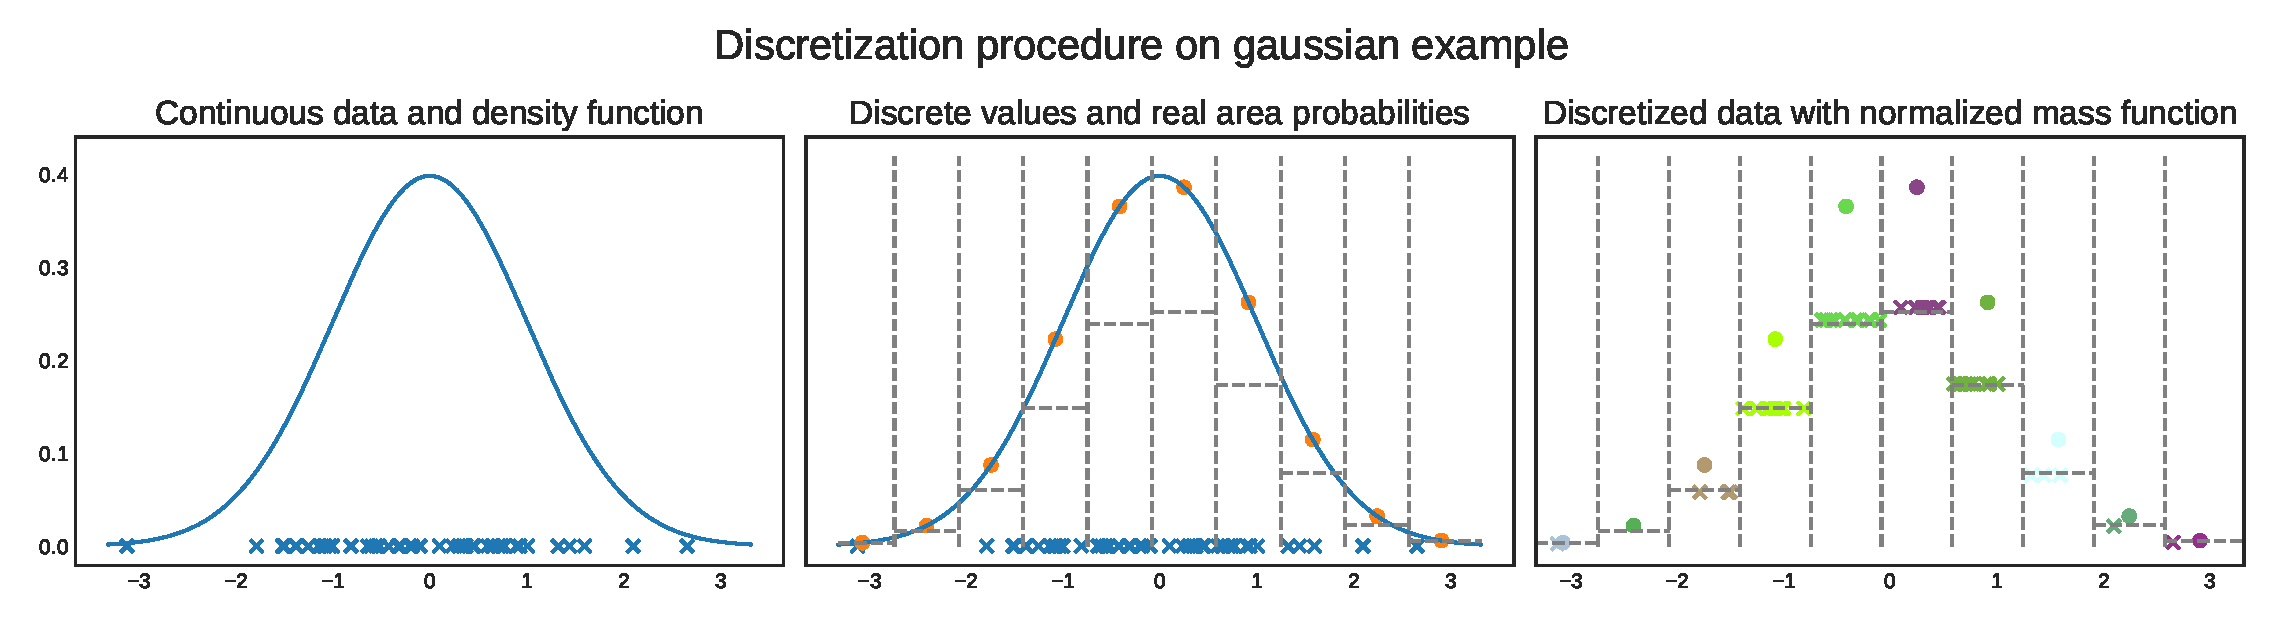
\includegraphics[scale=0.35]{discretization_image.eps}
    \caption{Illustration of the discretization process. Left: data (50 points marked with crosses) from standard normal distribution with PDF. Center: points from $\mathcal{Y^{\mathcal{D}}}$ marked on density curve (10 points in equal intervals), horizontal lines show the probabilties \linebreak $\mathbbm P (\mathcal D (y) = v^{\mathcal D})$. Right: discretized data (discrete value have been marked with colour) have been moved on the height of approximate probability $\frac{\mathbbm B(v^{\mathcal D})}{\sum_{w^{\mathcal D} \in \mathcal{Y^{\mathcal D}}} \mathbbm B(w^{\mathcal D})}$, RMSE of the probability approximation is $4.10 \cdot 10^{-3}$.}
    \label{fig:1d_discrete}
\end{figure}

In the paper \textit{Extending DenseHMM with Continuous Emission} \cite{balcerek}, authors proposed using exact probabilities instead the above approximation. It lead to good results. However, the complexity of the model increased, as some distributions do not have exact formulas for CDF (for example multivariate Gaussian with dependent coordinates). They also describe the co-occurrence for continuous observations as region-based co-occurrence. In terms of disretization technique described in this thesis, we can also consider such regions as part of the space which result in a given discrete value. 

When we decided to use approximate probabilities, the main challenge in defining a good discretization procedure is selecting $\mathcal{Y}^{\mathcal{D}}$. 


\section{$\mathcal{Y}^{\mathcal{D}}$  
discrete set selection strategies} \label{sec:discr_ys}

The strategies of selecting the discrete values can be divided into three classes:
\begin{enumerate}
    \item predefined rules (for example use equally distributed points, use points distributed as quantiles of normal distribution etc) - used originally for FlowHMM,
    \item random points (which in practise are pseudo-random points, for example randomly selected observations or points uniformly distributed at $\hat{\mathcal{Y}^{\mathcal{D}}}$),
    \item quasi-random numbers produced on $\hat{\mathcal{Y}}^{\mathcal{D}}$ (like Sobol, Halton, Latin Hypercube).
\end{enumerate}
We will discuss them in general and provide examples for further use in experiments. 

\subsection{$\mathcal{Y}^{\mathcal{D}}$ with predefined rules} \label{sec:ordinar_grid}

This group of procedures contains fixed functions transforming a hypercube $\hat{\mathcal{Y}}$ into a grid $\mathcal{Y}^{\mathcal{D}}$. In experiments we will use a grid spreading each dimension in a number of points in equal intervals. 

\begin{definition}{Ordinary grid} 

    Let us fix $M^{\mathcal  D} = \prod_{d=1}^D M_d^{\mathcal  D}$. The ordinary grid $\mathcal Y^{\mathcal D}_{OG}$ is a Cartesian product of points spread in equal intervals in each dimension:
    
    \begin{equation*}
        \mathcal Y^{\mathcal D}_{OG} = \bigotimes_{d=1}^D \Bigg\{\frac{i-1}{M_d^{\mathcal D}-1}\Big(\max(\hat{\mathcal{Y}}_d) - \min(\hat{\mathcal{Y}}_d) \Big) + \min(\hat{\mathcal{Y}}_d): i \in \mathbbm N_{\leq M_d^{\mathcal D}}^+ \Bigg\}\text{,}
    \end{equation*}
    where $\hat{\mathcal{Y}}_d$ denotes the $d$-th dimension of the hyper cube $\hat{\mathcal{Y}}$.
\end{definition}


In the model implementation we reproduce $(M_d^{\mathcal  D})_{d=1}^{D}$ from $M^{\mathcal  D}$ with the recursive procedure:

\begin{equation*}
    M_d^{\mathcal  D} =\Bigg\lfloor \sqrt[D - d + 1]{\frac{M^{\mathcal  D}}{\prod_{e=1}^{d-1} M_e^{\mathcal  D}}} \Bigg\rfloor
\end{equation*}

Using above procedure allows to use different discretization techniques with the same user interface and force the number of divisions in all dimensions to be close. 

% For simplicity, we will start to define the ordinary grid for $M = m^d$. The construction of the grid relies on the division of the range of each coordinate for m equal parts. The $(i+1)$th interval on the division of the $jth$ coordinate will be denoted as $i_j$.

% \begin{equation}
%     g_{1 + \sum_{j=1}^d i_j m^{j-1}} = \Bigg(\frac{i_j + 0.5}{m} \Big(max(V_j) - min(V_j)\Big) + min(V_j)\Bigg)_{j=1}^d
% \end{equation}

% Of course, $i_j \in \{0, 1, \ldots, m-1\}$.

% In a general case, we allow other grid sizes. However, it can happen, that the grid will be smaller than assumed (the real number of nodes will be lower than $M$). We will divide the $i$th dimension in $m_i$ intervals:

% \begin{equation} \label{eq:mi}
%     m_i =\Bigg\lfloor \sqrt[d - i + 1]{\frac{M}{\prod_{t=1}^{i-1} m_t}} \Bigg\rfloor
% \end{equation}

% Then elements of the grid can be described by the following equation:

% \begin{equation}
%     g_{1 + \sum_{j=1}^d [i_j \prod_{t=1}^{j-1}m_t]} = \Bigg(\frac{i_j + 0.5}{m_j} \Big(max(V_j) - min(V_j)\Big) + min(V_j)\Bigg)_{j=1}^d
% \end{equation}

% Of course,  $i_j \in \{0, 1, \ldots, m_j-1\}$.

% \subsection{Example: Gaussian HMM}



\subsection{$\mathcal{Y}^{\mathcal{D}}$ with (pseudo-)randomness}

When we define the random way of selecting $\mathcal{Y}^{\mathcal{D}}$ using some mathematical object, we describe something that is really random. The prefix \textit{pseudo-} refers to the implementation part. When we simulate randomness on a computer, we do deterministic operations imitating randomness and that is what we call pseudo-randomness. 

We will use three grid selection techniques. First is based on the observed data, second is based only on the data range, third is a kind of stratified sampling method. 

\begin{definition}{Random Observation Grid}

     Let us fix $M^{\mathcal  D}$. The random observation grid $\mathcal Y^{\mathcal D}_{RO}$ is an random sample of size $M$ from discrete uniform distribution $\mathcal U (y_{1:T})$.
    % \begin{equation}
    %     \mathcal Y^{\mathcal D}_{RO} 
    % \end{equation}
\end{definition}

\begin{definition}{Random Uniform Grid}

     Let us fix $M^{\mathcal  D}$. The random observation grid $\mathcal Y^{\mathcal D}_{RU}$ is an random sample of size $M$ from discrete uniform distribution $\mathcal U (\hat{\mathcal Y})$.
    % \begin{equation}
    %     \mathcal Y^{\mathcal D}_{RO} 
    % \end{equation}
\end{definition}


\begin{definition} {Latin Hypercube}

    Latin cube sampling is a stratified sampling technique. Let us fix $M$. We devide the hypercybe $\hat{\mathcal Y}$ in $M$ equal intervals in each dimension. Then we sample $\mathcal Y^{\mathcal D}_{LH}$ from $\hat{\mathcal Y}$ uniformly at random, so that looking at each dimension in each of the $M$ intervals we have only one observation. 
\end{definition}


% \section{Random Observations}

% In this case, the grid elements are just observations selected uniformly at random without repetitions. As we consider continuous emission, we can assume, that the observations do not repeat in the training set.

% $\mathbbm P (G = \{x_{i_1}, x_{i_2}, \ldots, x_{i_M}\}) = \prod_{i_1}^M \frac 1 {M - i + 1} \cdot \mathbbm 1 (\forall_{j} \forall_{t\neqj} \quad i_j \neq i_t)$


% \subsection{Example: Gaussian HMM}



% \section{Random Points from Uniform Distribution}

% This approach is similar to \ref{sec:ordinar_grid}. However, the nodes in each coordinate will be chosen uniformly. We will define a list of uniform random vectors: 
% $$\Bigg[\Big(u_{ij} \sim \mathcal U\big(min(V_j), max(V_j)\big)\Big)i=1^m_j\Bigg]_{j=1}^d$$

% Then the grid elements can be described as:

% \begin{equation}
%     g_{1 + \sum_{j=1}^d [i_j \prod_{t=1}^{j-1}m_t]} = \big(u_{i_j, j}\big)_{j=1}^d
% \end{equation}

% \subsection{Example: Gaussian HMM}



\subsection{$\mathcal{Y}^{\mathcal{D}}$ with quasi-randomness}

Quasi-random numbers differ from pseudo-random numbers. Pseudo-random numbers are designed to imitate randomness while quasi-random numbers are designed to be spread evently on the space with a sense of randomness. In general, qusia-random points rarely form concentrations or blank spaces. 



\begin{definition} {Sobol Quasi-Random Numbers}

    Let us fix $M^{\mathcal  D}=2^k$. When sampling $M^{\mathcal  D}$ $D$-dimensional points from a Sobol sequence, we actually sample $D$ sequences of length $M^{\mathcal  D}$.
    
    \begin{equation*}
        y^{\mathcal D}_{d, m} = \sum_{j=0}^{k-1} a_j \frac{\mathcal{DN}_{d, j}}{2^{32}}  \cdot  (max (\hat{\mathcal{Y}}_d)  - min(\hat{\mathcal{Y}}_d))  + min(\hat{\mathcal{Y}}_d)
    \end{equation*}

    where $a_j$ is either $0$ or $1$ and it flicks every $2j+1$ points, $\mathcal{DN}_{d, j}$ are 32 direction numbers.  
    % such that:
    % \begin{equation}
    %     \mathcal{DN}_{0, j} = 2^{31-j}
    % \end{equation}
     We get the sequence $\mathcal Y ^{\mathcal D}_{QS}$.
\end{definition}


\begin{definition} {Halton Quasi-Random Numbers}

    Let us fix $M^{\mathcal  D}$. Let us also fix $D$ coprime numbers $(p_d)_{d=1}^D$. Let us devide recursively the $d$-th dimension in $p_d$ intervals (and then divide each interval in $p_d$ intervals, and so on). Let us collect the intervals separating points (after scaling as $y \rightarrow y \cdot  (max (\hat{\mathcal{Y}}_d)  - min(\hat{\mathcal{Y}}_d))  + min(\hat{\mathcal{Y}}_d)$) into a sequence  $y^{\mathcal D}_{d, .}$.  Doing so for each dimension, until we become $M$ separating points,  we get the sequence $\mathcal Y ^{\mathcal D}_{QH}$.
    
\end{definition}

More information about quasi-random numbers can be found in \cite{quasi_random}. 

\section{Toy Experiment: estimating $\pi$ with a sample from $[0, 1]^2$}

In this mini-experiment,  we show the properties of sequences defined above in the task of integration of a  one dimensional function.  

We will consider $f: [0, 1] \rightarrow \mathbbm R$, $f(x) =  \sqrt{1 - x^2}$. Integrating this function can be used for calculating $\pi$:

\begin{equation} \label{eq:toy_pi}
    \pi = 4 \cdot \int_0^1 f(x) dx
\end{equation}

We will estimate the integral in two ways:

\begin{itemize}
    \item Sample 1-dimensional points, calculate the function values for those arguments and the mean of them. 
    \item Sample 2-dimensional points and calculate the ration of points in the area under the curve.  
\end{itemize}


\subsection{Estimate $\pi$ from 1D points}

Let $X$ be a random variable taking values from $[0,  1]$. We will use $R$ replications of the random variable $X$: $X_1,  \ldots, X_R$. Using those points, we can estimate $\pi$ with the formula:

\begin{equation*}
    \hat{\pi}^{1D} =  4 \cdot \frac 1 R \sum_{r=1}^R \sqrt{1 - X_r^2}\text{.}
\end{equation*}

We repeat the experiment several times, to estimate the bias and the variance of the estimator $ \hat{\pi}^{1D}$. 

\textbf{Setup:}
\begin{itemize}
    \item $R=2^6$,
    \item we  will provide several estimators using differently sourced $X$:
    \begin{itemize}
        \item $\hat{\pi}^{1D}_{OG}$ -- $X$ from ordinary grid 
        \item $\hat{\pi}^{1D}_{RO}$ -- $X$ from random observation grid 
        \item $\hat{\pi}^{1D}_{RU}$ -- $X$ from random uniform ($\mathcal U (\hat{\mathcal Y})$) grid 
        \item $\hat{\pi}^{1D}_{LH}$ -- $X$ from latin hypercube sampled grid 
        \item $\hat{\pi}^{1D}_{QS}$ -- $X$ from quasi-random Sobol grid 
        \item $\hat{\pi}^{1D}_{QH}$ -- $X$ from quasi-random Halton grid 
    \end{itemize}
    \item repeat 100 times to see the results accuracy and variability.
\end{itemize}

\textbf{Goal:}

Compare the quality of results in the integrating task for various point selection techniques. 

\textbf{Results:}

Sobol quasi random ($QS$) sequence and the latin hypercube ($LH$) performed best.  Very high bias has been obtained from the grid sample ($OG$), while the random sample ($RU$) had  very high deviation. 

\begin{figure}[!ht]
    \centering
    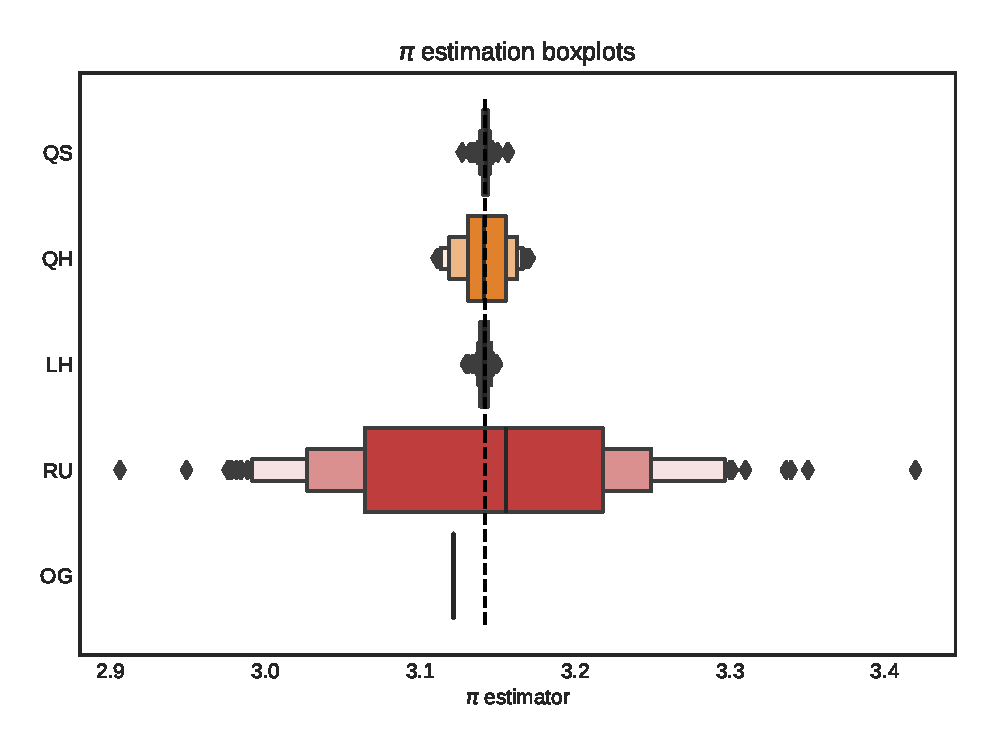
\includegraphics[scale=0.65]{pi_example_1d.eps}
    \caption{Estimator of $\pi$ with 64 points, 100 repetitions. The dashed line represents the true value of $\pi$.}
    \label{fig:toy:res}
\end{figure}

\newpage

\begin{figure}[!ht]
    \centering
    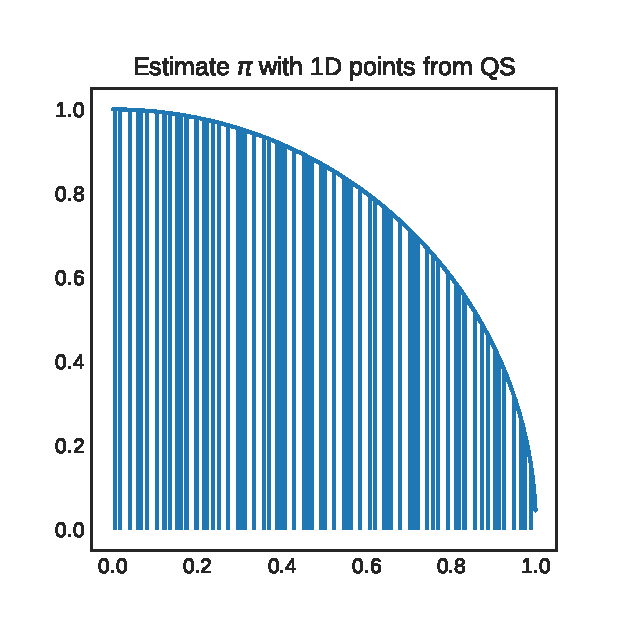
\includegraphics[scale=.6]{QS_1D_circle.eps}
    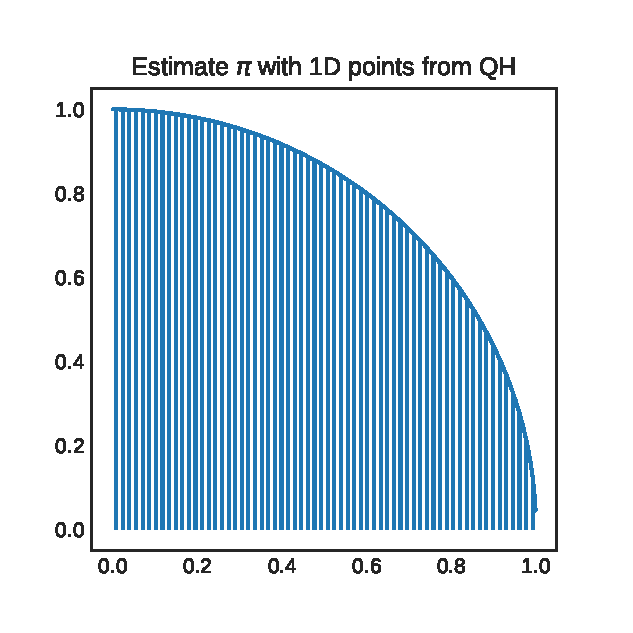
\includegraphics[scale=.6]{QH_1D_circle.eps}
    
    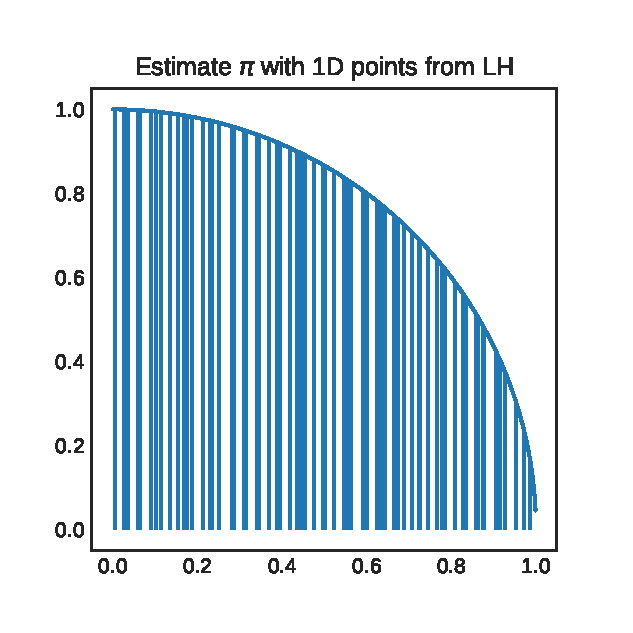
\includegraphics[scale=.6]{LH_1D_circle.eps}
    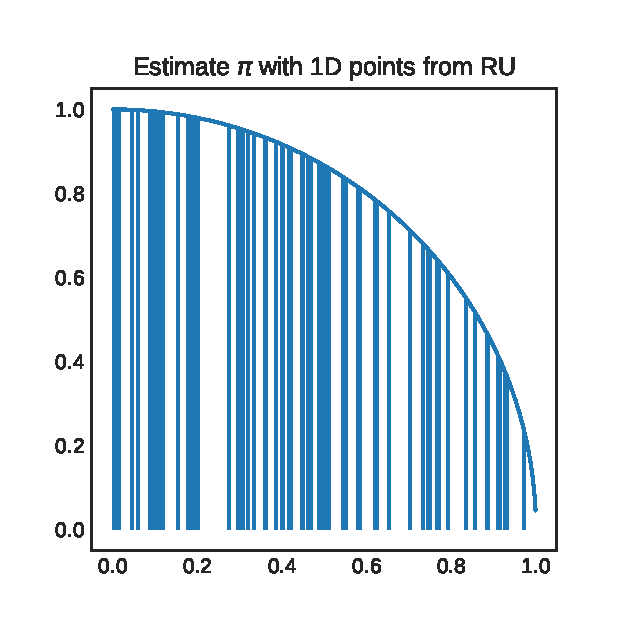
\includegraphics[scale=.6]{RU_1D_circle.eps}
    
    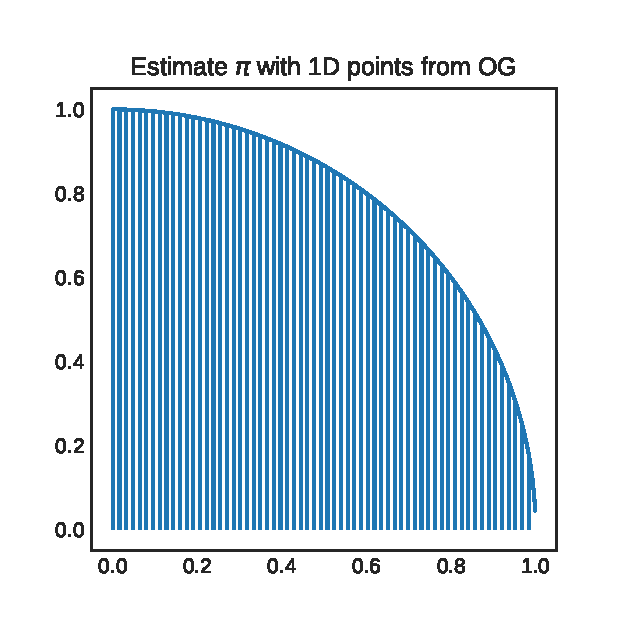
\includegraphics[scale=.6]{OG_1D_circle.eps}
    \caption{64 1D points for integral estimation.}
    \label{fig:toy-points2}
\end{figure}





\newpage

\subsection{Estimate $\pi$ from 2D points}


Let $X$ be a random variable taking values from $[0,  1]^2$. We will use $R$ replications of the random variable $X$: $X_1,  \ldots, X_R$. Using those points, we can estimate $\pi$ with the formula:

\begin{equation*}
    \hat{\pi}^{2D} =  4 \cdot \frac 1 R \sum_{r=1}^R \mathbbm 1 (X_{r,  1}^2 + X_{r,  2}^2 \leq 1)\text{,}
\end{equation*}
where $X_{r,  1}^2, X_{r,  2}$ are the first and the second coordinate of $X_r$.


We repeat the experiment several times, to estimate the bias and the variance of the estimator $ \hat{\pi}^{2D}$. 

\textbf{Setup:}
\begin{itemize}
    \item $R=2^8$,
    \item we  will provide several estimators using differently sourced $X$:
    \begin{itemize}
        \item $\hat{\pi}^{2D}_{OG}$ -- $X$ from ordinary grid 
        \item $\hat{\pi}^{2D}_{RO}$ -- $X$ from random observation grid 
        \item $\hat{\pi}^{2D}_{RU}$ -- $X$ from random uniform ($\mathcal U (\hat{\mathcal Y})$) grid 
        \item $\hat{\pi}^{2D}_{LH}$ -- $X$ from latin hypercube sampled grid 
        \item $\hat{\pi}^{2D}_{QS}$ -- $X$ from quasi-random Sobol grid 
        \item $\hat{\pi}^{2D}_{QH}$ -- $X$ from quasi-random Halton grid 
    \end{itemize}
    \item repeat 100 times to see the results accuracy and variability.
\end{itemize}

\textbf{Goal:}

Compare the quality of results in the integrating task for various point selection techniques. 

\textbf{Results:}

Quasi random samples ($QH$, $QS$) performed best both in terms of the bias and variance. The random samples ($LH$, $RU$) had high variance, the ordinary grid had high bias.  Looking at the results of both variant of the experiment, the quasi random numbers seem to work best in the integration task.

\begin{figure}[!ht]
    \centering
    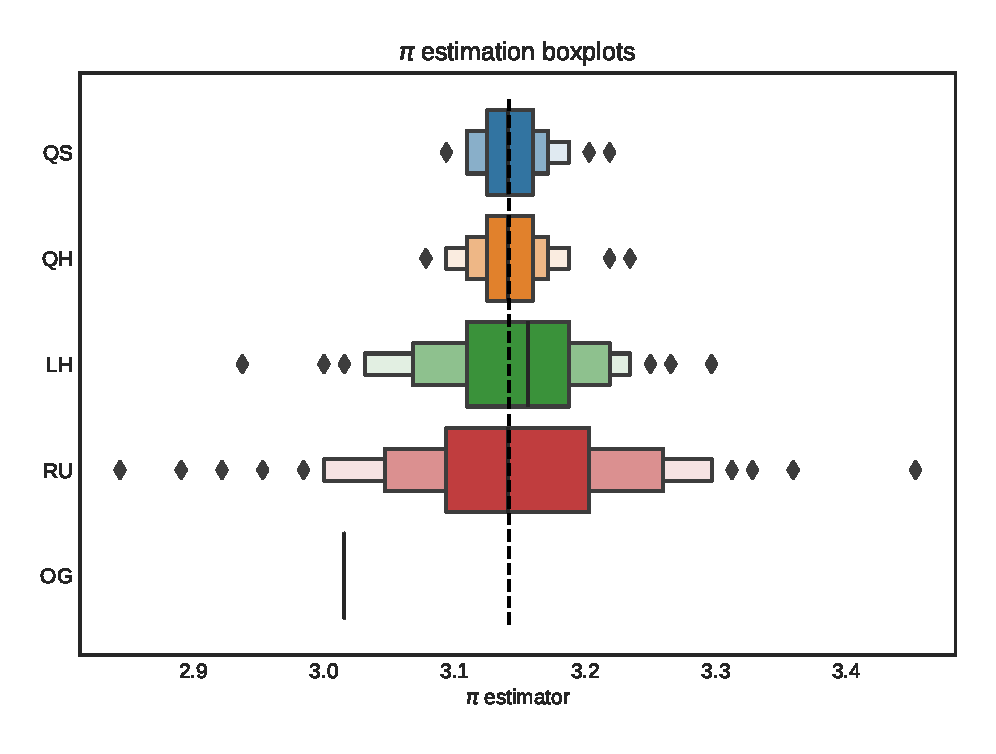
\includegraphics[scale=0.65]{pi_example_2d.eps}
    \caption{Estimator of $\pi$ with 256 points, 100 repetitions. The dashed line represents the true value of $\pi$.}
    \label{fig:toy:res}
\end{figure}

\newpage

\begin{figure}[!ht]
    \centering
    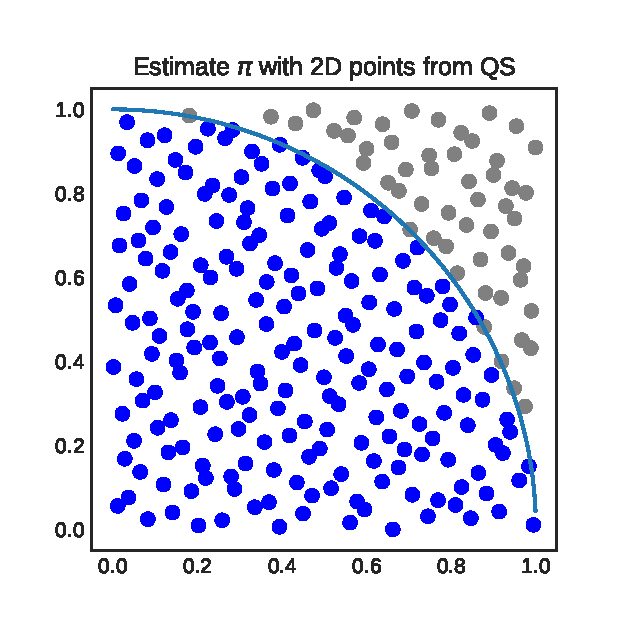
\includegraphics[scale=.6]{QS_2D_circle.eps}
    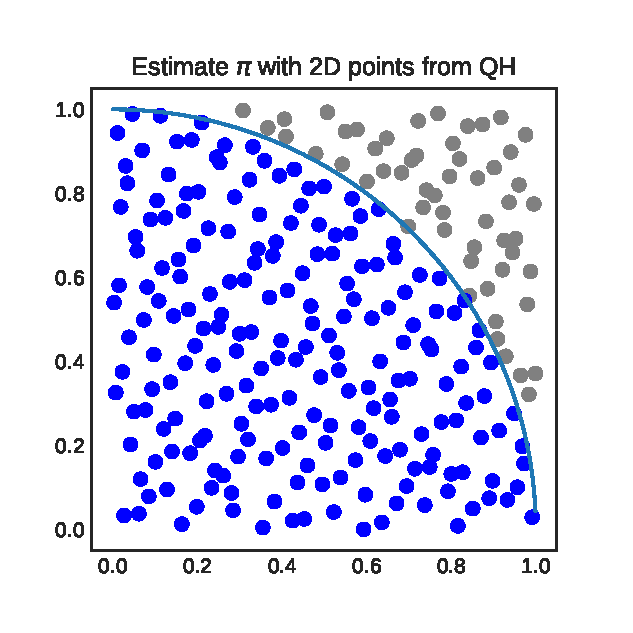
\includegraphics[scale=.6]{QH_2D_circle.eps}

    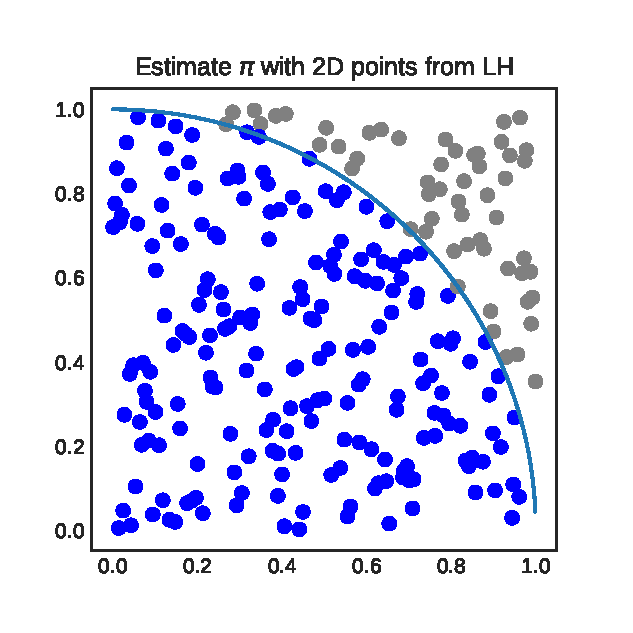
\includegraphics[scale=.6]{LH_2D_circle.eps}
    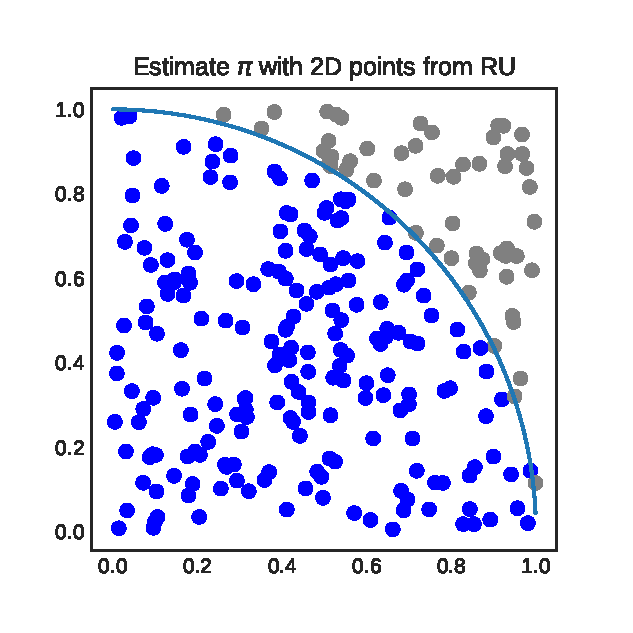
\includegraphics[scale=.6]{RU_2D_circle.eps}
    
    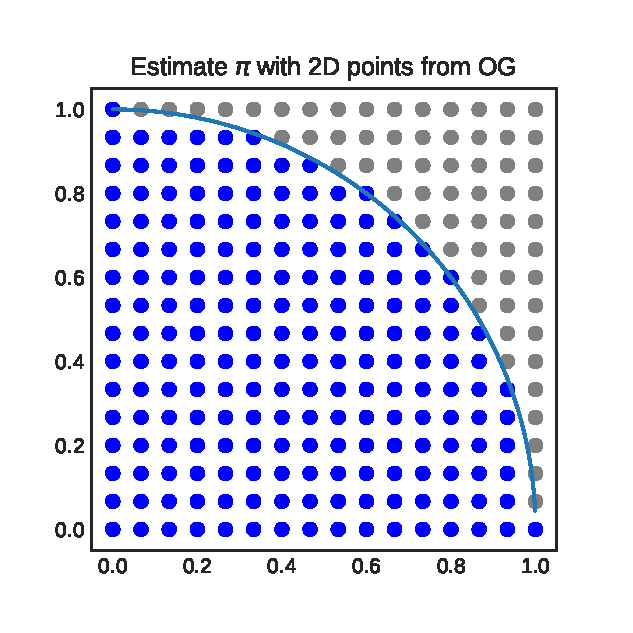
\includegraphics[scale=.6]{OG_2D_circle.eps}
    \caption{256 2D points for integral estimation.}
    \label{fig:toy-points2}
\end{figure}

\newpage

% The results of 100 runs of the experiments are shown in Figure \ref{fig:toy:res}. The best results for 2D method  have been obtained for quasi-random points. They had low variance and low bias. The random techniques had a very high variance (stratified technique - latin cube - had lower variance that uniform but still higher than quasi-random techniques and furthermore it was biased) while the ordinary 2d grid had a high bias (with zero variance as the technique is fully deterministic). One dimensional points gave better results: deterministic points were almost ideal, uniform 1D points got better than the 2D variant.  What  is interesting: 1D uniform worked worse than 2D Sobol and Halton (even if it had exact function values given). 


\section{Example: GaussianHMM}

In this example we show the influence of discretization  on a sample from Gaussian HMM.

\subsection{GaussianHMM with 2D emission}

\textbf{Setup:}

\begin{itemize}
    \item $T = 100$ - sequence length,
    \item $M = 16$ - number of  discrete values,
    \item we provide the set of discrete values and calculate the negative log-likelihood of the discretized sequence (in original model),
    \item repeat the experiment 100 times.
\end{itemize}

\textbf{Goal:}

Compare the likelihood of  discretized  (with various approaches) sequence to the original one. 

\textbf{Results:}

Figure \ref{fig:gaussian-hmm-nodes} shows the sequence with different discretization variants.  Figure \ref{fig:gaussian-hmm-discrete-res} presents the experiment results summary. 

The worst results were obtained with an ordinary grid (no variance but immense bias). In this experiment, the results obtained via lating hypercube ($LH$), uniform distribution ($RU$) and quasi-random sequences ($QS$, $QH$) seem to be comparable. Halton ($QH$) works best out of this three. A surprising part of the experiment is that we can obtain even better results than the original sequence when we use the random observation grid ($RO$). This is probably because  we are more likely to select a point close to the mean value (and replace the more distant ones with it in the discretization procedure) than a distant from mean point (which are most probably just rare in the sample). My main concern with this method is that it can miss the distant and less common part of the observation space. This in some cases can result in a huge error in the further training of the model. Also quantile latin hypercube ($LC_q$) performed a bit better than the techniques independent from the data. However, it is not feasible in many cases (it  is to costly to calculate the quantiles for  large data sets). 

\pagebreak

\begin{figure}[!ht]
    \centering
    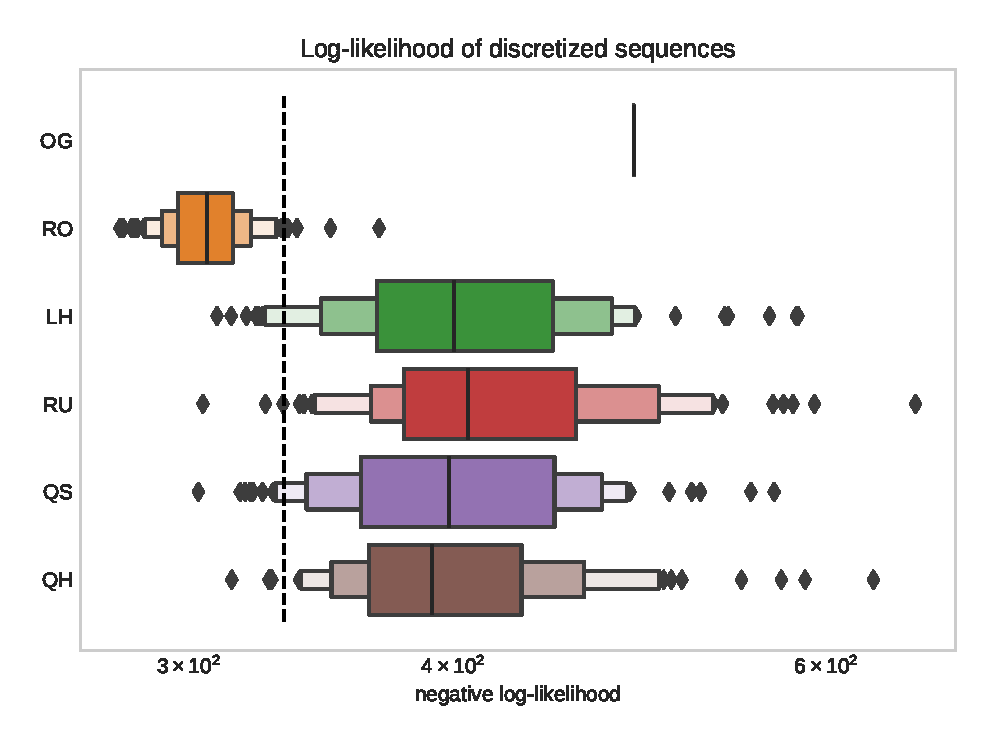
\includegraphics[scale=0.65]{gaussianHMM_example.eps}
    \caption{Negative log-likelihood of  discretized sequence. The horizontal line shows the score for original sequence.}
    \label{fig:gaussian-hmm-discrete-res}
\end{figure}

\newpage

\begin{figure}[!ht]
    \centering
    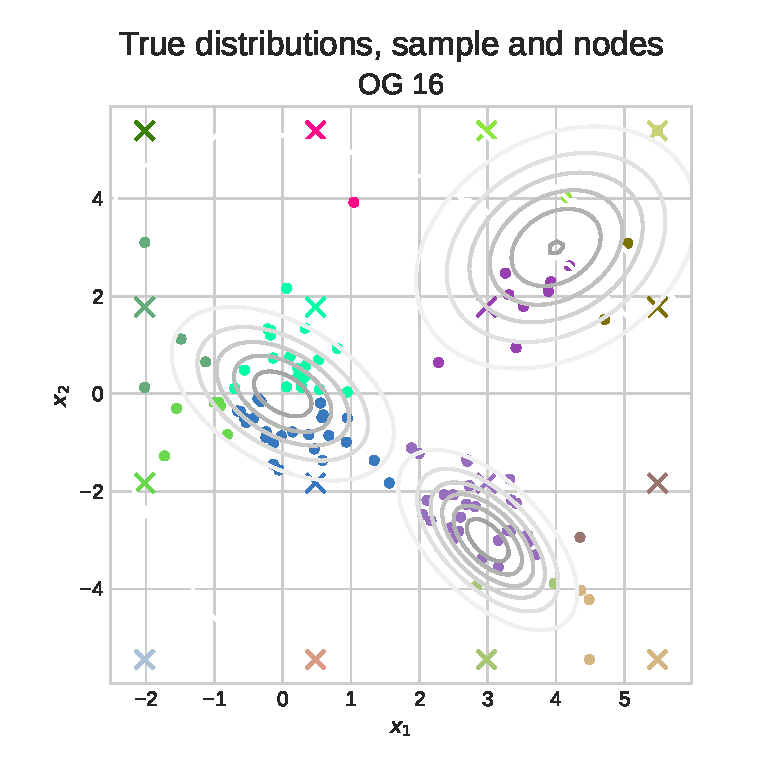
\includegraphics[scale=0.42]{gaussianHmm_discrete_example_grid.eps}
    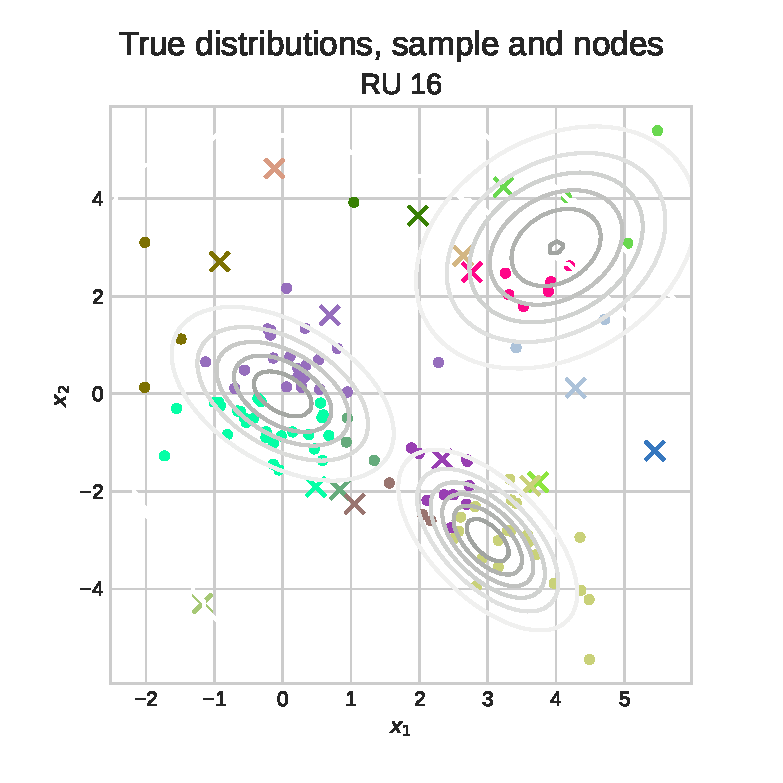
\includegraphics[scale=0.42]{gaussianHmm_discrete_example_uniform.eps}
    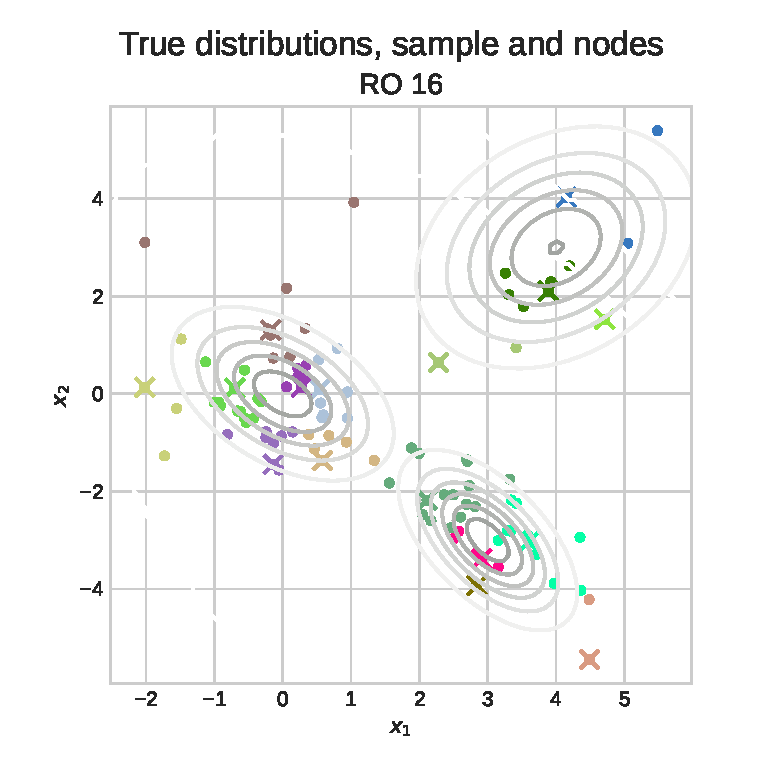
\includegraphics[scale=0.42]{gaussianHmm_discrete_example_random.eps}
    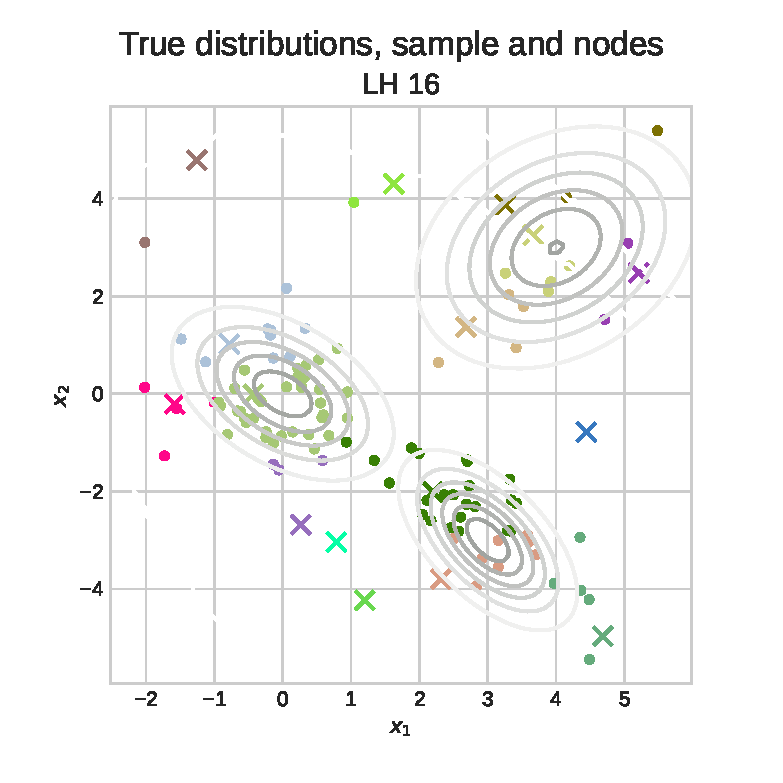
\includegraphics[scale=0.42]{gaussianHmm_discrete_example_latin_cube_u.eps}
    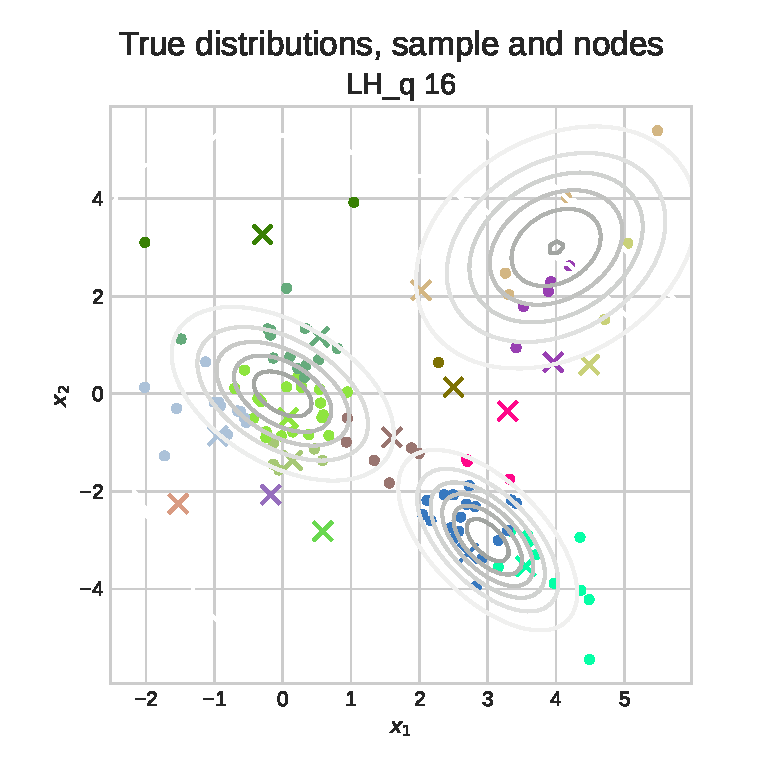
\includegraphics[scale=0.42]{gaussianHmm_discrete_example_latin_cube_q.eps}
    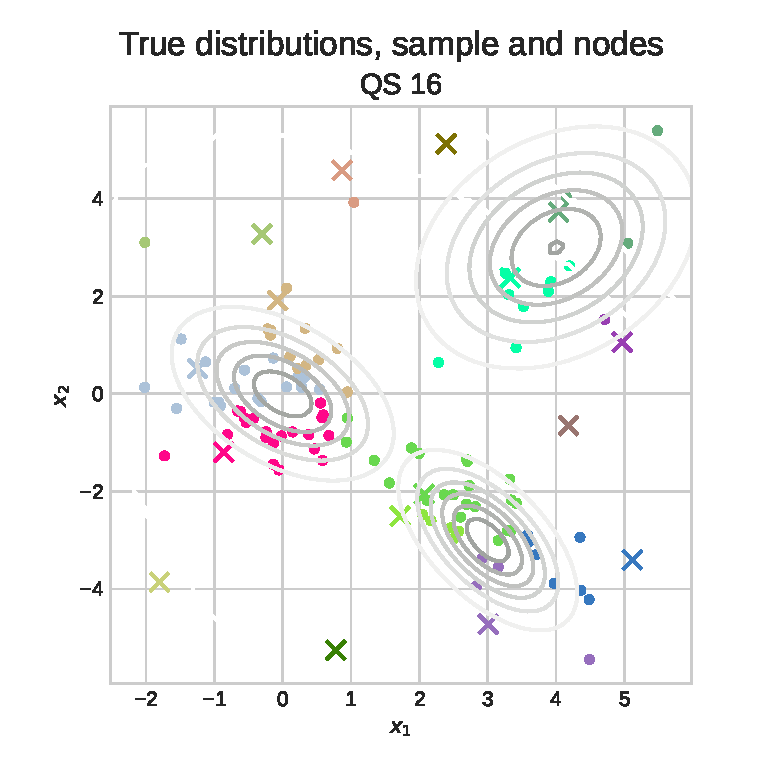
\includegraphics[scale=0.42]{gaussianHmm_discrete_example_sobol.eps}
    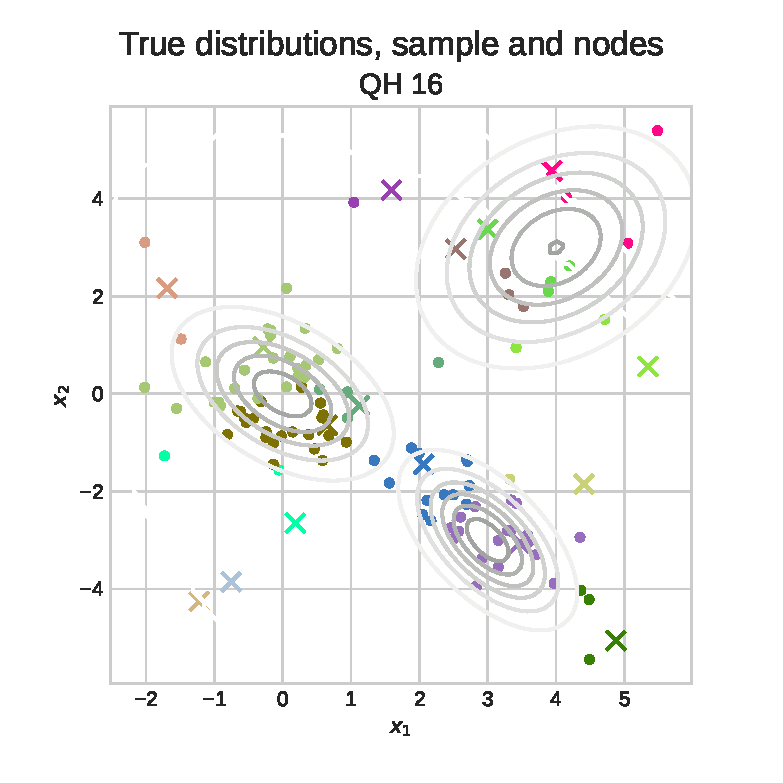
\includegraphics[scale=0.42]{gaussianHmm_discrete_example_halton.eps}
    \caption{A 100-element long sequence from Gaussian HMM (points) with true distribution (grey elipses), 16 discrete nodes (crosses), and discretization marked as colour of the closest discrete value.}
    \label{fig:gaussian-hmm-nodes}
\end{figure}

\newpage


% \begin{figure}[!h]
%     \centering
%     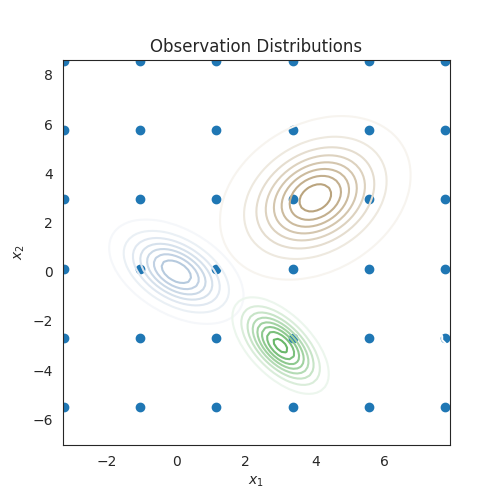
\includegraphics[scale=0.4]{1_nodes_grid_39_v2.png}
%     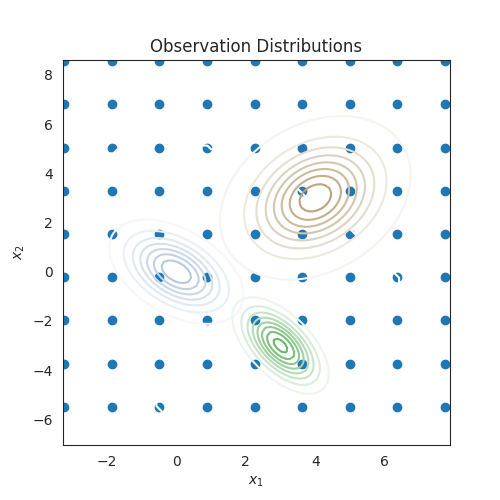
\includegraphics[scale=0.4]{1_nodes_grid_83_v2.png}
%     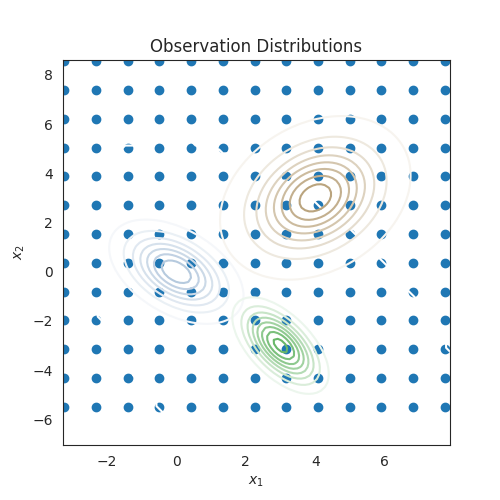
\includegraphics[scale=0.4]{1_nodes_grid_174_v2.png}
%     \caption{Caption}
%     %\label{fig:enter-label}
% \end{figure}

% \begin{figure}[!h]
%     \centering
%     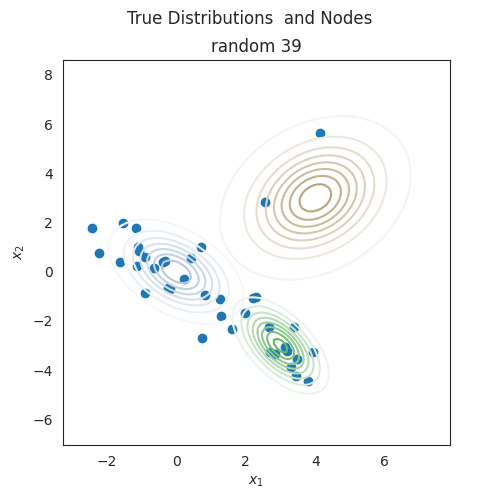
\includegraphics[scale=0.4]{1_nodes_random_39_v2.png}
%     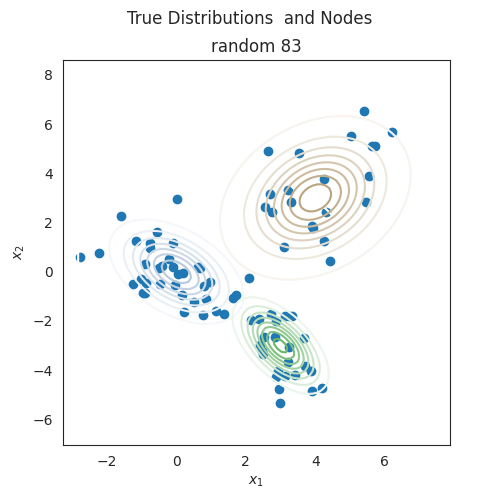
\includegraphics[scale=0.4]{1_nodes_random_83_v2.png}
%     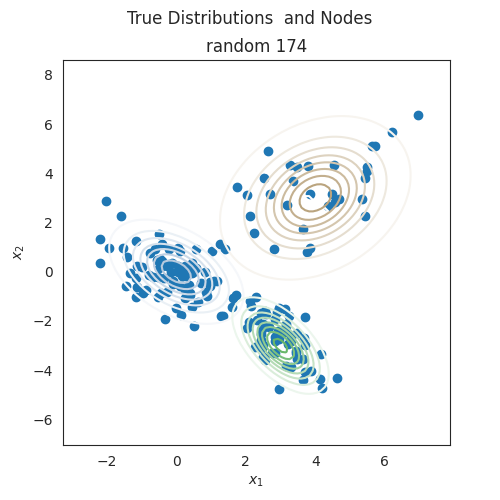
\includegraphics[scale=0.4]{1_nodes_random_174_v2.png}
%     \caption{Caption}
%     %\label{fig:enter-label}
% \end{figure}

% \begin{figure}[!h]
%     \centering
%     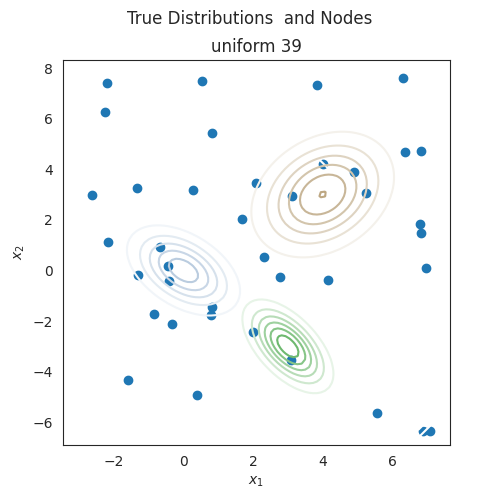
\includegraphics[scale=0.4]{1_nodes_uniform_39_v2.png}
%     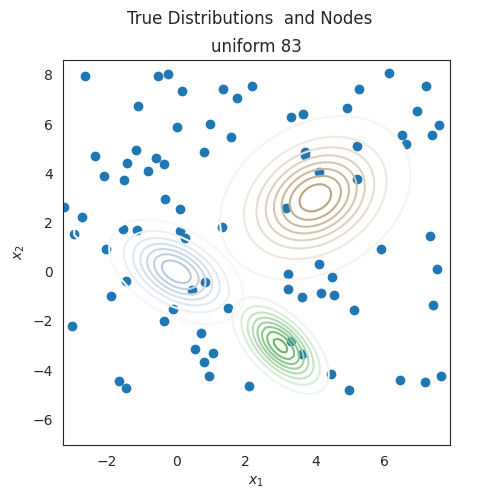
\includegraphics[scale=0.4]{1_nodes_uniform_83_v2.png}
%     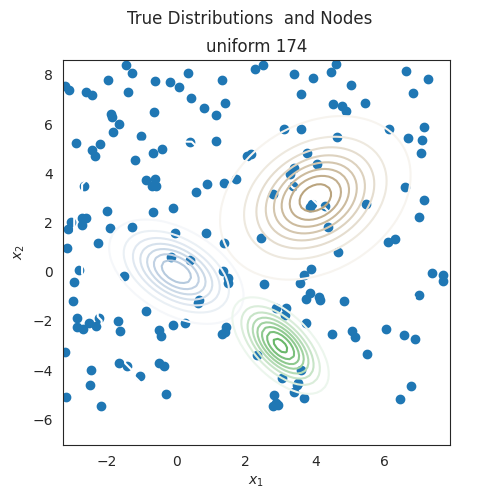
\includegraphics[scale=0.4]{1_nodes_uniform_174_v2.png}
%     \caption{Caption}
%     %\label{fig:enter-label}
% \end{figure}

% \begin{figure}[!h]
%     \centering
%     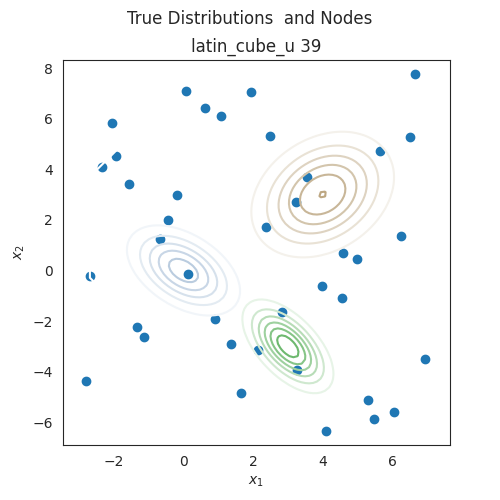
\includegraphics[scale=0.4]{1_nodes_latin_cube_u_39_v2.png}
%     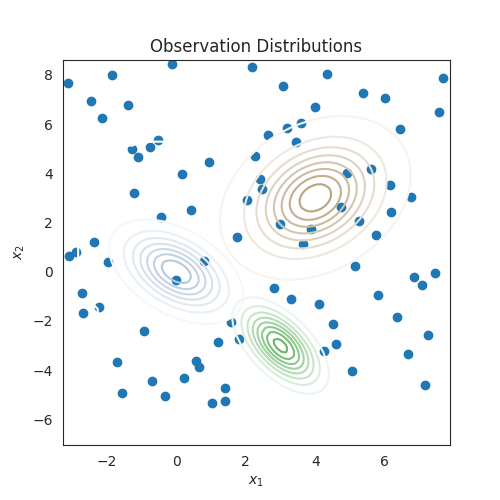
\includegraphics[scale=0.4]{1_nodes_latin_cube_u_83_v2.png}
%     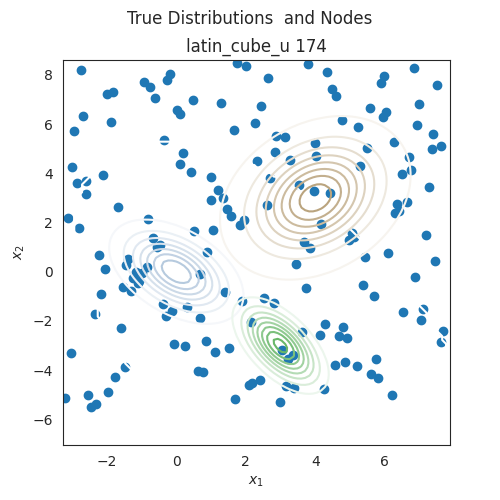
\includegraphics[scale=0.4]{1_nodes_latin_cube_u_174_v2.png}
%     \caption{Caption}
%     %\label{fig:enter-label}
% \end{figure}

% \begin{figure}[!h]
%     \centering
%     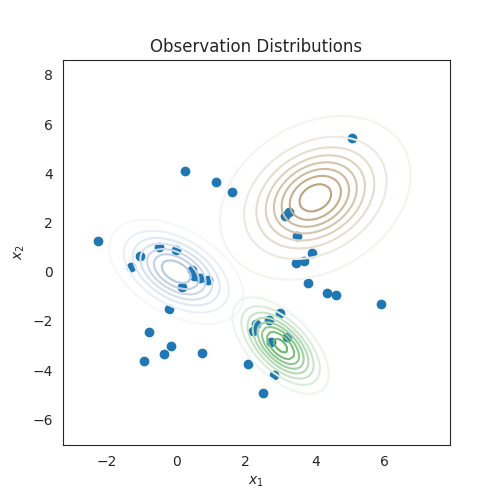
\includegraphics[scale=0.4]{1_nodes_latin_cube_q_39_v2.png}
%     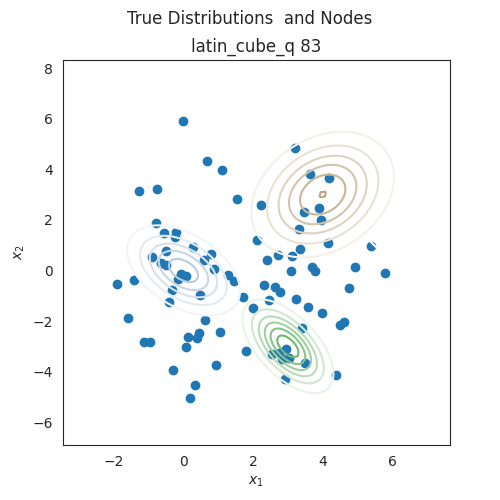
\includegraphics[scale=0.4]{1_nodes_latin_cube_q_83_v2.png}
%     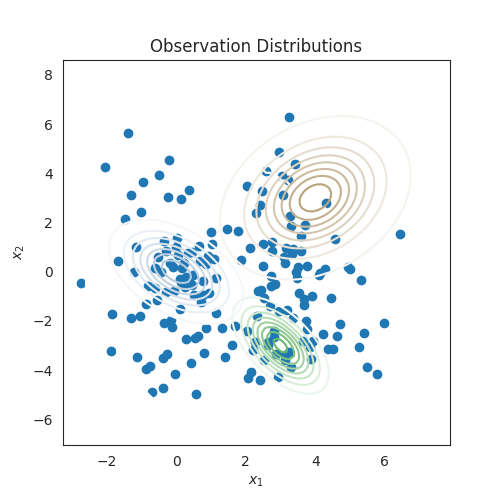
\includegraphics[scale=0.4]{1_nodes_latin_cube_q_174_v2.png}
%     \caption{Caption}
%     %\label{fig:enter-label}
% \end{figure}



% \begin{figure}[!h]
%     \centering
%     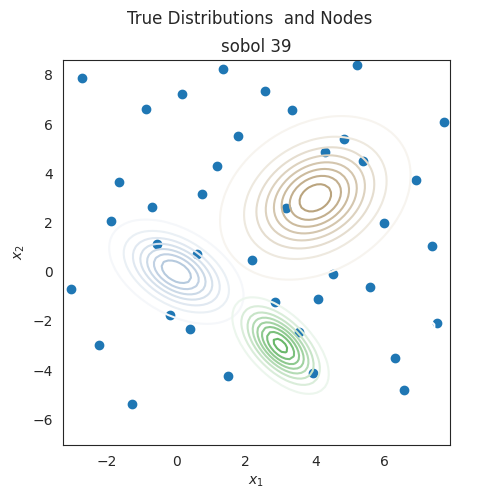
\includegraphics[scale=0.4]{1_nodes_sobol_39_v2.png}
%     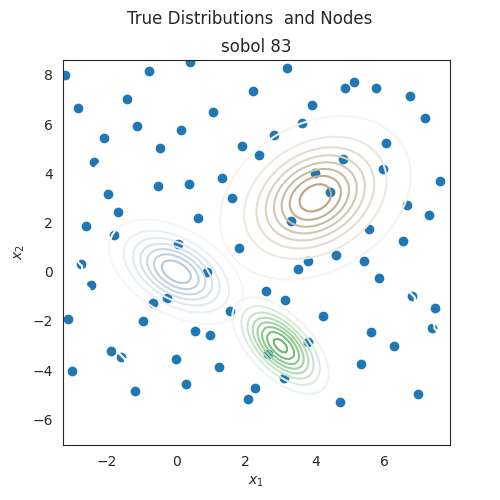
\includegraphics[scale=0.4]{1_nodes_sobol_83_v2.png}
%     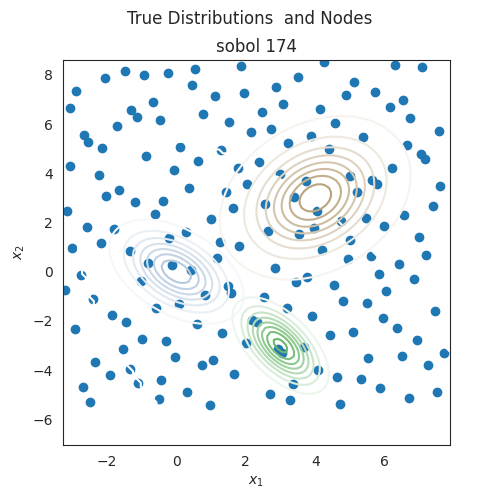
\includegraphics[scale=0.4]{1_nodes_sobol_174_v2.png}
%     \caption{Caption}
%     %\label{fig:enter-label}
% \end{figure}



% \begin{figure}[!h]
%     \centering
%     \includegraphics[scale=0.4]{1_nodes_QH_39_v2.png}
%     \includegraphics[scale=0.4]{1_nodes_QH_83_v2.png}
%     \includegraphics[scale=0.4]{1_nodes_QH_174_v2.png}
%     \caption{Caption}
%     %\label{fig:enter-label}
% \end{figure}

\subsection{GaussianHMM with 10D emission} \label{sec:ex_gauss_10d}

\textbf{Setup:}
\begin{itemize}
    \item $T = 2000$ - sequence length,
    \item $M = 256$ - number of  discrete values,
    \item we provide the set of discrete values and calculate the negative log-likelihood of the discretized sequence (in original model),
    \item repeat the experiment 100 times,
    \item means for the experiment were sampled from $\mathcal U[-5,  5]$,
    \item covariance matrices were obtained from the Cholesky decomposition, we generated a lower triangular matrices from $\mathcal U[0.1,  1.1]$.
\end{itemize}

\textbf{Goal:}

Compare the likelihood of  discretized  (with various approaches) sequence to the original one. 

\textbf{Results:}

The conclusions could be the same as for the 2D version of the experiment. 


\begin{figure}[!ht]
    \centering
    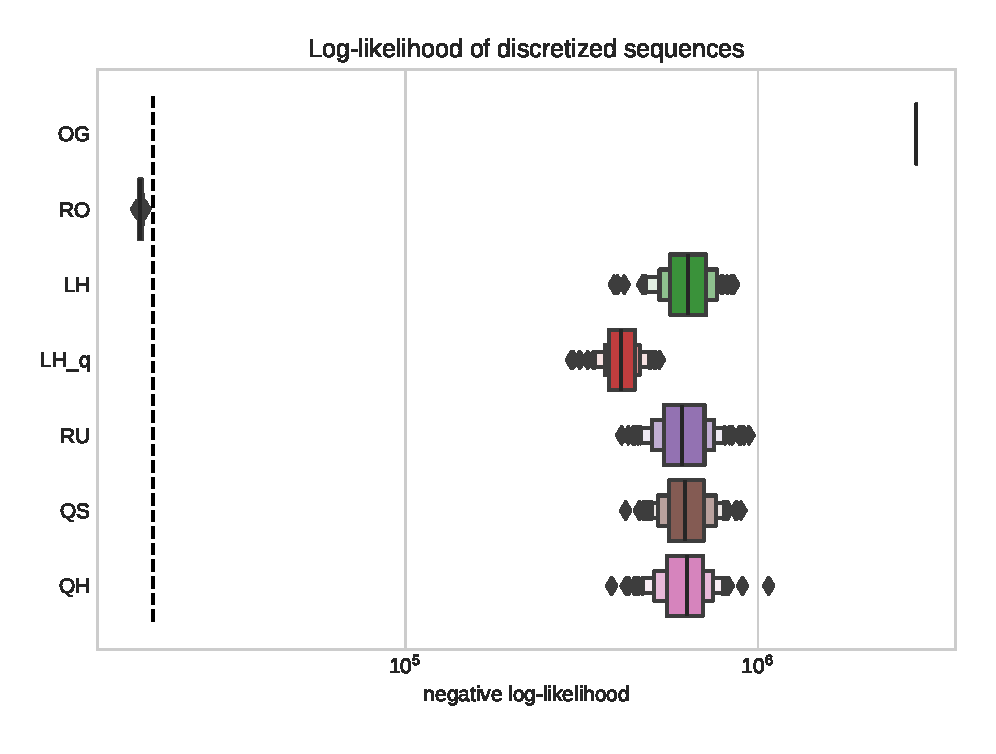
\includegraphics[scale=0.65]{10d_gaussianHMM_example.eps}
    \caption{Negative log-likelihood of  discretized sequence. The horizontal line shows the score for original sequence.}
    \label{fig:gaussian-hmm-discrete-res}
\end{figure}

\pagebreak
\begin{figure}[!h]
    \centering
    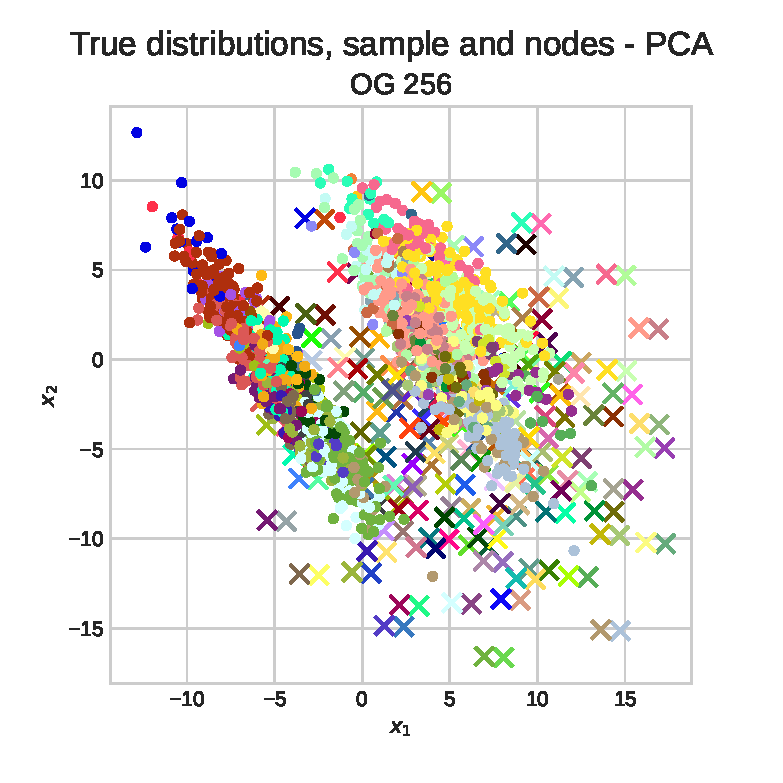
\includegraphics[scale=0.42]{10d_gaussianHmm_discrete_example_grid.eps}
    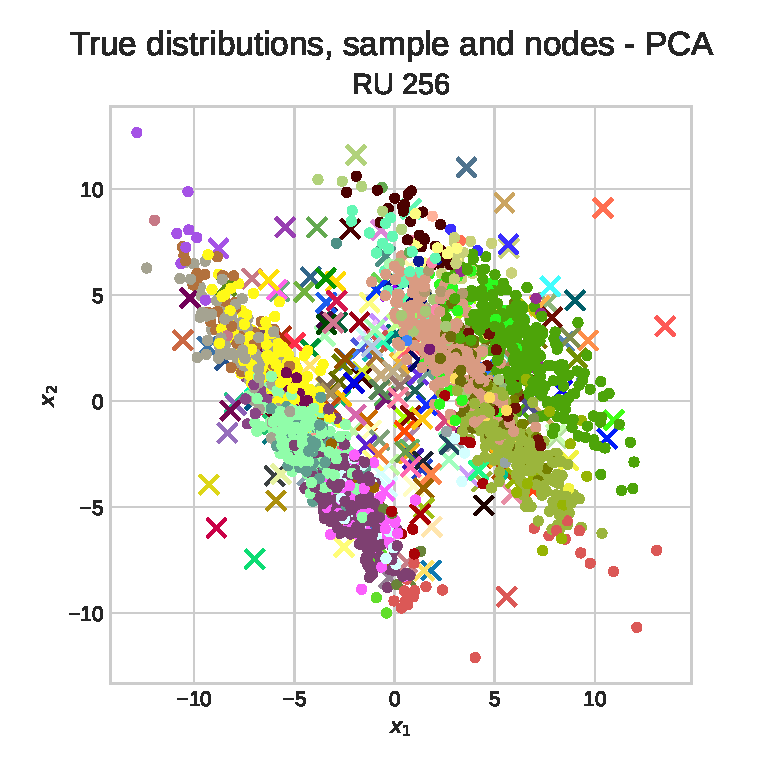
\includegraphics[scale=0.42]{10d_gaussianHmm_discrete_example_uniform.eps}
    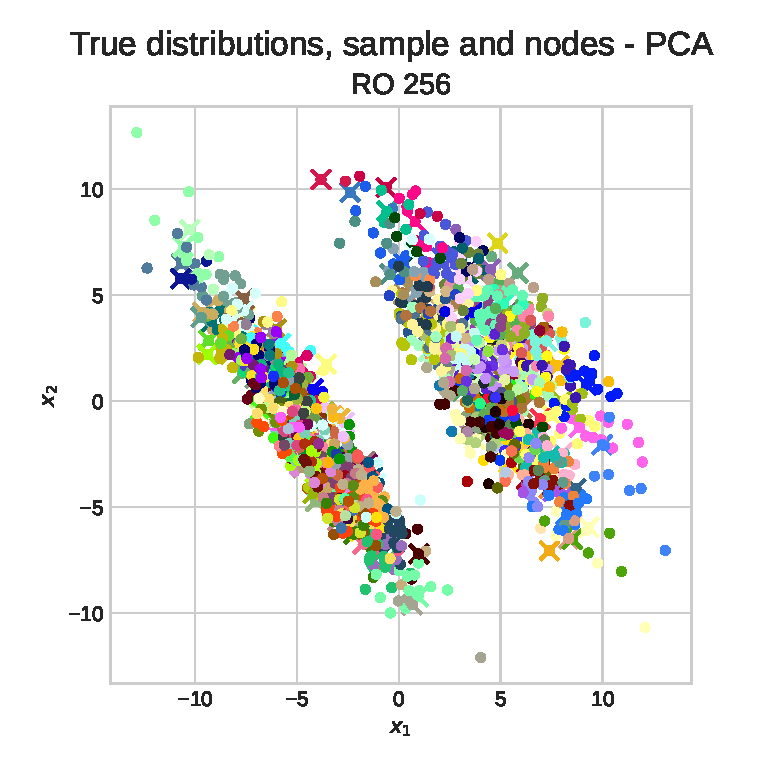
\includegraphics[scale=0.42]{10d_gaussianHmm_discrete_example_random.eps}
    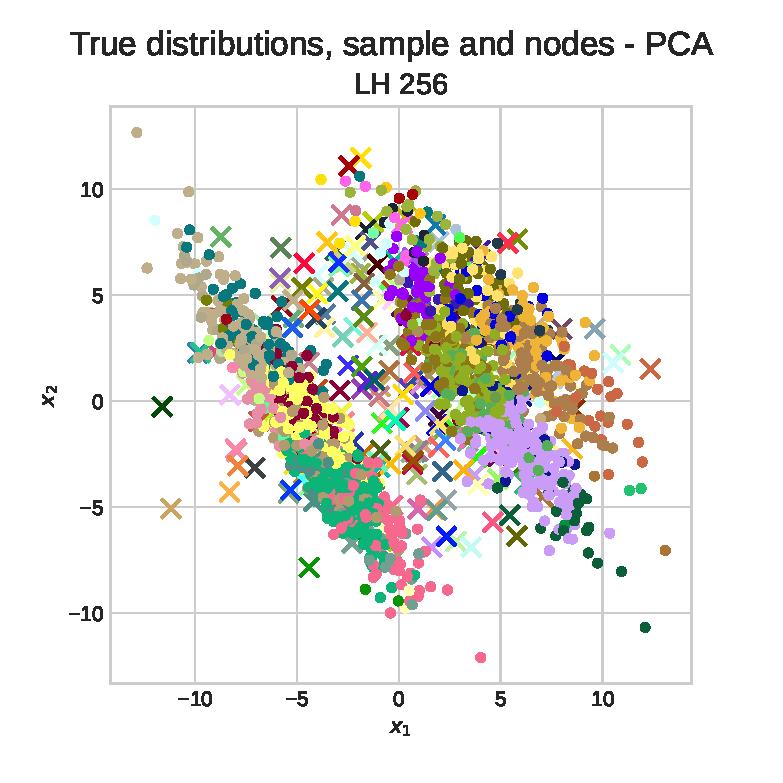
\includegraphics[scale=0.42]{10d_gaussianHmm_discrete_example_latin_cube_u.eps}
    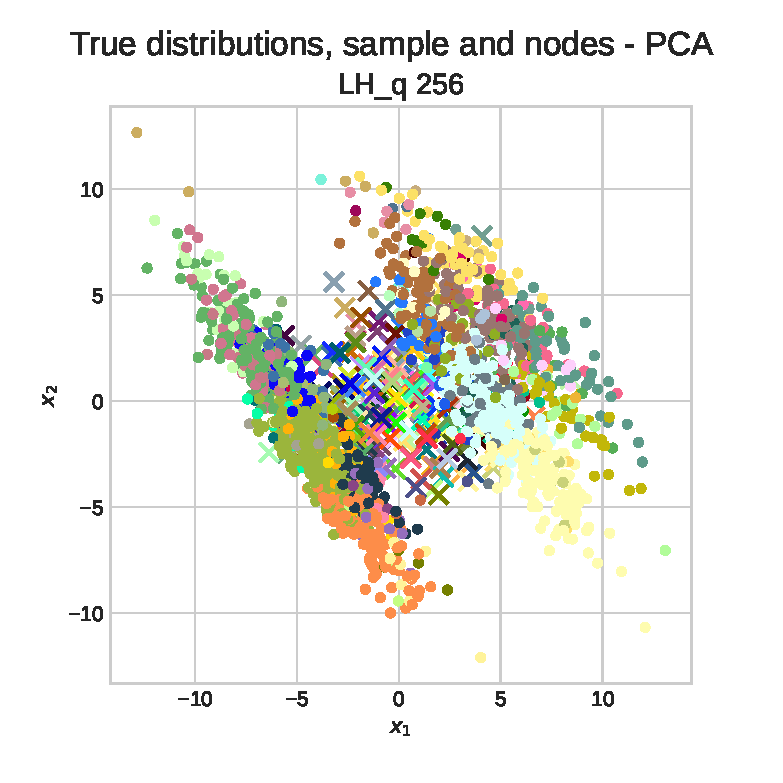
\includegraphics[scale=0.42]{10d_gaussianHmm_discrete_example_latin_cube_q.eps}
    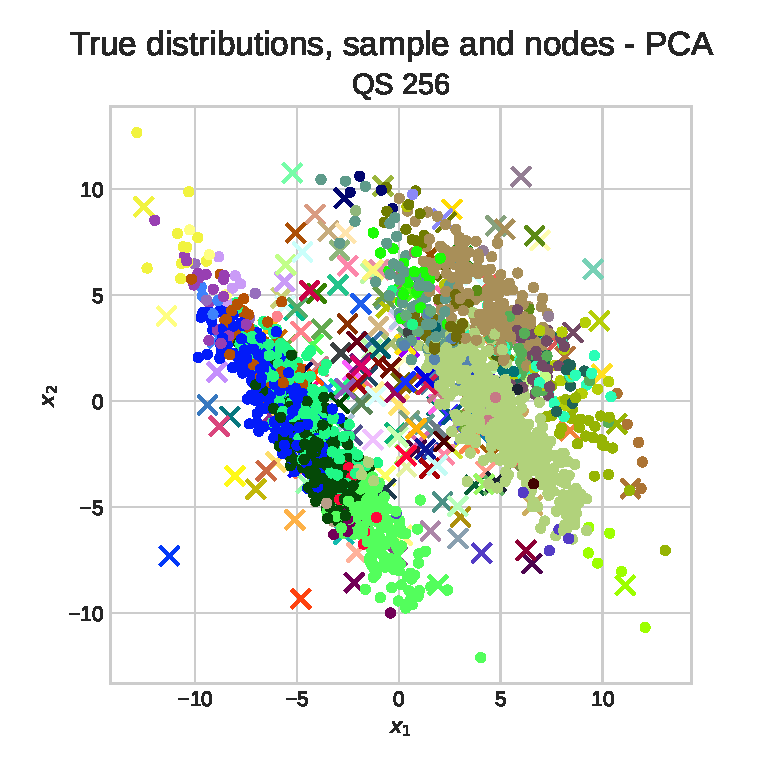
\includegraphics[scale=0.42]{10d_gaussianHmm_discrete_example_sobol.eps}
    \includegraphics[scale=0.42]{10d_gaussianHmm_discrete_example_halton.eps}
    \caption{A 2000-element long sequence from Gaussian HMM (points) with true distribution (grey elipses), 256 discrete nodes (crosses), and discretization marked as colour of the closest discrete value.}
    \label{fig:gaussian-hmm-nodes}
\end{figure}
\pagebreak




\pagebreak

\chapter{Modern approach: Flow HMM} \label{sec:flowhmm}

As it was mentioned in Chapter \ref{sec:limitations}, one of the most recently proposed extensions of the Hidden Markov Model is the FlowHMM by Lorek et al. \cite{lorek2022flowhmm}. The authors address the issue  that the emission distribution must come from a parametrized family. They propose to model the emission for each state with a normalizing flow neural network. In this chapter, we will present this component of the modern model and compare it to the traditional solution. 


\section{Normalizing Flow}

In this section, we will consider $Y$ to be a random variable from an unknown continuous distribution over $\mathbbm R ^D$ for a fixed $D$ with probability density function $f_{\mathcal O} (y)$.

The main idea of the normalizing flow is to express $Y$ as a result of a series of invertible transformations of a~sample from a known distribution called base distribution. We denote such normalized sequence as~$Y^{\mathcal N}$. We will use the multivariate standard normal distribution as base distribution:

\begin{equation*}
    Y = \mathcal T (Y^{\mathcal N}) \text{, where } Y^{\mathcal N} \sim \mathcal N_D(\vec{0},  \textbf{I})\text{.}
\end{equation*}

\begin{definition} {Normalizing Flow}

    Let $Y$ be a sample of an unknown distribution over a continuous measurable space $\mathcal Y$ with the density function $f_{\mathcal O}$ and $Y^{\mathcal N}$ be a sample from a base distribution over $\mathcal Y$ with distribution function $f_{\mathcal N}$. Let $F \in \mathbbm N$ be a fixed.

    A normalizing flow is a transformation $\mathcal T: \mathbbm R ^D \rightarrow \mathbbm R ^D$ that is represented as a composition of a series of bijective transformations $(\mathcal T^{(f)})_{f=1}^F$. $\mathcal T$ must be invertable and both $\mathcal T$ and $\mathcal T^{-1}$ must be differentiable. 
    
    The transformation $\mathcal T$ is constructed to represent the sample $Y$ as a transformation of $Y^{\mathcal N}$. 
\end{definition}



We can express the density $f_{\mathcal O} (y)$ as:

\begin{equation} \label{eq:fo}
    f_{\mathcal O} (y) = f_{\mathcal N} (y^{\mathcal N}) \cdot \Big| \det \big(J_{\mathcal T}(y^{\mathcal N})\big) \Big| ^{-1}\text{,}
\end{equation}

where $J_{\mathcal T}$ is the Jacobian of the transformation $\mathcal T$:

\begin{equation*}
J_{\mathcal T}  = %(y^{\mathcal N}) =
\begin{bmatrix}
  \frac{\partial \mathcal T_1}{\partial y^{\mathcal N}_1} & 
    \cdots & 
    \frac{\partial \mathcal T_1}{\partial y^{\mathcal N}_D} \\[1ex] % <-- 1ex more space between rows of matrix
 \vdots & \ddots & \vdots \\[1ex]
  \frac{\partial \mathcal T_D}{\partial y^{\mathcal N}_1} & 
    \cdots & 
    \frac{\partial \mathcal T_D}{\partial y^{\mathcal N}_D}
\end{bmatrix}\text{.}
\end{equation*}

Please note, that as $\mathcal{T}$ is a composition of a series of simple transformations $\mathcal T^{(f)}$, we can calculate the determinant of the Jacobian of $\mathcal{T}$ as a product of determinants of Jacobians of $\mathcal T^{(f)}$:

\begin{equation*}
    \det \big(J_{\mathcal T}(y^{\mathcal N})\big) = \prod_{f=1}^F \det \big(J_{\mathcal T^{(f)}}(y^{\mathcal N})\big)\text{.}
\end{equation*}
We can also reformulate Equation \ref{eq:fo} as:
\begin{equation*}
    f_{\mathcal O} (y) = f_{\mathcal N} (\mathcal T^{-1}(y)) \cdot \Big| \prod_{f=1}^F \det \big(J^{-1}_{\mathcal T^{(f)}}(y)\big) \Big|\text{.}
\end{equation*}

As a generalization of Normalizing Flows, where we flow though several steps, we can use a neural ordinary differential equations proposed by Chen et al. \cite{nn_ode}, where instead on layers we have continuous time affecting the trasnformation of the sample. 

\begin{definition} {Continuous Normalizing Flow}

    Let $Y^{(f_0)}=Y$ be a sample of an unknown distribution over a continuous measurable space $\mathcal Y$ with the density function $f_{\mathcal O}$ and $Y^{(f_1)}=Y^{\mathcal N}$ be a sample from a~base distribution over $\mathcal Y$ with distribution function $f_{\mathcal N}$. Let $Y^{t}$ denote the flow's state at time $f \in [f_0, f_1]$. 

    A continuous normalizing flow is constructed by parametrizing the derivative over $t$ of $Y^t$ with a function $g_{\phi}$ with parameters $\phi$:
    \begin{equation*}
        \frac{dY^{(f)}}{df} = g_{\phi} (f, Y^{(f)})\text{.}
    \end{equation*}
    \linebreak
    We compute the transformation of $Y^{\mathcal N}$ in the following way:
    \begin{equation*}
        \mathcal T (Y^{\mathcal N}) = Y = Y^{\mathcal N} + \int_{f=f_0}^{f_1} g_{\phi} (f, Y^{(f)}) df\text{,}
    \end{equation*}
\linebreak
    and the inverse:
    \begin{equation*}
        \mathcal T^{-1} (Y) = Y^{\mathcal N} = Y - \int_{f=f_0}^{f_1} g_{\phi} (f, Y^{(f)}) df\text{.}
    \end{equation*}
\end{definition}


\section{FlowHMM}

\begin{definition} {FlowHMM}

    Let us fix a natural number $N$. A Flow Hidden Markov Model is a tuple $\Theta_{\mathcal T}=\big(\pi, \textbf{A}, (\mathcal T_i)_{i=1}^N\big)$, where $\pi$ and $\textbf{A}$ are parameters of a Markov Chain of $N$ states and each $\mathcal T_i$ is a normalizing flow. 
\end{definition}

The schema of the FlowHMM can be found in the Figure \ref{fig:flow_model_schema}.

\begin{figure}[!ht]
    \centering
    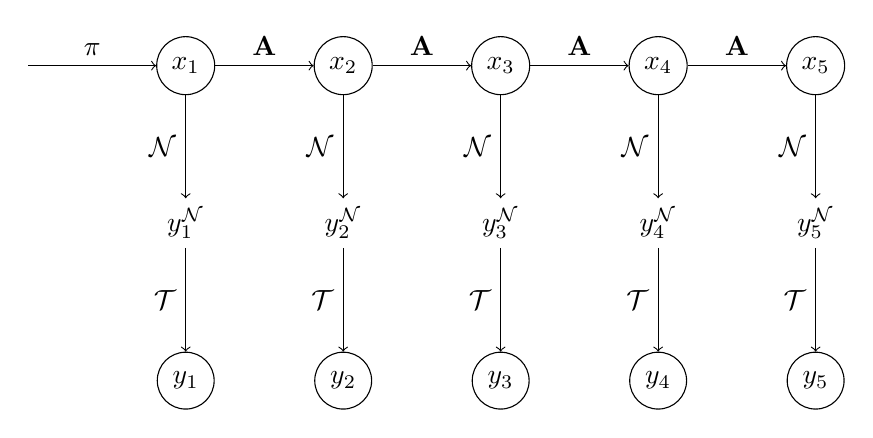
\begin{tikzpicture}[main/.style = {draw, circle}, node distance = 20mm and 10mm] 
        \node[main] (1) {$x_1$};
        \node[main] (2) [right of=1] {$x_2$};
        \node[main] (3) [right of=2] {$x_3$};
        \node[main] (4) [right of=3] {$x_4$};
        \node[main] (5) [right of=4] {$x_5$};


        \node[] (11) [below of=1] {$y_1^{\mathcal N}$};
        \node[] (12) [below of=2] {$y_2^{\mathcal N}$};
        \node[] (13) [below of=3] {$y_3^{\mathcal N}$};
        \node[] (14) [below of=4] {$y_4^{\mathcal N}$};
        \node[] (15) [below of=5] {$y_5^{\mathcal N}$};

        \node[main] (21) [below of=11] {$y_1$};
        \node[main] (22) [below of=12] {$y_2$};
        \node[main] (23) [below of=13] {$y_3$};
        \node[main] (24) [below of=14] {$y_4$};
        \node[main] (25) [below of=15] {$y_5$};

        \draw[->] (-2, 0) -- node[above] {$\pi$} (1);
        \draw[->] (1) -- node[above] {$\textbf{A}$} (2);
        \draw[->] (2) --  node[above] {$\textbf{A}$} (3);
        \draw[->] (3) -- node[above] {$\textbf{A}$} (4);
        \draw[->] (4) -- node[above] {$\textbf{A}$} (5);
        
        \draw[->] (1) -- node[left] {$\mathcal N$} (11);
        \draw[->] (2) -- node[left] {$\mathcal N$} (12);
        \draw[->] (3) -- node[left] {$\mathcal N$} (13);
        \draw[->] (4) -- node[left] {$\mathcal N$} (14);
        \draw[->] (5) -- node[left] {$\mathcal N$} (15);

        \draw[->] (11) -- node[left] {$\mathcal T$} (21);
        \draw[->] (12) -- node[left] {$\mathcal T$} (22);
        \draw[->] (13) -- node[left] {$\mathcal T$} (23);
        \draw[->] (14) -- node[left] {$\mathcal T$} (24);
        \draw[->] (15) -- node[left] {$\mathcal T$} (25);
        
    \end{tikzpicture}    
    \caption{Schema of Flow Hidden Markov Model (for $t \in \mathbb N _{\leq 5}$).}
    \label{fig:flow_model_schema}
\end{figure}

% \textbf{TODO: powtórzyć wszystkie algorytmy dla nowego modelu czy tylko krok M w Forward-Backward?}

All algorithms  described in Section \ref{sec:hmm_algs} are valid for FlowHMM after a small adaptation in the emission probabilities:

\begin{equation*}
    \mathbbm B_i (v) = f_{\mathcal N} (\mathcal T_i^{-1}(v)) \cdot \Big| \prod_{f=1}^F \det \big(J^{-1}_{\mathcal T_i^{(f)}}(v)\big) \Big|\text{.}
\end{equation*}

Please note, that calculating the conditional emission probabilities need calculating the determinant of the Jacobian of the transformation $\mathcal T$, what makes the iterative forward-backward algorithm quite time-consuming. Below, we will show, how the formulas of Forward-Backward algorithm  updated for FlowHMM. Updates for other algorithms are similarly. 

Let us start with the loss function: 
\begin{equation*}
    \begin{aligned}
        \ell^{\star}(\Tilde{\Theta}; y_{1:T})  = & \sum_{i=1}^N \mathbbm P_{\Theta}(X_{1}=i) \log \Tilde{\pi}_{i}  +\\ 
        & +  \sum_{t=1}^{T-1} \sum_{i=1}^N  \sum_{j=1}^N \mathbbm P_{\Theta}(X_{t}=i, X_{t+1}=j) \log  \Tilde{\textbf{A}}_{ij}  +\\ 
        & +  \sum_{t=1}^T \sum_{i=1}^N \mathbbm P_{\Theta}(X_{t}=i) \log \Bigg( f_{\mathcal N} (\mathcal T_i^{-1}(y_t)) \cdot \Big| \prod_{f=1}^F \det \big(J^{-1}_{\Tilde{\mathcal T}_i^{(f)}}(y_t)\big) \Big| \Bigg)
    \end{aligned}
\end{equation*}

and the recursive formulas for forward probability:

\begin{subequations}
    \begin{equation*}
        \alpha_1(i) = \pi_i \cdot f_{\mathcal N} (\mathcal T_i^{-1}(y_1)) \cdot \Big| \prod_{f=1}^F \det \big(J^{-1}_{\Tilde{\mathcal T}_i^{(f)}}(y_1)\big) \Big|\text{,}
    \end{equation*}
    \begin{equation*}
        \alpha_t(i) = \sum_{j=1}^n \alpha_{t-1}(j) \textbf{A}_{ji} \cdot  f_{\mathcal N} (\mathcal T_i^{-1}(y_t)) \cdot \Big| \prod_{f=1}^F \det \big(J^{-1}_{\mathcal T_i^{(f)}}(y_t)\big) \Big|\text{,}
    \end{equation*}
    \begin{equation*}
        \mathbb P(Y_{1:T} = y_{1:T}) = \sum_{i=1}^n \alpha_T(i)\text{,}
    \end{equation*}
\end{subequations}

and backward probability:

\begin{subequations}
    \begin{equation*}
        \beta_T(i) = 1\text{,}
    \end{equation*}
    \begin{equation*}
        \beta_t(i) = \sum_{j=1}^n \textbf{A}_{ij}  \cdot f_{\mathcal N} (\mathcal T_j^{-1}(y_t)) \cdot \Big| \prod_{f=1}^F \det \big(J^{-1}_{\Tilde{\mathcal T}_j^{(f)}}(y_t)\big) \Big| \cdot \beta_{t+1}(j)\text{,}
    \end{equation*}
    \begin{equation*}
        \mathbb P(Y_{1:T} = y_{1:T}) = \sum_{j=1}^N \pi_j  \cdot f_{\mathcal N} (\mathcal T_j^{-1}(y_1)) \cdot \Big| \prod_{f=1}^F \det \big(J^{-1}_{\Tilde{\mathcal T}_j^{(f)}}(y_1)\big) \Big|  \cdot \beta_1(j)\text{.}
    \end{equation*}
\end{subequations}



Now, we can calculate the probabilities from the step E:
$$\gamma_t^{(k)}(i) = \frac {\alpha_t^{(k)}(i) \beta_t^{(k)}(i)} {\sum_{j=1}^n \alpha_t^{(k)}(j) \beta_t^{(k)}(j)}\text{,}$$

$$\xi_t^{(k)}(i, j) = \frac{\alpha_{t}^{(k)}(i) \textbf{A}^{(k)}_{ij} \cdot  f_{\mathcal N} \big((\mathcal T^{(k)}_j)^{-1}(y_{t+1})\big) \cdot \Big| \prod_{f=1}^F \det \big(J^{-1}_{(\mathcal T^{(f)}_j)^{(k)}}(y_{t+1})\big) \Big|  \cdot \beta_{t+1}^{(k)}(j)}{\sum_{j=1}^n \alpha_t^{(k)}(j) \beta_{t}^{(k)}(j)}\text{.}$$

In the M step, the MC parameters updates as in Equations (\ref{eq:m_update_pi}, \ref{eq:m_update_a}). The update of the emission model is made via a number of steps in a gradient based learning procedure of the neural network. Such update may not lead to maximization of the emission model, but just an improvement (full maximization is not performed in each iteration due to the complexity of the emission model). 

\section{Co-occurrence-based learning for continuous models}

Let us start with a generalization of the co-occurrence matrix for continuous observations. 

\begin{definition}{Empirical continuous co-occurrence matrix}

The empirical co-occurrence matrix $\mathcal{Q}^{gt}$ for continuous observations summarises  the ratio of consecutive occurrences of each pair of discretized values: 

\begin{equation}\label{eq:c_cooc_gt}
    \mathcal{Q}^{gt}_{vw} = \frac {\#\{t: \mathcal D(y_t) =  v^{\mathcal D}, \mathcal D(y_{t+1}) = w ^{\mathcal D}\}} {T-1}\text{.}
\end{equation}
\end{definition}


\begin{definition}{Estimated continuous co-occurrence matrix}

The estimated co-occurrence matrix $\mathcal{Q}$ summarises  the probabilities of consecutive occurrences of each pair of discretized values: 

\begin{equation}\label{eq:c_cooc_mat}
    \mathcal{Q}_{vw} = \mathbbm P \big(\mathcal D(y_t) =  v^{\mathcal D}, \mathcal D(y_{t+1}) = w ^{\mathcal D}\big) \text{.}
\end{equation}
\end{definition}

We will approximate the probability of observing the discretized value as:

\begin{equation*}
\begin{aligned}
     \mathbbm P (\mathcal D (y) = v^{\mathcal D} | x = i) 
    & = \int_{\{y\in \mathbbm R^m: \mathcal D (y) = v^{\mathcal D} \}} 
    f_{\mathcal N} (\mathcal T_i^{-1}(y)) \cdot \Big| \prod_{f=1}^F \det \big(J^{-1}_{\mathcal T_i^{(f)}}(y)\big) \Big|
    dy
    \approx \\
    & \approx \frac{
    f_{\mathcal N} (\mathcal T_i^{-1}(\mathcal D (y))) \cdot \Big| \prod_{f=1}^F \det \big(J^{-1}_{\mathcal T_i^{(f)}}(\mathcal D (y))\big) \Big|
    }{
    \sum_{w^{\mathcal D} \in \mathcal{Y^{\mathcal D}}}
    f_{\mathcal N} (\mathcal T_i^{-1}(w^{\mathcal D})) \cdot \Big| \prod_{f=1}^F \det \big(J^{-1}_{\mathcal T_i^{(f)}}(w^{\mathcal D})\big) \Big|
    } =: \mathbbm B_i^{\mathcal D}(y)\text{.}
\end{aligned}
\end{equation*} 

We can also consider the discretized distribution as a matrix where $(\mathbbm B_i^{\mathcal D}(v^{\mathcal D}))_{v^{\mathcal D} \in \mathcal Y ^{\mathcal D}}$ is the $i$th row of the matrix $\mathbbm B^{\mathcal D}$. Using above formulas, we can calculate the co-occurrence matrix from the parameter similarly as in a discrete case:

\begin{equation}\label{eq:c_cooc_fact}
    \mathcal{Q} = (\mathbbm B ^{\mathcal D})^T \textbf{S} \mathbbm B^{\mathcal D}\text{.}
\end{equation}


\subsection{Example: continuous co-occurrence for GaussianHMM}

In this example, we will illustrate how to calculate the continuous co-occurrence matrices for GaussianHMM. We will continue the example \ref{sec:hmm_gaussian}, use the same model and the observed sequence (\ref{eq:ex_gaussian}).

First, we need to define the grid. We will use the quasi-random Sobol grid with $M^{\mathcal D} = 4$ values:

\begin{equation*}
% \begin{aligned}
    \mathcal Y ^{\mathcal D}_{QS} = \left\{ 
    \begin{array}{c}
        \left( \begin{array}{c}
        2.99\\1.94
        \end{array} \right),
        \left( \begin{array}{c}
        -0.72\\-1.04
        \end{array} \right),
        \left( \begin{array}{c}
        2.07\\2.75
        \end{array} \right),
        \left( \begin{array}{c}
        4.83\\-2.09
        \end{array} \right)
        \end{array} \right\}\text{.}
% \end{aligned}
\end{equation*}
Now we can discretize the observed secuence:
\begin{equation*}
\begin{aligned}
Y ^{\mathcal D} = &
\textcolor{teal}{\left( \begin{array}{c}4.83\\-2.09\end{array} \right)}
, \textcolor{purple}{\left( \begin{array}{c}2.99\\1.94\end{array} \right)}
, \textcolor{purple}{\left( \begin{array}{c}2.99\\1.94\end{array} \right)}
, \textcolor{blue}{\left( \begin{array}{c}-0.72\\-1.04\end{array} \right)}
, \textcolor{teal}{\left( \begin{array}{c}4.83\\-2.09\end{array} \right)}
, \textcolor{purple}{\left( \begin{array}{c}2.99\\1.94\end{array} \right)}
, \\
&  \textcolor{blue}{\left( \begin{array}{c}-0.72\\-1.04\end{array} \right)}
, \textcolor{teal}{\left( \begin{array}{c}4.83\\-2.09\end{array} \right)}
, \textcolor{purple}{\left( \begin{array}{c}2.99\\1.94\end{array} \right)}
, \textcolor{purple}{\left( \begin{array}{c}2.99\\1.94\end{array} \right)}
, \textcolor{purple}{\left( \begin{array}{c}2.99\\1.94\end{array} \right)}
, \textcolor{purple}{\left( \begin{array}{c}2.99\\1.94\end{array} \right)}
, \\
&  \textcolor{purple}{\left( \begin{array}{c}2.99\\1.94\end{array} \right)}
, \textcolor{blue}{\left( \begin{array}{c}-0.72\\-1.04\end{array} \right)}
, \textcolor{teal}{\left( \begin{array}{c}4.83\\-2.09\end{array} \right)}
, \textcolor{teal}{\left( \begin{array}{c}4.83\\-2.09\end{array} \right)}\text{.}
 \end{aligned}   
\end{equation*}
We can rewrite it using the indexes of the grid elements:
\begin{equation*}
\begin{aligned}
Y ^{\mathcal D} = &
    \textcolor{teal}{v^{\mathcal D}_4}
, \textcolor{purple}{v^{\mathcal D}_1}
, \textcolor{purple}{v^{\mathcal D}_1}
, \textcolor{blue}{v^{\mathcal D}_2}
, \textcolor{teal}{v^{\mathcal D}_4}
, \textcolor{purple}{v^{\mathcal D}_1}
, \textcolor{blue}{v^{\mathcal D}_2}
, \textcolor{teal}{v^{\mathcal D}_4}
, \\ &  \textcolor{purple}{v^{\mathcal D}_1}
, \textcolor{purple}{v^{\mathcal D}_1}
, \textcolor{purple}{v^{\mathcal D}_1}
, \textcolor{purple}{v^{\mathcal D}_1}
, \textcolor{purple}{v^{\mathcal D}_1}
, \textcolor{blue}{v^{\mathcal D}_2}
, \textcolor{teal}{v^{\mathcal D}_4}
, \textcolor{teal}{v^{\mathcal D}_4}\text{.}
\end{aligned}
\end{equation*}
The discretization of the data is also illustrated in Figure \ref{fig:cont_cooc}.

\begin{figure}[!ht]
    \centering
    \includegraphics[scale=0.54]{cont_cooc_example.eps}
    \includegraphics[scale=0.54]{cont_cooc_example_regions.eps}
    \caption{The above pictures illustrate the discretization procedure for 2D data. Crosses mark the grid elements, dots mark the observations, colors mark the discrete values, elipses showing the true distribution of the HMM emission. On the left Figure you can see discretized sequence, numbers mark the order of observations. On the right picture you can see the discretization rules (regions resulting in a discrete value), the numers mark the indexes of the nodes in grid.}
    \label{fig:cont_cooc}
\end{figure}
\pagebreak

Now we are able to calculate the continuous co-occurrence matrix derived from the data:
\begin{equation*}
    \mathcal Q^{gt} = \frac 1 {15}  
    \left[\begin{array}{rrrr}
         5 &  3 &  0 &  0 \\
         0 &  0 &  0 &  3 \\
         0 &  0 &  0 &  0 \\
         3 &  0 &  0 &  1 \\
\end{array} \right] 
\approx 
\left[\begin{array}{rrrr}
        0.333 & 0.200 & 0.000 & 0.000 \\
        0.000 & 0.000 & 0.000 & 0.200 \\
        0.000 & 0.000 & 0.000 & 0.000 \\
        0.200 & 0.000 & 0.000 & 0.067 \\
\end{array} \right] 
\end{equation*}


We would also like to derive the continuous co-occurrence matrix from the data. Please note, that the state co-occurrence matrix is the same as in example \ref{sec:cooc_example_disc} (see Equation (\ref{eq:s_example}). 
So we need to specify discretized emission matrix $\mathbbm B^{\mathcal D}$. First, let us calculate the emission density function for each hidden state at the points from grid:

\begin{equation*}
\begin{aligned}
    \mathbbm B(\mathcal Y^{\mathcal D}) & = \left[\begin{array}{cccc}
    \mathbbm B_1(v^{\mathcal D}_1) & \mathbbm B_1(v^{\mathcal D}_2) & \mathbbm B_1(v^{\mathcal D}_3) & \mathbbm B_1(v^{\mathcal D}_4) \\
    \mathbbm B_2(v^{\mathcal D}_1) & \mathbbm B_2(v^{\mathcal D}_2) & \mathbbm B_2(v^{\mathcal D}_3) & \mathbbm B_2(v^{\mathcal D}_4) \\
    \mathbbm B_3(v^{\mathcal D}_1) & \mathbbm B_3(v^{\mathcal D}_2) & \mathbbm B_3(v^{\mathcal D}_3) & \mathbbm B_3(v^{\mathcal D}_4) \\
    \end{array} \right] \\
    & \approx \left[\begin{array}{cccc}
    0.000001 & 0.038769 & 0.000001 & 0.000002 \\
    0.000000 & 0.000001 & 0.000000 & 0.000327 \\
    0.078506 & 0.000000 & 0.012336 & 0.000000 \\
    \end{array} \right].
\end{aligned}
\end{equation*}
Now, we need to normalize rows of the matrix:
\begin{equation*}
    \mathbbm B^{\mathcal D} = 
    \left[\begin{array}{cccc}
    0.000028 & 0.999901 & 0.000027 & 0.000044 \\
    0.000130 & 0.003088 & 0.000047 & 0.996735 \\
    0.864191 & 0.000005 & 0.135798 & 0.000005 \\
    \end{array} \right].
\end{equation*}
Using the Equation \ref{eq:c_cooc_mat} we obtain the continuous co-occurrence matrix:
\begin{equation*}
    \mathcal Q = \left[\begin{array}{cccc}
    0.038410 & 0.011110 & 0.006036 & 0.000002 \\
    0.000036 & 0.001468 & 0.000006 & 0.012840 \\
    0.006036 & 0.001746 & 0.000949 & 0.000001 \\
    0.011076 & 0.000027 & 0.001741 & 0.008516 \\
    \end{array} \right].
\end{equation*}



% When learning the model's parameters we will minimize the difference between the co-occurrence matrix obtained from the observed sequence $\mathcal Q ^{gt}$ and the co-occurrence matrix obtained from the parameters $\mathcal Q$. The matrix $\mathcal Q ^{gt}$ is calculated once and summarises the input sequence. The matrix  $\mathcal Q$ is calculated in each iteration of the algorithm and relies on the current parameter estimation. 

% \subsection{Co-occurrence Matrix $\mathcal Q ^{gt}$}

% The co-occurrence matrix for one training sequence can be stated as:

% \begin{equation} %\label{eq:omega_gt}
%     \textbf{Q}^{GT}_{ij} = \frac{\#\{t: Y_t \in r_i, Y_{t+1} \in r_j\}} {T-1} 
% \end{equation}

% For several training sequences (where the upper index is for the index of the sequence):

% \begin{equation}  %\label{eq:omega_gt}
%     \textbf{Q}^{GT}_{ij} = \frac{\sum_{i}\#\{t: Y_t^{(i)} \in r_i, Y_{t+1}^{(i)} \in r_j\}} {\sum_{i} [T^{(i)}-1]} 
% \end{equation}

% Calculating the co-occurrence matrix from data has linear time complexity concerning the length of the sequence and constant memory usage (depends squarely on the grid size). 

% \subsection{Co-occurrence Matrix $\mathcal Q$}

% We also calculate the co-occurrence matrix from the model parameters. It is possible with the assumption of stationarity of the Markov Chain $X$.

% As the set of observable values changes after discretizing the data, we need also to rewrite the emission probabilities. Now, it can be stated as a matrix:

% \begin{equation}
%     B^{\mathcal D}_{ij} = \frac{B_i(g_j)}{\sum_{t=1}^M B_i(g_t)} 
% \end{equation}



% When we assume, that the Markov Chain $X$ is stationary, we can present any transition probability as:

% \begin{equation} \label{eq:tehta0}
%     S_{t, l} = A_{tl}\pi_t
% \end{equation}

% The co-occurrence of two consecutive values means, that we first emmit a value $v_{i_1}$ from a state $s_{i_1}$, transit to a state $s_{i_2}$ and emit $v_{i_2}$ for any combination of hidden states  $s_{i_1}$,  $s_{i_2}$:

% \begin{equation} \label{eq:omega0}
%     \textbf{Q} =( B^{\mathcal D})^T S B^{\mathcal D}
% \end{equation}

% Using the original model parameters we can express the $(i, j)$th element of the matrix as:

% \begin{equation} \label{eq:omega}
%     \textbf{Q}_{i,  j}  = \sum_{t=1}^n \sum_{l=1}^n \pi_t B^{\mathcal D}_{iv} A_{t,  l} B^{\mathcal D}_{l, j}
% \end{equation}

% In the implementation, we will use an uncontrined matrix $\Tilde{S}$, such that: 

% \begin{equation}
%     S_{ij} = \frac{exp(\Tilde{S}_{ij})}{\sum_{t=1}^N exp(\Tilde{S}_{iv})}
% \end{equation}

% The above transformation is called soft-max.


% The loss function in this case is the Kulback-Leibler distance between the co-occurrence matrices:

% \begin{equation}
%     A, B, \pi = \argmin_{A, B, \pi} KL(\textbf{Q}^{gt}, \textbf{Q})
% \end{equation}

% To find this minimum we will use a gradient-based, numerical optimization procedure such as Stochastic Gradient Descent or Adam.

\section{Example: FlowHMM training}

In this example, we show the emission distributions learning process: we plot the distributions obtained from FlowHMM afetr each 10 iterations. Please see Figure \ref{fig:flow_traning} to follow the FlowHMM training process. 

\begin{figure}
    \centering
    \begin{subfigure}{0.32\textwidth}
    \includegraphics[scale=0.35]{flow_on_moons_0_penalty=0_grid.png}
    \caption{ 1 iteration.}
    \end{subfigure}
    \begin{subfigure}{0.32\textwidth}
    \includegraphics[scale=0.35]{flow_on_moons_1_penalty=0_grid.png}
    \caption{ 11 iterations.}
    \end{subfigure}
    \begin{subfigure}{0.32\textwidth}
    \includegraphics[scale=0.35]{flow_on_moons_2_penalty=0_grid.png}
    \caption{ 21 iterations.}
    \end{subfigure}
    
    \begin{subfigure}{0.32\textwidth}
    \includegraphics[scale=0.35]{flow_on_moons_3_penalty=0_grid.png}
    \caption{ 31 iterations.}
    \end{subfigure}
    \begin{subfigure}{0.32\textwidth}
    \includegraphics[scale=0.35]{flow_on_moons_4_penalty=0_grid.png}
    \caption{ 41 iterations.}
    \end{subfigure}
    \begin{subfigure}{0.32\textwidth}
    \includegraphics[scale=0.35]{flow_on_moons_5_penalty=0_grid.png}
    \caption{ 51 iterations.}
    \end{subfigure}

    \begin{subfigure}{0.32\textwidth}
    \includegraphics[scale=0.35]{flow_on_moons_6_penalty=0_grid.png}
    \caption{ 61 iterations.}
    \end{subfigure}
    \begin{subfigure}{0.32\textwidth}
    \includegraphics[scale=0.35]{flow_on_moons_7_penalty=0_grid.png}
    \caption{ 71 iterations.}
    \end{subfigure}
    \begin{subfigure}{0.32\textwidth}
    \includegraphics[scale=0.35]{flow_on_moons_8_penalty=0_grid.png}
    \caption{ 81 iterations.}
    \end{subfigure}
    
    \begin{subfigure}{0.32\textwidth}
    \includegraphics[scale=0.35]{flow_on_moons_9_penalty=0_grid.png}
    \caption{ 91 iterations.}
    \end{subfigure}
    \begin{subfigure}{0.32\textwidth}
    \includegraphics[scale=0.35]{flow_on_moons_10_penalty=0_grid.png}
    \caption{ 101 iterations.}
    \end{subfigure}
    \begin{subfigure}{0.32\textwidth}
    \includegraphics[scale=0.35]{flow_on_moons_11_penalty=0_grid.png}
    \caption{ 111 iterations.}
    \end{subfigure}


    \caption{FlowHMM emission after several model training iterations.}
    \label{fig:flow_traning}
\end{figure}

\chapter{Experiments} \label{sec:experiments}

The aim of the experiments conducted was to study the properties of the components added to the original model. 

% The first  experiments concern the discretization. We perform numerical experiments to test if the disretization preserves the original distribution. Then, we compare the co-occurrence matrix from the data and the model the data was generated from. In the second experiment, we study the co-occurrence-based learning algorithm on how good results we can obtain. In the following step we look on how well the selected normalizing flow architecture can capture the complicated multidimensional distributions. In the final experiment we look on the whole model with co-occurrence-based learning algorithm and it results in a high dimensional case.

\section{Experiment 0: GaussianHMM + Co-occurrence + true initialization}

In the zero experiment, we check if using the co-occurrence learning schema ifluences the results of the model massivly. As the co-occurrence based schema has been recently used by several scientist, it is mostly a sanity check for our implementation and a way to get familiar with the model in practice. 

First, we sample training sequence of the length $T$ and testing sequence of length $T / 10$. Then we train a standard model 20 times (random initialization of kmeans used to initialize emission parameters could influence model results) and evaluate it on testing data. 
% We calculate the following metrics:
% \begin{itemize}
%     \item model score
%     \item state prediction accuracy
% \end{itemize}
Then, for each discretization technique we train a custom model (after initializing with true model parameters) and evaluate it, 20 times for each.

We used one data sample (quite big for this problem) for the whole experiment and studied, how the randomness of the discretization and initialization affects the results. 

\subsection{Setup} \label{sec:ex0_setup}

\begin{itemize}
    \item $T = 10000$ - training sequence length
    \item $N = 3$ - number of hidden states (model hyperparameter)
    \item number of repetitions for each model: 20
    \item discretization techniques:
    \begin{itemize}
        \item $OG$ -- ordinary grid 
        \item $RO$ -- random observation grid 
        \item $RU$ -- random uniform ($\mathcal U (\hat{\mathcal Y})$) grid 
        \item $LH$ -- latin hypercube sampled grid 
        \item $LH_q$ -- latin hypercube quantile sampled grid 
        \item $QS$ -- quasi-random Sobol grid 
        \item $QH$ -- quasi-random Halton grid 
    \end{itemize}
    \item evaluation metrics:
    \begin{itemize}
        \item model score (loglikelihood)
        \item state prediction accuracy
        \item KL divergence between $Q$ and $Q^{gt}$ (calculated only for custom models)
        \item total variation distance ($d_{TV}$) between $Q$ and $Q^{gt}$ (calculated only for custom models)
    \end{itemize}
    \item true model parameters:
    \begin{itemize}
        \item $\pi = \left(\begin{array}{ccc} 0.6 & 0.3 & 0.1 \end{array}\right)$ 
        \item $\textbf{A} = \left(\begin{array}{ccc} 0.7 & 0.2 & 0.1 \\ 0.3 & 0.5 & 0.2 \\ 0.3 & 0.3 & 0.4 \end{array}\right)$ 
        \item $(\mu_1, \mu_2, \mu_3) = \left(\begin{array}{ccc}\left(\begin{array}{c} 0 \\ 0 \end{array}\right) & \left(\begin{array}{c} 3 \\ -3 \end{array}\right) & \left(\begin{array}{c} 4 \\ 3 \end{array}\right)\end{array}\right)$ 
        \item $(\Sigma_1, \Sigma_2, \Sigma_3) = \left(\begin{array}{ccc}\left(\begin{array}{cc} 0.8 & -0.4 \\ -0.4 & 0,96 \end{array}\right) & \left(\begin{array}{cc} 0.48 & -0.4 \\ -0.4 & 0.96 \end{array}\right) & \left(\begin{array}{cc} 1.2 & 0.4 \\ 0.4 & 1.76 \end{array}\right)\end{array}\right)$ 
    \end{itemize}
    Please note that the starting distribution does not follow the assumption of stationarity. However, as we sample one long sequence it does not really matter. 
    \item hyperparameter settings (used in gread search):
    \begin{itemize}
        \item learning rate: $0.001$, $0.01$, $0.03$, $0.1$
        \item number of iterations: $1000$
        \item number of discrete values $M^{\mathcal D}$: $2^2$, $2^4$, $2^6$
    \end{itemize}
    \item optimizer: SGD
\end{itemize}

\subsection{Goal} 

Our goal is to see the influence of the discretization on the model (if it disturbs the results), check the co-occurrence based learning schema and a sanity check for our custom implementation. 

\subsection{Results}

\begin{figure}[!ht]
    \centering
    \includegraphics[scale=0.085]{W&B Chart 8_11_2023, 10 15 01 AM.png}
    \includegraphics[scale=0.085]{W&B Chart 8_11_2023, 10 15 33 AM.png}
    \caption{Training logs (logging each 100 iterations, metrics calculated on the training data) in zero experiment for selected runs with Halton discretization. $M^{\mathcal D} = 16$, 1000 iterations and learning rates 0.001, 0.01, 0.03, 0.1.}
    \label{fig:training0}
\end{figure}

Let us first look at the learning process\footnote{visualizations from \href{https://wandb.ai/}{https://wandb.ai/}.} illustrated at Figure \ref{fig:training0}. We can see that most of the discrease of the objective (KL for Q matrix) is done in the first 100 iterations. Bigger learning rates lead to overfitting, which results in bigger decrease of the likelihood (please note that due to the initialization the model is converged to true parameters at the beginning of the training).

Now, let us take a closer look at those two metrics for all runs at Figure \ref{fig:res0} performed on test data. We can observe that for increasing $M^{\mathcal D}$, the KL divergence grows massivly, espessialy for random observations. We consider that it might be caused by distinguishing between very close value, especially visible for a shorter test sequence (look at Figure \ref{fig:0_og_nodes_4}, left plot).


\begin{figure}[!ht]
    \centering
    \includegraphics[scale=0.4]{0_kl_1000__4_on_lr.eps}
    \includegraphics[scale=0.4]{0_ll_1000__4_on_lr.eps}
    
    \includegraphics[scale=0.4]{0_kl_1000__16_on_lr.eps}
    \includegraphics[scale=0.4]{0_ll_1000__16_on_lr.eps}
    
    \includegraphics[scale=0.4]{0_kl_1000__64_on_lr.eps}
    \includegraphics[scale=0.4]{0_ll_1000__64_on_lr.eps}
    \caption{KL divergence and log-likelihood for incressing learning rate. }
    \label{fig:res0}
\end{figure}
 
 The second surprising thing is the massive drop of log-likelihood for ordinary grid of size 4. It becomes more clear, if we look at Figure \ref{fig:0_og_nodes_4}, right plot. The nodes do not follow the structure of continuous probability distribution at all, thus the parameter estimation might be distinctly biased. Please note, that quasi random numbers do not perform badly in any of presented settings (they might not give stunning results, but seem to be reliable for such tasks). 
 
\begin{figure}[!ht]
    \centering
    \includegraphics[scale=0.45]{0_nodes_random_64.eps}
    \includegraphics[scale=0.45]{0_nodes_grid_4.eps}
    \caption{True distribution and used discrete values.}
    \label{fig:0_og_nodes_4}
\end{figure}


Please see the detailed results in the following Tables \ref{tab:res_0_4}, \ref{tab:res_0_16}, \ref{tab:res_0_64},  with marked \colorbox{orange}{the worst} and \colorbox{green}{the best} results for each $M^{\mathcal D}$.

\pagebreak 

\begin{table}[!ht]
\centering
\caption{Results for $M^{\mathcal D}=4$.}
\vspace{5mm}
\begin{tabular}{llllll}  \hline
& lr &   KL &                      ll &               acc &              $d_{TV}$ \\ \hline
$OG$ & 0.001 &     0.030 $\pm$ 0.000 &       -3553.95 $\pm$ 0.000 &    \colorbox{green}{0.983 $\pm$ 0.000} &     0.020 $\pm$ 0.000 \\
        & 0.010 &     0.010 $\pm$ 0.000 &      -3688.017 $\pm$ 0.000 &    0.981 $\pm$ 0.000 &    0.011 $\pm$ 0.000 \\
        & 0.030 &    0.001 $\pm$ 0.000 &      -4042.552 $\pm$ 0.000 &    0.976 $\pm$ 0.000 &    0.004 $\pm$ 0.000 \\
        & 0.100 &    \colorbox{green}{0.001 $\pm$ 0.000} &      \colorbox{orange}{-4601.578 $\pm$ 0.000} &     0.970 $\pm$ 0.000 &    \colorbox{green}{0.002 $\pm$ 0.000} \\
$QH$ & 0.001 &   0.29 $\pm$ 0.234 &    \colorbox{green}{-3551.370 $\pm$ 44.064} &  0.981 $\pm$ 0.001 &  0.057 $\pm$ 0.027 \\
        & 0.010 &  0.326 $\pm$ 0.481 &   -3573.687 $\pm$ 52.106 &  0.981 $\pm$ 0.003 &  0.051 $\pm$ 0.042 \\
        & 0.030 &  0.246 $\pm$ 0.196 &   -3590.759 $\pm$ 64.375 &  0.981 $\pm$ 0.002 &   0.050 $\pm$ 0.026 \\
        & 0.100 &    0.378 $\pm$ 0.500 &  -3757.705 $\pm$ 436.503 &  0.959 $\pm$ 0.089 &   0.055 $\pm$ 0.040 \\
$LH_q$ & 0.001 &    0.261 $\pm$ 0.2 &    -3557.250 $\pm$ 45.375 &  0.981 $\pm$ 0.001 &  0.054 $\pm$ 0.024 \\
        & 0.010 &  0.283 $\pm$ 0.289 &   -3573.837 $\pm$ 41.476 &  0.982 $\pm$ 0.001 &  0.054 $\pm$ 0.029 \\
        & 0.030 &  0.276 $\pm$ 0.263 &   -3578.226 $\pm$ 36.846 &  0.981 $\pm$ 0.002 &  0.052 $\pm$ 0.029 \\
        & 0.100 &  0.216 $\pm$ 0.212 &   -3627.401 $\pm$ 92.971 &   0.980 $\pm$ 0.006 &  0.048 $\pm$ 0.025 \\
$LH$ & 0.001 &  0.353 $\pm$ 0.449 &   -3553.964 $\pm$ 44.465 &  0.981 $\pm$ 0.003 &  0.055 $\pm$ 0.039 \\
        & 0.010 &    0.3 $\pm$ 0.332 &   -3589.148 $\pm$ 53.799 &  0.982 $\pm$ 0.002 &  0.053 $\pm$ 0.032 \\
        & 0.030 &  0.235 $\pm$ 0.252 &   -3612.650 $\pm$ 119.956 &  0.979 $\pm$ 0.006 &   0.045 $\pm$ 0.030 \\
        & 0.100 &   0.379 $\pm$ 0.360 &  -3787.877 $\pm$ 503.387 &   0.974 $\pm$ 0.020 &  0.059 $\pm$ 0.038 \\
$RO$ & 0.001 &  0.135 $\pm$ 0.125 &   -3542.749 $\pm$ 39.061 &  0.982 $\pm$ 0.003 &   0.039 $\pm$ 0.002 \\
        & 0.010 &   0.198 $\pm$ 0.210 &  -3637.569 $\pm$ 244.821 &  0.976 $\pm$ 0.019 &  0.048 $\pm$ 0.029 \\
        & 0.030 &   0.285 $\pm$ 0.320 &   -3768.150 $\pm$ 482.564 &  0.952 $\pm$ 0.091 &  0.053 $\pm$ 0.037 \\
        & 0.100 &  0.124 $\pm$ 0.176 &  -3697.383 $\pm$ 378.598 &   0.963 $\pm$ 0.070 &  0.033 $\pm$ 0.023 \\
$QS$ & 0.001 &  0.354 $\pm$ 0.415 &   -3575.492 $\pm$ 55.954 &  0.981 $\pm$ 0.001 &   0.061 $\pm$ 0.040 \\
        & 0.010 &  0.533 $\pm$ 0.996 &   -3602.981 $\pm$ 86.557 &  0.981 $\pm$ 0.002 &  0.058 $\pm$ 0.043 \\
        & 0.030 &   0.27 $\pm$ 0.202 &      -3607.220 $\pm$ 71.300 &  0.981 $\pm$ 0.002 &  0.052 $\pm$ 0.028 \\
        & 0.100 &  0.335 $\pm$ 0.455 &  -3710.839 $\pm$ 286.698 &   \colorbox{orange}{0.970 $\pm$ 0.035} &  0.056 $\pm$ 0.032 \\
$RU$ & 0.001 &  \colorbox{orange}{0.548 $\pm$ 0.452} &    -3552.826 $\pm$ 55.130 &  0.982 $\pm$ 0.002 &  \colorbox{orange}{0.074 $\pm$ 0.042} \\
        & 0.010 &  0.374 $\pm$ 0.344 &    -3570.173 $\pm$ 33.770 &  0.981 $\pm$ 0.002 &  0.063 $\pm$ 0.039 \\
        & 0.030 &  0.518 $\pm$ 0.448 &  -3688.467 $\pm$ 170.648 &  0.974 $\pm$ 0.015 &   0.074 $\pm$ 0.040 \\
        & 0.100 &  0.407 $\pm$ 0.401 &  -3827.894 $\pm$ 450.446 &  0.973 $\pm$ 0.021 &  0.062 $\pm$ 0.038 \\ \hline
\end{tabular}
\label{tab:res_0_4}
\end{table}

\pagebreak 

\begin{table}[!ht]
\centering
\caption{Results for $M^{\mathcal D}=16$.}
\vspace{5mm}
\begin{tabular}{llllll}  \hline
& lr &   KL &                      ll &               acc &              $d_{TV}$ \\ \hline
$OG$ & 0.001 &    0.059 $\pm$ 0.000 &      -3622.845 $\pm$ 0.000 &    0.982 $\pm$ 0.000 &    0.006 $\pm$ 0.000 \\
        & 0.010 &    0.029 $\pm$ 0.000 &      -3659.083 $\pm$ 0.000 &    0.982 $\pm$ 0.000 &    0.003 $\pm$ 0.000 \\
        & 0.030 &    \colorbox{green}{0.024 $\pm$ 0.000} &      -3681.153 $\pm$ 0.000 &    \colorbox{green}{0.983 $\pm$ 0.000} &    0.002 $\pm$ 0.000 \\
        & 0.100 &    0.035 $\pm$ 0.000 &      -3710.129 $\pm$ 0.000 &    0.983 $\pm$ 0.000 &    \colorbox{green}{0.001 $\pm$ 0.000} \\
$QH$ & 0.001 &  0.371 $\pm$ 0.162 &    -3586.05 $\pm$ 36.735 &  0.981 $\pm$ 0.002 &  0.015 $\pm$ 0.004 \\
        & 0.010 &  0.302 $\pm$ 0.162 &   -3635.497 $\pm$ 32.692 &   0.980 $\pm$ 0.002 &  0.013 $\pm$ 0.004 \\
        & 0.030 &   0.496 $\pm$ 0.510 &   -3652.996 $\pm$ 65.255 &  0.979 $\pm$ 0.003 &  0.015 $\pm$ 0.005 \\
        & 0.100 &  0.434 $\pm$ 0.248 &   -3678.974 $\pm$ 52.867 &  0.978 $\pm$ 0.005 &  0.015 $\pm$ 0.005 \\
$LH_q$ & 0.001 &   0.328 $\pm$ 0.110 &   -3560.725 $\pm$ 19.309 &  0.981 $\pm$ 0.001 &  0.014 $\pm$ 0.002 \\
        & 0.010 &   0.510 $\pm$ 0.384 &   -3644.204 $\pm$ 81.043 &  0.977 $\pm$ 0.005 &  0.016 $\pm$ 0.005 \\
        & 0.030 &   0.424 $\pm$ 0.39 &   -3678.192 $\pm$ 87.409 &  0.977 $\pm$ 0.007 &  0.015 $\pm$ 0.005 \\
        & 0.100 &  0.504 $\pm$ 0.259 &  -3768.616 $\pm$ 206.296 &    0.970 $\pm$ 0.010 &  0.017 $\pm$ 0.003 \\
$LH$ & 0.001 &  0.364 $\pm$ 0.111 &   -3585.798 $\pm$ 27.782 &  0.981 $\pm$ 0.002 &  0.015 $\pm$ 0.003 \\
        & 0.010 &  0.461 $\pm$ 0.359 &   -3641.722 $\pm$ 55.312 &   0.980 $\pm$ 0.003 &  0.015 $\pm$ 0.005 \\
        & 0.030 &  0.596 $\pm$ 0.324 &   -3643.604 $\pm$ 43.653 &  0.977 $\pm$ 0.005 &  0.018 $\pm$ 0.005 \\
        & 0.100 &  0.651 $\pm$ 0.392 &   -3670.398 $\pm$ 71.306 &  0.976 $\pm$ 0.005 &  0.019 $\pm$ 0.006 \\
$RO$ & 0.001 &  0.453 $\pm$ 0.193 &   \colorbox{green}{-3549.581 $\pm$ 17.965} &  0.981 $\pm$ 0.002 &  0.018 $\pm$ 0.003 \\
        & 0.010 &  0.502 $\pm$ 0.237 &   -3669.289 $\pm$ 55.681 &  0.974 $\pm$ 0.006 &  0.019 $\pm$ 0.004 \\
        & 0.030 &  0.551 $\pm$ 0.372 &  -3738.688 $\pm$ 125.629 &   \colorbox{orange}{0.971 $\pm$ 0.010} &  0.018 $\pm$ 0.004 \\
        & 0.100 &  0.459 $\pm$ 0.216 &  \colorbox{orange}{-3816.443 $\pm$ 146.403} &  0.963 $\pm$ 0.014 &  0.018 $\pm$ 0.004 \\
$QS$ & 0.001 &  0.423 $\pm$ 0.317 &    -3590.592 $\pm$ 36.720 &  0.981 $\pm$ 0.002 &  0.017 $\pm$ 0.006 \\
        & 0.010 &   0.289 $\pm$ 0.170 &   -3628.127 $\pm$ 43.947 &   0.98 $\pm$ 0.002 &  0.012 $\pm$ 0.003 \\
        & 0.030 &  0.367 $\pm$ 0.261 &   -3643.792 $\pm$ 38.366 &  0.979 $\pm$ 0.003 &  0.013 $\pm$ 0.005 \\
        & 0.100 &  0.416 $\pm$ 0.202 &   -3679.885 $\pm$ 59.071 &  0.978 $\pm$ 0.006 &  0.015 $\pm$ 0.005 \\
$RU$ & 0.001 &  0.753 $\pm$ 0.509 &   -3592.362 $\pm$ 34.981 &   0.980 $\pm$ 0.002 &  0.017 $\pm$ 0.006 \\
        & 0.010 &  0.965 $\pm$ 1.256 &   -3650.533 $\pm$ 72.369 &  0.978 $\pm$ 0.005 &  0.019 $\pm$ 0.009 \\
        & 0.030 &  0.722 $\pm$ 0.507 &  -3718.258 $\pm$ 123.113 &   0.975 $\pm$ 0.010 &  0.019 $\pm$ 0.005 \\
        & 0.100 &  \colorbox{orange}{1.107 $\pm$ 1.087} &   -3773.460 $\pm$ 121.292 &  0.972 $\pm$ 0.015 &  \colorbox{orange}{0.021 $\pm$ 0.009} \\
\hline
\end{tabular}
\label{tab:res_0_16}
\end{table}

\pagebreak 

\begin{table}[!ht]
\centering
\caption{Results for $M^{\mathcal D}=64$.}
\vspace{5mm}
\begin{tabular}{llllll}  \hline
$OG$ & 0.001 &    \colorbox{green}{0.317 $\pm$ 0.000} &      -3546.121 $\pm$ 0.000 &    0.981 $\pm$ 0.000 &    0.002 $\pm$ 0.000 \\
        & 0.010 &    0.377 $\pm$ 0.000 &      -3557.596 $\pm$ 0.000 &    \colorbox{green}{0.982 $\pm$ 0.000} &    \colorbox{green}{0.001 $\pm$ 0.000} \\
        & 0.030 &     0.39 $\pm$ 0.000 &      -3556.214 $\pm$ 0.000 &    \colorbox{green}{0.982 $\pm$ 0.000} &    \colorbox{green}{0.001 $\pm$ 0.000} \\
        & 0.100 &    0.396 $\pm$ 0.000 &      -3554.542 $\pm$ 0.000 &    \colorbox{green}{0.982 $\pm$ 0.000} &    \colorbox{green}{0.001 $\pm$ 0.000} \\
$QH$ & 0.001 &  0.795 $\pm$ 0.241 &    \colorbox{green}{-3539.986 $\pm$ 9.109} &  0.981 $\pm$ 0.002 &    0.004 $\pm$ 0.000 \\
        & 0.010 &  0.918 $\pm$ 0.236 &   -3564.649 $\pm$ 18.697 &  0.979 $\pm$ 0.004 &  0.004 $\pm$ 0.001 \\
        & 0.030 &  0.958 $\pm$ 0.296 &   -3570.497 $\pm$ 26.242 &  0.978 $\pm$ 0.007 &  0.004 $\pm$ 0.001 \\
        & 0.100 &   0.929 $\pm$ 0.23 &   -3563.732 $\pm$ 19.934 &  0.978 $\pm$ 0.005 &    0.003 $\pm$ 0.000 \\
$LH_q$ & 0.001 &  2.319 $\pm$ 0.213 &   -3546.601 $\pm$ 10.369 &  0.981 $\pm$ 0.001 &    0.005 $\pm$ 0.000 \\
        & 0.010 &  2.192 $\pm$ 0.649 &   -3617.224 $\pm$ 22.802 &  0.977 $\pm$ 0.006 &  0.005 $\pm$ 0.001 \\
        & 0.030 &  1.964 $\pm$ 0.456 &   -3686.921 $\pm$ 65.993 &  0.975 $\pm$ 0.005 &    0.005 $\pm$ 0.000 \\
        & 0.100 &  2.174 $\pm$ 0.508 &   -3738.574 $\pm$ 103.38 &  0.968 $\pm$ 0.008 &    0.005 $\pm$ 0.000 \\
$LH$ & 0.001 &  1.033 $\pm$ 0.252 &   -3553.163 $\pm$ 14.974 &  0.981 $\pm$ 0.002 &  0.005 $\pm$ 0.001 \\
        & 0.010 &   1.18 $\pm$ 0.333 &   -3607.535 $\pm$ 58.396 &  0.977 $\pm$ 0.005 &  0.005 $\pm$ 0.001 \\
        & 0.030 &  1.381 $\pm$ 0.625 &   -3632.756 $\pm$ 46.405 &  0.973 $\pm$ 0.008 &  0.005 $\pm$ 0.001 \\
        & 0.100 &  1.726 $\pm$ 0.817 &   -3631.703 $\pm$ 73.778 &   0.974 $\pm$ 0.01 &  0.005 $\pm$ 0.001 \\
$RO$ & 0.001 &  3.811 $\pm$ 0.602 &    -3548.855 $\pm$ 12.16 &  0.981 $\pm$ 0.001 &    0.006 $\pm$ 0.000 \\
        & 0.010 &  4.013 $\pm$ 0.517 &    -3750.191 $\pm$ 50.32 &  0.975 $\pm$ 0.005 &    0.006 $\pm$ 0.000 \\
        & 0.030 &   \colorbox{orange}{4.320 $\pm$ 0.537} &   -3814.862 $\pm$ 73.221 &   0.966 $\pm$ 0.010 &  0.006 $\pm$ 0.001 \\
        & 0.100 &    4.28 $\pm$ 0.47 &   \colorbox{orange}{-3906.86 $\pm$ 148.125} &  \colorbox{orange}{0.950 $\pm$ 0.025} &    0.006 $\pm$ 0.000 \\
$QS$ & 0.001 &  0.659 $\pm$ 0.188 &     -3539.21 $\pm$ 10.77 &  0.981 $\pm$ 0.002 &  0.003 $\pm$ 0.001 \\
        & 0.010 &  0.838 $\pm$ 0.181 &   -3557.747 $\pm$ 13.716 &   0.98 $\pm$ 0.003 &  0.004 $\pm$ 0.001 \\
        & 0.030 &  0.898 $\pm$ 0.219 &   -3573.306 $\pm$ 24.863 &   0.973 $\pm$ 0.01 &  0.004 $\pm$ 0.001 \\
        & 0.100 &  0.845 $\pm$ 0.165 &   -3560.135 $\pm$ 24.537 &   0.975 $\pm$ 0.01 &  0.004 $\pm$ 0.001 \\
$RU$ & 0.001 &    1.222 $\pm$ 0.4 &   -3566.299 $\pm$ 27.853 &   0.98 $\pm$ 0.002 &  0.005 $\pm$ 0.001 \\
        & 0.010 &  1.603 $\pm$ 0.499 &   -3665.802 $\pm$ 86.981 &  0.973 $\pm$ 0.007 &  0.006 $\pm$ 0.001 \\
        & 0.030 &  1.761 $\pm$ 0.864 &  -3720.247 $\pm$ 130.673 &  0.968 $\pm$ 0.018 &  \colorbox{orange}{0.006 $\pm$ 0.002} \\
        & 0.100 &  1.968 $\pm$ 0.592 &  -3685.783 $\pm$ 100.317 &  0.974 $\pm$ 0.009 &  {0.006 $\pm$ 0.001} \\
\hline
\end{tabular}
\label{tab:res_0_64}
\end{table}

\newpage

\subsection{Conclusions}
\begin{itemize}
    \item Letting the model overfit leads to the decrease of log-likelihood. Generally, optimizing the KL divergence for the region-based co-occurrence matrices is not equivalent to optimizing log-likelihood. Training the model on discretized data may lead to biased parameter estimators.  
    \item As the experiment was more a sanity check than a real task for the model, the results are satisfying for all parameter settings. 
    \item The discretization techniques based on the data need the model to be tuned carefully. 
    \item Quasi random numbers perform most stable. 
    \item The model seems to work fine. 
\end{itemize}



\section{Experiment 1.1: GaussianHMM + Co-occurrence} \label{sec:ex11}



In the first experiment we compare the results of standard implementation of GaussianHMM with EM learning schema from hmmlearn library with how our custom implementation with co-occurrence based learning schema disturbs the true model. In this experiment, we train the model with custom representation from scratch, we initialize model parameters in the standard way (k-means like in the hmmlearn implementation: \linebreak\href{https://github.com/hmmlearn/hmmlearn/blob/main/lib/hmmlearn/hmm.py#L295}{https://github.com/hmmlearn/hmmlearn/blob/main/lib/hmmlearn/hmm.py\#L295}). 

\subsection{Setup} \label{sec:ex1_setup}

The setup was mostly transferred from the zero experiment (please see Section \ref{sec:ex0_setup}). Below we list only the elements which have changed.

\begin{itemize}
    \item hyperparameter settings (used in gread search):
    \begin{itemize}
        \item learning rate: $0.01$, $0.03$, $0.1$, $0.3$
        \item number of iterations: $2000$
    \end{itemize}
    \item optimizer: Adam
    \item learning rate scheduler: exponential, gamma = 0.9, use each 100 iterations
\end{itemize}

We changed the optimizer hyper-parameters settings, as we clearly need more time to learn. Also, the smallest learning rate was way to small for this task, as you can see in Figure \ref{fig:train_prel}.

% \begin{figure}[!ht]
%     \centering
%     \includegraphics[scale=0.15]{W&B Chart 8_11_2023, 9 04 30 lr 0.001.png}
%     \caption{Training (logging by 100 iterations) for lr=0.001, 2000 iterations, ordinary grid with 4 poitns.}
%     \label{fig:train_0.001}
% \end{figure}

\begin{figure}[!ht]
    \centering
    \includegraphics[scale=0.085]{W&B Chart 8_14_2023, 2 47 03 PM.png}
    \includegraphics[scale=0.085]{W&B Chart 8_14_2023, 2 46 49 PM.png}
    \caption{Training (logging by 100 iterations) for 2000 iterations, ordinary grid with 16 points.}
    \label{fig:train_prel}
\end{figure}

After running the experiment with 5000 iterations, we also decided to change the optimizer itself from SGD to Adam\footnote{\href{https://pytorch.org/docs/stable/generated/torch.optim.Adam.html}{https://pytorch.org/docs/stable/generated/torch.optim.Adam.html}} \cite{adam}. Even after decreasing the number of iterations to $2000$, the results obtained were were more stable (than those obtained with SGD).

\subsection{Goal}

In this experiment, we want to find out:

\begin{itemize}
    \item are the results obtained from our implementation are at least comparable with the results of the standard method?
    \item how stable are the results?
    \item can we expect good state prediction accuracy in an unsupervised setting?
    \item what discretization techniques work best?
\end{itemize}

\subsection{Results}

As the results have high variability, we decided to present the numerical results as ranges of obtained results instead of mean $\pm$ standard deviation in Tables \ref{tab:res_ex1_4}, \ref{tab:res_ex1_16}, \ref{tab:res_ex1_64} and visualize them as boxplots in Figures \ref{fig:res_ex1_4}, \ref{fig:res_ex1_16}, \ref{fig:res_ex1_64}. 

First, what we can observe is that the choice of learning rate makes a significant difference (see differences between the colored boxes in each group). Secondly, the ordinary grid discretization helps us to learn the co-occurrence matrix well. The quasi-random discretizations and the ordinary grid, give quite good results for all $M^{\mathcal D}$s. 

Let us also take a look at the relationship between two metrics (not optimized during the training schema) at Figure \ref{fig:cor_ex1}. We can see that there exists the correlations between the log-likelihood and the state prediction accuracy (it is about 0.3-0.6, detailed results are included in the plot titles).

\subsection{Conclusions}

\begin{itemize}
    \item Even though, the experiment was repeated with improvement of the results stability, they still vary between runs. There are multiple reasons for it: the randomness between the nodes selection, the randomness of model initialization, the hyper-parameters settings. 
    \item Results as in standard model are possible to obtain (however we need to select a model from multiple instances, which is not a desired situation).
    \item The log-likelihood and the state prediction accuracy of the model are correlated, so we can select (with a reasonable probability) a model that has high accuracy without supervised evaluation. 
    \item Especially for bigger grid sizes, it is better to select the discrete values evently from $\hat{\mathcal Y}$, ignoring the structure of the data.
    \item 16 points were enough to reach the results of the standard GaussianHMM in the best instance, 64 were enough to get the similar mean results for selected discretization techniques. 
\end{itemize}

\newpage

\begin{figure}[!ht]
    \centering
    \includegraphics[scale=0.62]{1_acc_vs_ll_2000__4.eps}
    \includegraphics[scale=0.62]{1_acc_vs_ll_2000__16.eps}
    \includegraphics[scale=0.62]{1_acc_vs_ll_2000__64.eps}
    \caption{Accuracy (with thresholds 0.75, 0.9) vs log-likelihood (with thresholds -3700, -4000, -5000) with correlation included in the title for $M^{\mathcal D} = 2^2, 2^4, 2^6$.}
    \label{fig:cor_ex1}
\end{figure}


\pagebreak

\begin{table}[!ht]
\centering
\caption{Experiment 1: Results for $M^{\mathcal D}=4$ (range)}  %\hline
\vspace{5mm}
\begin{tabular}{llllll}  \hline
& lr &   KL &                      ll &               acc &              $d_{TV}$ \\ \hline
$OG$  & 0.001 &  0.032 - 1.446 &  -4964.245 - -4280.225 &  0.435 - 0.841 &  0.019 - 0.145 \\
        & 0.010 &  0.001 - 0.095 &  -4936.927 - -4348.245 &  0.504 - 0.931 &  0.003 - 0.042 \\
        & 0.100 &     \colorbox{green}{0.000} - 0.070 &   -5238.940 - -4496.652 &   0.450 - 0.863 &   \colorbox{green}{0.001} - 0.030 \\
$QH$ & 0.001 &  0.078 - 1.169 &  -5166.958 - -4181.665 &  0.426 - 0.895 &  0.032 - 0.137 \\
        & 0.010 &  0.121 - 2.484 &  -5397.373 - -4074.546 &  0.451 - 0.823 &  0.031 - 0.145 \\
        & 0.100 &  0.045 - 3.463 &  -5864.208 - -4403.117 &  0.493 - 0.851 &  0.023 - 0.202 \\
$LH_q$ & 0.001 &  0.159 - 3.645 &   -4799.850 - -4225.801 &  0.551 - 0.882 &  0.038 - 0.142 \\
        & 0.010 &   0.101 - 2.290 &   -4841.822 - -4153.980 &  0.464 - 0.874 &  0.033 - 0.148 \\
        & 0.100 &  0.053 - 2.002 &  -6480.959 - -4256.181 &  0.461 - 0.879 &  0.025 - 0.182 \\
$LH$ & 0.001 &  0.073 - 2.349 &   -5007.960 - -4340.617 &  0.503 - 0.888 &  0.031 - 0.175 \\
        & 0.010 &  0.152 - 1.865 &  -5258.848 - -4245.292 &  0.454 - 0.846 &  0.047 - 0.138 \\
        & 0.100 &  0.023 - 2.662 &  -4968.255 - -4255.834 &  0.467 - 0.826 &   0.012 - 0.120 \\
$RO$ & 0.001 &  0.232 - 2.683 &   -4996.970 - -4271.865 &  0.532 - 0.881 &  0.057 - 0.188 \\
        & 0.010 &  0.033 - 1.681 &  -5913.781 - -4394.634 &  0.545 - 0.836 &  0.022 - 0.153 \\
        & 0.100 &  0.013 - 2.351 &  \colorbox{orange}{-7583.193} - -4183.862 &   \colorbox{orange}{0.420} - 0.876 &  0.014 - 0.174 \\
$QS$ & 0.001 &  0.128 - 2.168 &  -5019.687 - -4311.935 &  0.539 - 0.853 &  0.029 - 0.175 \\
        & 0.010 &  0.008 - 2.429 &  -5080.332 - \colorbox{green}{-4085.923} &  0.484 - \colorbox{green}{0.961} &  0.005 - 0.123 \\
        & 0.100 &  0.024 - 2.138 &  -5668.063 - -4289.762 &  0.498 - 0.737 &  0.012 - 0.111 \\
$RU$& 0.001 &   0.220 - 7.824 &  -5549.893 - -4274.336 &   0.516 - 0.910 &   0.035 - 0.160 \\
        & 0.010 &  0.218 - 2.955 &  -6292.908 - -4216.021 &  0.493 - 0.836 &  0.049 - 0.185 \\
        & 0.100 &  0.106 - \colorbox{orange}{7.913} &  -5301.082 - -4086.912 &  0.461 - 0.859 &  0.027 - \colorbox{orange}{0.213} \\
\hline
\end{tabular}
\label{tab:res_ex1_4}
\end{table}

\newpage

\begin{figure}[!ht] 
    \centering
    \includegraphics[scale=0.5]{1_kl_2000__4_violin.eps}
    \includegraphics[scale=0.5]{1_ll_2000__4_violin.eps}
    \includegraphics[scale=0.5]{1_acc_2000__4_violin.eps}
    \includegraphics[scale=0.5]{1_d_tv_2000__4_violin.eps}
    \caption{Results for $M^{\mathcal D}=4$ (box-plots), the dashed grey line represents the mean results of standard GaussianHMM.}
    \label{fig:res_ex1_4}
\end{figure}

\pagebreak

\begin{table}[!ht]
\centering
\caption{Experiment 1: Results for $M^{\mathcal D}=16$ (range)}
\label{tab:res_ex1_16}
\vspace{5mm}
\begin{tabular}{llllll}  \hline
& lr &   KL &                      ll &               acc &              $d_{TV}$ \\ \hline
$OG$ & 0.001 &  0.329 - 2.327 &   -4490.490 - -4082.079 &   0.570 - 0.852 &  0.009 - 0.029 \\
        & 0.010 &  \colorbox{green}{0.029} - 0.371 &  -4651.949 - -3804.795 &  0.535 - 0.971 &  \colorbox{green}{0.001} - 0.011 \\
        & 0.100 &  \colorbox{green}{0.029} - 0.316 &    -4928.700 - -3796.615 &  0.557 - 0.955 &  \colorbox{green}{0.001} - 0.011 \\
$QH$ & 0.001 &    0.900 - 5.868 &   -4648.630 - -4019.701 &  0.546 - 0.878 &    0.020 - 0.040 \\
        & 0.010 &  0.332 - 3.029 &  -4620.668 - -3746.785 &  0.542 - \colorbox{green}{0.979} &   0.014 - 0.040 \\
        & 0.100 &  0.154 - 7.188 &  -5290.905 - -3632.802 &  0.543 - 0.982 &  0.009 - \colorbox{orange}{0.045} \\
$LH_q$ & 0.001 &  0.791 - 4.576 &  -4920.983 - -4011.859 &  0.493 - 0.951 &  0.021 - 0.038 \\
        & 0.010 &  0.418 - 1.879 &  \colorbox{orange}{-6644.249} - -3858.517 &  0.512 - \colorbox{green}{0.979} &  0.017 - 0.033 \\
        & 0.100 &  0.274 - 3.332 &  -6080.817 - -3973.074 &  0.542 - 0.962 &  0.013 - 0.039 \\
$LH$& 0.001 &  0.671 - 5.256 &  -4609.398 - -3958.178 &  0.498 - 0.898 &  0.014 - 0.035 \\
        & 0.010 &  0.563 - 3.847 &  -4724.896 - -3818.788 &  0.568 - 0.982 &  0.015 - 0.037 \\
        & 0.100 &   0.480 - \colorbox{orange}{11.830} &   -5088.042 - -3869.48 &  0.574 - 0.962 &  0.014 - 0.044 \\
$RO$ & 0.001 &  0.316 - 1.304 &  -5071.779 - -4187.576 &  0.555 - 0.918 &  0.016 - 0.029 \\
        & 0.010 &  0.365 - 3.026 &  -5362.422 - -3675.328 &  0.477 - 0.967 &   0.017 - 0.040 \\
        & 0.100 &  0.192 - 4.671 &  -6024.089 - -4059.477 &  0.475 - 0.957 &  0.013 - 0.044 \\
$QS$ & 0.001 &  0.497 - 5.367 &   -4620.120 - -3984.028 &  0.487 - 0.853 &  0.015 - 0.038 \\
        & 0.010 &  0.211 - 2.509 &    -4932.500 - -3619.868 &  0.491 - 0.975 &  0.011 - 0.037 \\
        & 0.100 &   0.216 - 6.520 &  -6111.256 - -3717.434 &  \colorbox{orange}{0.422} - 0.976 &  0.013 - 0.033 \\
$RU$ & 0.001 &  0.887 - 5.454 &  -4884.138 - -4057.649 &  0.511 - 0.866 &  0.019 - 0.041 \\
        & 0.010 &  0.612 - 7.324 &  -5638.948 - -3874.025 &    0.460 - 0.970 &  0.023 - \colorbox{orange}{0.045} \\
        & 0.100 &  0.398 - 5.697 &  -5889.883 - \colorbox{green}{-3586.986} &  0.544 - \colorbox{green}{0.979} &  0.016 - 0.041 \\
\hline
\end{tabular}
\end{table}

\newpage

\begin{figure}[!ht] 
    \centering
    \includegraphics[scale=0.5]{1_kl_2000__16_violin.eps}
    \includegraphics[scale=0.5]{1_ll_2000__16_violin.eps}
    \includegraphics[scale=0.5]{1_acc_2000__16_violin.eps}
    \includegraphics[scale=0.5]{1_d_tv_2000__16_violin.eps}
    \caption{Results for $M^{\mathcal D}=16$ (box-plots), the dashed grey line represents the mean results of standard GaussianHMM.}
    \label{fig:res_ex1_16}
\end{figure}




\pagebreak

\begin{table}[!ht]
\centering
\caption{Experiment 1: Results for $M^{\mathcal D}=64$ (range)}
\label{tab:res_ex1_64}
\vspace{5mm}
\begin{tabular}{llllll}  \hline
& lr &   KL &                      ll &               acc &              $d_{TV}$ \\ \hline
$OG$ & 0.001 &   1.809 - 7.867 &  -4510.637 - -3839.477 &  0.524 - 0.943 &   0.005 - 0.010 \\
        & 0.010 &   \colorbox{green}{0.391} - 1.453 &   -5039.528 - -3554.490 &  0.488 - \colorbox{green}{0.985} &  \colorbox{green}{0.001} - 0.005 \\
        & 0.100 &   0.396 - 1.298 &   -3865.914 - -3554.490 &  0.583 - 0.982 &  \colorbox{green}{0.001} - 0.005 \\
$QH$ & 0.001 &   2.573 - 9.413 &  -4700.505 - -3911.239 &  0.478 - 0.947 &  0.006 - \colorbox{orange}{0.011} \\
        & 0.010 &   0.556 - 3.727 &  -4960.285 - -3534.996 &  0.491 - 0.981 &  0.002 - 0.007 \\
        & 0.100 &   0.679 - 6.146 &  -3956.764 - -3541.913 &  0.619 - 0.983 &  0.003 - 0.009 \\
$LC_q$ & 0.001 &  4.266 - 11.363 &  -5304.252 - -3980.305 &  0.486 - 0.888 &  0.007 - \colorbox{orange}{0.011} \\
        & 0.010 &   1.705 - 3.536 &  -4751.307 - -3691.149 &  0.591 - 0.979 &  0.005 - 0.006 \\
        & 0.100 &   1.377 - 3.559 &  -5883.135 - -3668.864 &  0.583 - 0.978 &  0.004 - 0.008 \\
$LH$& 0.001 &    3.322 - 9.660 &  -5070.648 - -3797.674 &  \colorbox{orange}{0.385} - 0.955 &   0.006 - 0.010 \\
        & 0.010 &   0.975 - 5.754 &  -4455.923 - -3570.364 &  0.532 - 0.982 &   0.004 - 0.010 \\
        & 0.100 &   0.556 - 3.707 &  -4105.154 - -3543.849 &  0.587 - 0.984 &  0.003 - 0.008 \\
$RO$ & 0.001 &   4.162 - 6.592 &   -5267.748 - -4401.180 &  0.491 - 0.802 &  0.006 - 0.008 \\
        & 0.010 &   3.408 - 6.832 &  -5456.919 - -4089.937 &  0.478 - 0.965 &  0.005 - 0.008 \\
        & 0.100 &   3.444 - 5.693 &  \colorbox{orange}{-6113.386} - -3892.876 &  0.529 - 0.981 &  0.006 - 0.008 \\
$QS$ & 0.001 &   2.742 - 9.703 &  -4697.617 - -3779.961 &   0.457 - 0.980 &   0.006 - 0.010 \\
        & 0.010 &   0.654 - 2.913 &  -4164.997 - \colorbox{green}{-3546.732} &  0.568 - 0.983 &  0.002 - 0.008 \\
        & 0.100 &   0.568 - 2.484 &  -4221.726 - -3533.499 &  0.534 - 0.984 &  0.003 - 0.007 \\
$RU$& 0.001 &  2.224 - 11.635 &   -4647.270 - -3954.734 &  0.564 - 0.879 &  0.006 - \colorbox{orange}{0.011} \\
        & 0.010 &   1.115 - 8.063 &  -4241.139 - -3603.051 &   0.594 - 0.980 &   0.004 - 0.010 \\
        & 0.100 &  1.482 - \colorbox{orange}{11.666} &  -4819.929 - -3579.672 &  0.595 - 0.983 &  0.005 - \colorbox{orange}{0.011} \\
\hline
\end{tabular}
\end{table}

\newpage

\begin{figure}[!ht]
    \centering
    \includegraphics[scale=0.5]{1_kl_2000__64_violin.eps}
    \includegraphics[scale=0.5]{1_ll_2000__64_violin.eps}
    \includegraphics[scale=0.5]{1_acc_2000__64_violin.eps}
    \includegraphics[scale=0.5]{1_d_tv_2000__64_violin.eps}
    \caption{Results for $M^{\mathcal D}=64$ (box-plots), the dashed grey line represents the mean results of standard GaussianHMM.}
     \label{fig:res_ex1_64}
\end{figure}

\pagebreak





% \begin{itemize}
%     \item For small $M^{\mathcal D}$ ordinary grid behaves differently (better) than other discretization techniques, for big $M^{\mathcal D}$ random observations give different (the results do not vary so much on laerning rate) results. 
%     \item For different learning rates and grid sizes, different discretization techniques performe best. 
%     \item Learning rate $0.001$ is definitly to small, $0.3$ seem to be worth trying.
%     \item The co-occurence based learning algorithm seem to give less stable results (?). It could be due to the lr scheduler, number of iterations or anything...
%     \item results as in standard model are possible to obtain
% \end{itemize}

\section{Experiment 1.2: GaussianHMM + Co-occurrence - 10D}

\subsection{Setup}

The experiment is the repetition of Experiment 1.1 in Section \ref{sec:ex11} with 10D data. Differences in setup: % generated like in \ref{sec:ex_gauss_10d}. Each run was repeated 2 times. 

\begin{itemize}
    \item $T = 400000$ - training sequence length
    \item number of repetitions for each model: 1
    \item discretization techniques:
    \item true emission parameters sampled: means from $\mathcal U[-4, 4]$, Cholesky decomposition of covariance matrices from $\mathcal U[0.1, 1.1]$,
    \item hyperparameter settings:
    \begin{itemize}
        \item learning rate: $0.001$, $0.003$, $0.01$
        \item number of iterations: $800$
        \item number of discrete values $M^{\mathcal D}$: $2^4$, $2^6$, $2^8$, $2^{10}$
    \end{itemize}
\end{itemize}

\subsection{Goal}

The experiment aims to answer the following questions:
\begin{itemize}
    \item how well does the co-occurrence learning algorithm work for high dimensional data?
    \item what discretization technique works best?
    \item are there any differences to the 2D case?
\end{itemize}

\subsection{Results}

The results, for $M^{\mathcal D}$ are presented in Figure \ref{fig:ex1_10_res_on_M}. 

In my opinion, the results obtained for $QH$ are quite interesting. On the one hand, for $M^{\mathcal D} = 2^8$, there has been a massive outlier in terms of likelihood (result much worse than other techniques). On the other hand, the average state prediction accuracy for  $M^{\mathcal D} = 2^10$ is notably better. When it comes to estimating the co-occurrence matrix, all grids performed similarly (you can only distinguish slightly worse total variation for $RO$ grid, which performs differently also in terms of $KL$ between $\mathcal Q$ and $\mathcal Q^{gt}$). 

\pagebreak
\begin{figure}[!h]
    \centering
    \includegraphics[scale=0.6]{1_10_kl_800_on_M.eps}
    \includegraphics[scale=0.6]{1_10_ll_800_on_M.eps}
    \includegraphics[scale=0.6]{1_10_acc_800_on_M.eps}
\end{figure} \pagebreak
\begin{figure}[!ht]\ContinuedFloat
    \centering
    \includegraphics[scale=0.6]{1_10_d_tv_800_on_M.eps}
    \caption{Results of experiment 1.2 (GaussianHMM, 10D), organized on $M^{\amthcal D}$.}
    \label{fig:ex1_10_res_on_M}
\end{figure}

% \pagebreak


However, the main observation is that all of the models performed much worse than standard GaussianHMM (negative log-likelihood: $731652$, accuracy: 0.998). It makes us look at the whole training process. It turns out, that the model had problems training, the results obtained depend only on the initialization (even though we tried different learning rates), see Figure \ref{fig:bad_res_1_10}.

\begin{figure}[!hb]
    \centering
    \includegraphics[scale=0.1]{1_10_loss.png.png}
    \caption{Training loss for 10D GaussianHMM, log each 100 iterations.}
    \label{fig:bad_res_1_10}
\end{figure}



\subsection{Conclusions}

The model is unable to optimize the continuous co-occurrence matrix for 10 dimensional data with full covariance matrix. 
We might have faced the vanishing gradient problem\footnote{\href{https://en.wikipedia.org/wiki/Vanishing_gradient_problem}{https://en.wikipedia.org/wiki/Vanishing\_gradient\_problem}}. Modified optimization algorithm should be used for high dimensional~data. 

\newpage
\section{Experiment 2: FlowHMM + Co-occurrence}

In the second experiment, we changed the emission for \textit{moons} from sklearn library\footnote{\url{https://scikit-learn.org/stable/modules/generated/sklearn.datasets.make_moons.html}} and the custom implementation for FlowHMM (Discrete HMM + Continuous Normalizing Flow for emission modeling). Model parameters $\textbf{A}$ and $\pi$, sequence lengths, number of repetitions, and evaluation metrics remain the same.

\subsection{Setup}

\begin{itemize}
    \item $N = 2$ - number of hidden states (model hyperparameter)
    \item true model parameters:
    \begin{itemize}
        \item emission model - moons, noise=0.05
    \end{itemize}
    \item hyperparameter settings (used in gread search):
    \begin{itemize}
        \item learning rate: $0.003$, $0.01$
        \item number of iterations: $400$
        \item number of discrete values $M^{\mathcal D}$: $2^4 + 4$, $2^6 + 4$
    \end{itemize}
    \item optimizer: Adam
    \item learning rate scheduler: exponential, gamma = 0.9, use each 100 iterations
    \item number of repetitions: 1
\end{itemize}

\begin{figure}[!ht]
    \centering
    \includegraphics[scale=0.42]{2_dist_on_moons_grid_16_100_0.01.png}
    \includegraphics[scale=0.42]{2_dist_on_moons_grid_16_1000_0.01.png}
    \caption{Distributions learn by FlowHMM in 100 (left) and 1000 (right) iterations, with the same learning rate, grid and starting distributions.}
    \label{fig:bad_res}
\end{figure}

All other settings like in previous experiments. The number of runs in this experiment was significantly decreased because of the model training duration. The number of iterations have been decreased (in comparison to previous experiments) based on the preliminary results (see Figure \ref{fig:bad_res}). Also, we added four points to each grid (surrounding $\hat{\mathcal Y}$), as the grids without improbable points tend to spread excessively. 

\subsection{Goal}

The aim of the experiment is to verify if we can train a non-Gaussian emission HMM well. 

% \section{Co-occurence-based Learning Schema Study}

% \subsection{Results}

% \section{Normalizg Flow in Multidimensional Case Study}

% \subsection{Results}

% \section{FlowHMM in Multidimensional Case Study}

% \subsection{Results}



% \chapter{Real World Application - Air Pollution}

% https://www.kaggle.com/datasets/spandanroy1321/exl-eq-2023

% Albo lepiej: czy da się wydostać parametry zanieczyszczenia powietrza dla Wrocławia?

\subsection{Results}

The evaluation results are shown in Figure \ref{fig:ex3_results} and \ref{fig:res_vs}. The emission distributions obtained from the model are presented in Figure \ref{fig:ex3_flows_dist}.

The $OG$ discretization leads to best results in terms of estimating the co-occurrence matrix. However, it does not resonate with the obtained accuracy. For the grids of size $M^{\mathcal D} = 16$, only the uniformly sampled grid obtains better state prediction that the standard Gaussian HMM. However, as the discretization is random, this result may not be stable. This grid size seem not to be sufficient for this task. For the bigger grid, $M^{\mathcal D} = 64$, we got much better and more interesting results. We were able to beat GaussianHMM both in terms of accuracy ($LC$, $LC_q$, $RU$, $QS$) and likelihood ($OG$, $RU$, $QS$, $QH$). For those two which bit GaussianHMM in both metrics, the $QS$ gives closer results for different learning rates. 

When it comes to visual analysis of the obtained distributions, none of the methods distinguished two moons correctly. Also, in some cases one of the distribution covers all or almost all of the observations, the other is squeezed or displaced (see Figure \ref{fig:ex3_flows_dist}k). However, some of the methods result in quite good marginal probability (see Figure \ref{fig:ex3_flows_dist}a,m). In our opinion, the best results are obtained from $QH$ and $OG$. Random methods ($RO$, $RU$, $LH$, $LH_q$) have worse visual results when it comes to following the original distribution. The spread of the blue distribution obtained for $QS$ suggest that the four added points may be to little to keep the distribution close to its support. 


\newpage



\begin{figure}[!ht]
    \centering
    \begin{subfigure}{0.45\textwidth}
        \includegraphics[scale=0.52]{2_dist_on_moons_grid_64_400_0.003.eps}
        \caption{$OG$, $M^{\mathcal D} = 64$, $lr = 0.003$ }
    \end{subfigure}
    \begin{subfigure}{0.45\textwidth}
        \includegraphics[scale=0.52]{2_dist_on_moons_grid_64_400_0.01.eps}
        \caption{$OG$, $M^{\mathcal D} = 64$, $lr = 0.01$ }
    \end{subfigure}

    \begin{subfigure}{0.45\textwidth}
        \includegraphics[scale=0.52]{2_dist_on_moons_random_64_400_0.003.eps}
        \caption{$RO$, $M^{\mathcal D} = 64$, $lr = 0.003$ }
    \end{subfigure}
    \begin{subfigure}{0.45\textwidth}
        \includegraphics[scale=0.52]{2_dist_on_moons_random_64_400_0.01.eps}
        \caption{$RO$, $M^{\mathcal D} = 64$, $lr = 0.01$ }
    \end{subfigure}

    \begin{subfigure}{0.45\textwidth}
        \includegraphics[scale=0.52]{2_dist_on_moons_latin_cube_u_64_400_0.003.eps}
        \caption{$LH$, $M^{\mathcal D} = 64$, $lr = 0.003$ }
    \end{subfigure}
    \begin{subfigure}{0.45\textwidth}
        \includegraphics[scale=0.52]{2_dist_on_moons_latin_cube_u_64_400_0.01.eps}
        \caption{$LH$, $M^{\mathcal D} = 64$, $lr = 0.01$ }
    \end{subfigure}
\end{figure} 

\pagebreak

\begin{figure}[!ht]\ContinuedFloat
    \begin{subfigure}{0.45\textwidth}
        \includegraphics[scale=0.52]{2_dist_on_moons_latin_cube_q_64_400_0.003.eps}
        \caption{$LH_q$, $M^{\mathcal D} = 64$, $lr = 0.003$ }
    \end{subfigure}
    \begin{subfigure}{0.45\textwidth}
        \includegraphics[scale=0.52]{2_dist_on_moons_latin_cube_q_64_400_0.01.eps}
        \caption{$LH_q$, $M^{\mathcal D} = 64$, $lr = 0.01$ }
    \end{subfigure}

    \begin{subfigure}{0.45\textwidth}
        \includegraphics[scale=0.52]{2_dist_on_moons_uniform_64_400_0.003.eps}
        \caption{$RU$, $M^{\mathcal D} = 64$, $lr = 0.003$ }
    \end{subfigure}
    \begin{subfigure}{0.45\textwidth}
        \includegraphics[scale=0.52]{2_dist_on_moons_uniform_64_400_0.01.eps}
        \caption{$RU$, $M^{\mathcal D} = 64$, $lr = 0.01$ }
    \end{subfigure}

    \begin{subfigure}{0.45\textwidth} 
        \includegraphics[scale=0.52]{2_dist_on_moons_sobol_64_400_0.003.eps}
        \caption{$QS$, $M^{\mathcal D} = 64$, $lr = 0.003$ }
    \end{subfigure}
    \begin{subfigure}{0.45\textwidth}
        \includegraphics[scale=0.52]{2_dist_on_moons_sobol_64_400_0.01.eps}
        \caption{$QS$, $M^{\mathcal D} = 64$, $lr = 0.01$ }
    \end{subfigure}
\end{figure} 

\pagebreak

\begin{figure}[!ht]\ContinuedFloat
    \centering
    \begin{subfigure}{0.45\textwidth}
        \includegraphics[scale=0.52]{2_dist_on_moons_halton_64_400_0.003.eps}
        \caption{$QH$, $M^{\mathcal D} = 64$, $lr = 0.003$ }
    \end{subfigure}
    \begin{subfigure}{0.45\textwidth}
        \includegraphics[scale=0.52]{2_dist_on_moons_halton_64_400_0.01.eps}
        \caption{$QH$, $M^{\mathcal D} = 64$, $lr = 0.01$ }
    \end{subfigure}
    \caption{Emission distributions obtained from FlowHMMs.}
    \label{fig:ex3_flows_dist}
\end{figure}

\begin{figure}
    \centering
    \includegraphics[scale=0.8]{2_acc_vs_ll_400__16.eps}
    \includegraphics[scale=0.8]{2_acc_vs_ll_400__64.eps}
    \caption{Accuracy and likelihood correlation for experiment 3 (FlowHMM).}
    \label{fig:res_vs}
\end{figure}

\newpage

\begin{figure}
    \centering
    \includegraphics[scale=0.31]{2_kl_400__16_violin.eps}
    \includegraphics[scale=0.31]{2_kl_400__64_violin.eps}
    
    \includegraphics[scale=0.31]{2_d_tv_400__16_violin.eps}
    \includegraphics[scale=0.31]{2_d_tv_400__64_violin.eps}
    
    \includegraphics[scale=0.31]{2_acc_400__16_violin.eps}
    \includegraphics[scale=0.31]{2_acc_400__64_violin.eps}
    
    \includegraphics[scale=0.31]{2_ll_400__16_violin.eps}
    \includegraphics[scale=0.31]{2_ll_400__64_violin.eps}
    \caption{Numerical results obtained in experiment 3.}
    \label{fig:ex3_results}
\end{figure}

% \pagebreak

\newpage

\subsection{Conclusions}



\begin{itemize}
    \item Using FlowHMM requires technical awareness. 
    \item The model learns the marginal output distribution well. However, the results does not always follow the true states, as it can learn any emission.
    \item The grid needs to contain both points with high and low probability.
    \item The Halton quasi-random grids perform most promising (from used approaches) for FlowHMM. 
    \item As we do not have any assumptions about the emission distribution and learn from the whole mixture for each state with no restrictions, we may discover different states than the original ones. Also the model is able to discover multi-modality and it can learn it even in single modal case. 
\end{itemize}




% \section{Experiment 3: FlowHMM + Co-occurrence + Expert Initialization}

% Let us consider a situation, when we want to detect some expert pre-defined states. Labeling the data is possible. However, it is very expensive. Thus we decide, to use a small labeled sample for smarter model initialization and then perform further unsupervised learning. In this experiment, we will study how much such initialization can help on the moons example. 

% \subsection{Setup}

% \subsection{Goal}

% \subsection{Results}



% \subsection{Conclusions}

% \begin{itemize}
    
% \end{itemize}



% \section{Hypothesis for further research}



\chapter{Conclusions and further work} \label{sec:conc}


First of all, it should be emphasised that FlowHMM extends the possible applications of hidden Markov models. Furthermore, also the co-occurrence-based learning algorithm makes it feasible to use HMMs for much larger data. Although these methods need additional research, even imperfect results represent progress in the field. Summarising the results of the experiments, it can be said that the presented approach works, but requires precise technical fine-tuning as well as further conceptual improvements.

We see potential improvement in the following areas:
\begin{itemize}
    \item development of a method to optimise large co-occurrence matrices (e.g. to avoid the problem of vanishing gradient in multidimensional cases),
    \item testing different normalising flow architectures to control model overfitting (multi-modality, spreading of distribution supports),
    \item perhaps the use of regularisation or penalty in training the emission model
    \item reshuffling of grids obtained from a mixture of points (e.g. part deterministic, part random or quasi-random points).
\end{itemize}
In addition, the capabilities of the FlowHMM model in higher dimensions for the discretisation methods described in the thesis should also be diligently tested. It would also be an interesting study to compare discretisations with approximate probabilities (as in the thesis) with discretisations with exact probabilities (obtained, for example, from Monte Carlo integration).


% Running above experiments required a lot of technical work to set hyper-parameters that could give reasonable results. An interesting result is that a method that learns good distributions can go so far away from the true distribution as shown at Figure \ref{fig:bad_res}. 



% Our hypothesis is, that it is due to technique of discretized probabilities technique stated in Equation (\ref{eq:prob_disc}), and more specifically that it looks only at the proportions of the densities of the nodes, ignoring their sum (which after 1000 iterations was very low for the green hidden state). This hypothesis is also supported by the number of numerical errors we had to handle (with probabilities not summing to 1 in later iterations, despite the applied normalization). 



\bibliographystyle{unsrt}
\bibliography{MATH_mgr}

% \chapter*{Appendix}

\end{document}
